\documentclass[twoside]{book}

% Packages required by doxygen
\usepackage{calc}
\usepackage{doxygen}
\usepackage{graphicx}
\usepackage[utf8]{inputenc}
\usepackage{makeidx}
\usepackage{multicol}
\usepackage{multirow}
\usepackage{textcomp}
\usepackage[table]{xcolor}

% Font selection
\usepackage[T1]{fontenc}
\usepackage{mathptmx}
\usepackage[scaled=.90]{helvet}
\usepackage{courier}
\usepackage{amssymb}
\usepackage{sectsty}
\renewcommand{\familydefault}{\sfdefault}
\allsectionsfont{%
  \fontseries{bc}\selectfont%
  \color{darkgray}%
}
\renewcommand{\DoxyLabelFont}{%
  \fontseries{bc}\selectfont%
  \color{darkgray}%
}

% Page & text layout
\usepackage{geometry}
\geometry{%
  a4paper,%
  top=2.5cm,%
  bottom=2.5cm,%
  left=2.5cm,%
  right=2.5cm%
}
\tolerance=750
\hfuzz=15pt
\hbadness=750
\setlength{\emergencystretch}{15pt}
\setlength{\parindent}{0cm}
\setlength{\parskip}{0.2cm}
\makeatletter
\renewcommand{\paragraph}{%
  \@startsection{paragraph}{4}{0ex}{-1.0ex}{1.0ex}{%
    \normalfont\normalsize\bfseries\SS@parafont%
  }%
}
\renewcommand{\subparagraph}{%
  \@startsection{subparagraph}{5}{0ex}{-1.0ex}{1.0ex}{%
    \normalfont\normalsize\bfseries\SS@subparafont%
  }%
}
\makeatother

% Headers & footers
\usepackage{fancyhdr}
\pagestyle{fancyplain}
\fancyhead[LE]{\fancyplain{}{\bfseries\thepage}}
\fancyhead[CE]{\fancyplain{}{}}
\fancyhead[RE]{\fancyplain{}{\bfseries\leftmark}}
\fancyhead[LO]{\fancyplain{}{\bfseries\rightmark}}
\fancyhead[CO]{\fancyplain{}{}}
\fancyhead[RO]{\fancyplain{}{\bfseries\thepage}}
\fancyfoot[LE]{\fancyplain{}{}}
\fancyfoot[CE]{\fancyplain{}{}}
\fancyfoot[RE]{\fancyplain{}{\bfseries\scriptsize Generated on Wed Jan 18 2017 23\-:33\-:19 for Zpr by Doxygen }}
\fancyfoot[LO]{\fancyplain{}{\bfseries\scriptsize Generated on Wed Jan 18 2017 23\-:33\-:19 for Zpr by Doxygen }}
\fancyfoot[CO]{\fancyplain{}{}}
\fancyfoot[RO]{\fancyplain{}{}}
\renewcommand{\footrulewidth}{0.4pt}
\renewcommand{\chaptermark}[1]{%
  \markboth{#1}{}%
}
\renewcommand{\sectionmark}[1]{%
  \markright{\thesection\ #1}%
}

% Indices & bibliography
\usepackage{natbib}
\usepackage[titles]{tocloft}
\setcounter{tocdepth}{3}
\setcounter{secnumdepth}{5}
\makeindex

% Hyperlinks (required, but should be loaded last)
\usepackage{ifpdf}
\ifpdf
  \usepackage[pdftex,pagebackref=true]{hyperref}
\else
  \usepackage[ps2pdf,pagebackref=true]{hyperref}
\fi
\hypersetup{%
  colorlinks=true,%
  linkcolor=blue,%
  citecolor=blue,%
  unicode%
}

% Custom commands
\newcommand{\clearemptydoublepage}{%
  \newpage{\pagestyle{empty}\cleardoublepage}%
}


%===== C O N T E N T S =====

\begin{document}

% Titlepage & ToC
\hypersetup{pageanchor=false}
\pagenumbering{roman}
\begin{titlepage}
\vspace*{7cm}
\begin{center}%
{\Large Zpr }\\
\vspace*{1cm}
{\large Generated by Doxygen 1.8.6}\\
\vspace*{0.5cm}
{\small Wed Jan 18 2017 23:33:19}\\
\end{center}
\end{titlepage}
\clearemptydoublepage
\tableofcontents
\clearemptydoublepage
\pagenumbering{arabic}
\hypersetup{pageanchor=true}

%--- Begin generated contents ---
\chapter{Hierarchical Index}
\section{Class Hierarchy}
This inheritance list is sorted roughly, but not completely, alphabetically\-:\begin{DoxyCompactList}
\item \contentsline{section}{Building}{\pageref{classBuilding}}{}
\item \contentsline{section}{Camera}{\pageref{classCamera}}{}
\item \contentsline{section}{Cross}{\pageref{classCross}}{}
\item \contentsline{section}{Cross\-Factory}{\pageref{classCrossFactory}}{}
\item \contentsline{section}{Drawable}{\pageref{classDrawable}}{}
\begin{DoxyCompactList}
\item \contentsline{section}{Building\-G\-U\-I}{\pageref{classBuildingGUI}}{}
\item \contentsline{section}{Camera\-G\-U\-I}{\pageref{classCameraGUI}}{}
\item \contentsline{section}{Car\-G\-U\-I}{\pageref{classCarGUI}}{}
\item \contentsline{section}{Grid\-G\-U\-I}{\pageref{classGridGUI}}{}
\item \contentsline{section}{Ppl\-G\-U\-I}{\pageref{classPplGUI}}{}
\item \contentsline{section}{Road\-G\-U\-I}{\pageref{classRoadGUI}}{}
\end{DoxyCompactList}
\item \contentsline{section}{Facilities}{\pageref{classFacilities}}{}
\item \contentsline{section}{Line\-Segment}{\pageref{classLineSegment}}{}
\item \contentsline{section}{Map}{\pageref{classMap}}{}
\item \contentsline{section}{Movable}{\pageref{classMovable}}{}
\begin{DoxyCompactList}
\item \contentsline{section}{Car}{\pageref{classCar}}{}
\item \contentsline{section}{Human}{\pageref{classHuman}}{}
\end{DoxyCompactList}
\item \contentsline{section}{Movable\-Factory}{\pageref{classMovableFactory}}{}
\item \contentsline{section}{Point}{\pageref{classPoint}}{}
\item Q\-Main\-Window\begin{DoxyCompactList}
\item \contentsline{section}{Main\-Window}{\pageref{classMainWindow}}{}
\end{DoxyCompactList}
\item Q\-Object\begin{DoxyCompactList}
\item \contentsline{section}{Event\-Interpreter}{\pageref{classEventInterpreter}}{}
\end{DoxyCompactList}
\item Q\-Widget\begin{DoxyCompactList}
\item \contentsline{section}{Map\-Area}{\pageref{classMapArea}}{}
\end{DoxyCompactList}
\item \contentsline{section}{Route}{\pageref{classRoute}}{}
\begin{DoxyCompactList}
\item \contentsline{section}{Car\-Route}{\pageref{classCarRoute}}{}
\item \contentsline{section}{Human\-Route}{\pageref{classHumanRoute}}{}
\end{DoxyCompactList}
\item \contentsline{section}{Route\-Vector}{\pageref{classRouteVector}}{}
\item Test\begin{DoxyCompactList}
\item \contentsline{section}{Cross\-Factory\-Test}{\pageref{classCrossFactoryTest}}{}
\item \contentsline{section}{Cross\-Test}{\pageref{classCrossTest}}{}
\item \contentsline{section}{Facilities\-Test}{\pageref{classFacilitiesTest}}{}
\item \contentsline{section}{Map\-Test}{\pageref{classMapTest}}{}
\item \contentsline{section}{Movable\-Factory\-Test}{\pageref{classMovableFactoryTest}}{}
\end{DoxyCompactList}
\item \contentsline{section}{Ui\-\_\-\-Main\-Window}{\pageref{classUi__MainWindow}}{}
\begin{DoxyCompactList}
\item \contentsline{section}{Ui\-:\-:Main\-Window}{\pageref{classUi_1_1MainWindow}}{}
\end{DoxyCompactList}
\end{DoxyCompactList}

\chapter{Class Index}
\section{Class List}
Here are the classes, structs, unions and interfaces with brief descriptions\-:\begin{DoxyCompactList}
\item\contentsline{section}{\hyperlink{classBuilding}{Building} }{\pageref{classBuilding}}{}
\item\contentsline{section}{\hyperlink{classBuildingGUI}{Building\-G\-U\-I} \\*The \hyperlink{classBuildingGUI}{Building\-G\-U\-I} class. Class holds info about look of building in G\-U\-I }{\pageref{classBuildingGUI}}{}
\item\contentsline{section}{\hyperlink{classCamera}{Camera} }{\pageref{classCamera}}{}
\item\contentsline{section}{\hyperlink{classCameraGUI}{Camera\-G\-U\-I} \\*The \hyperlink{classCameraGUI}{Camera\-G\-U\-I} class. Class holds info about look of camera in G\-U\-I }{\pageref{classCameraGUI}}{}
\item\contentsline{section}{\hyperlink{classCar}{Car} }{\pageref{classCar}}{}
\item\contentsline{section}{\hyperlink{classCarGUI}{Car\-G\-U\-I} \\*The \hyperlink{classCarGUI}{Car\-G\-U\-I} class }{\pageref{classCarGUI}}{}
\item\contentsline{section}{\hyperlink{classCarRoute}{Car\-Route} }{\pageref{classCarRoute}}{}
\item\contentsline{section}{\hyperlink{classCross}{Cross} \\*\hyperlink{classCross}{Cross} represents vertices in the graph that describes map }{\pageref{classCross}}{}
\item\contentsline{section}{\hyperlink{classCrossFactory}{Cross\-Factory} \\*Factory creating crosses from given roads }{\pageref{classCrossFactory}}{}
\item\contentsline{section}{\hyperlink{classCrossFactoryTest}{Cross\-Factory\-Test} }{\pageref{classCrossFactoryTest}}{}
\item\contentsline{section}{\hyperlink{classCrossTest}{Cross\-Test} }{\pageref{classCrossTest}}{}
\item\contentsline{section}{\hyperlink{classDrawable}{Drawable} \\*The \hyperlink{classDrawable}{Drawable} class }{\pageref{classDrawable}}{}
\item\contentsline{section}{\hyperlink{classEventInterpreter}{Event\-Interpreter} \\*The \hyperlink{classEventInterpreter}{Event\-Interpreter} class }{\pageref{classEventInterpreter}}{}
\item\contentsline{section}{\hyperlink{classFacilities}{Facilities} }{\pageref{classFacilities}}{}
\item\contentsline{section}{\hyperlink{classFacilitiesTest}{Facilities\-Test} }{\pageref{classFacilitiesTest}}{}
\item\contentsline{section}{\hyperlink{classGridGUI}{Grid\-G\-U\-I} \\*The \hyperlink{classGridGUI}{Grid\-G\-U\-I} class }{\pageref{classGridGUI}}{}
\item\contentsline{section}{\hyperlink{classHuman}{Human} }{\pageref{classHuman}}{}
\item\contentsline{section}{\hyperlink{classHumanRoute}{Human\-Route} }{\pageref{classHumanRoute}}{}
\item\contentsline{section}{\hyperlink{classLineSegment}{Line\-Segment} }{\pageref{classLineSegment}}{}
\item\contentsline{section}{\hyperlink{classMainWindow}{Main\-Window} \\*The \hyperlink{classMainWindow}{Main\-Window} class }{\pageref{classMainWindow}}{}
\item\contentsline{section}{\hyperlink{classUi_1_1MainWindow}{Ui\-::\-Main\-Window} }{\pageref{classUi_1_1MainWindow}}{}
\item\contentsline{section}{\hyperlink{classMap}{Map} \\*Class allowing to create map and simulate traffics }{\pageref{classMap}}{}
\item\contentsline{section}{\hyperlink{classMapArea}{Map\-Area} \\*The \hyperlink{classMapArea}{Map\-Area} class. Object responsible for drawing objects on screen }{\pageref{classMapArea}}{}
\item\contentsline{section}{\hyperlink{classMapTest}{Map\-Test} }{\pageref{classMapTest}}{}
\item\contentsline{section}{\hyperlink{classMovable}{Movable} }{\pageref{classMovable}}{}
\item\contentsline{section}{\hyperlink{classMovableFactory}{Movable\-Factory} \\*Factory of movables (cars and humans) with algorithms to finding routes }{\pageref{classMovableFactory}}{}
\item\contentsline{section}{\hyperlink{classMovableFactoryTest}{Movable\-Factory\-Test} }{\pageref{classMovableFactoryTest}}{}
\item\contentsline{section}{\hyperlink{classPoint}{Point} }{\pageref{classPoint}}{}
\item\contentsline{section}{\hyperlink{classPplGUI}{Ppl\-G\-U\-I} \\*The \hyperlink{classPplGUI}{Ppl\-G\-U\-I} class }{\pageref{classPplGUI}}{}
\item\contentsline{section}{\hyperlink{classRoadGUI}{Road\-G\-U\-I} \\*The \hyperlink{classRoadGUI}{Road\-G\-U\-I} class. Class holds info about look of roads in G\-U\-I }{\pageref{classRoadGUI}}{}
\item\contentsline{section}{\hyperlink{classRoute}{Route} }{\pageref{classRoute}}{}
\item\contentsline{section}{\hyperlink{classRouteVector}{Route\-Vector} }{\pageref{classRouteVector}}{}
\item\contentsline{section}{\hyperlink{classUi__MainWindow}{Ui\-\_\-\-Main\-Window} }{\pageref{classUi__MainWindow}}{}
\end{DoxyCompactList}

\chapter{File Index}
\section{File List}
Here is a list of all documented files with brief descriptions\-:\begin{DoxyCompactList}
\item\contentsline{section}{/home/aleksander/\-C\-Lion\-Projects/\-Zpr/src/{\bfseries Building.\-h} }{\pageref{Building_8h}}{}
\item\contentsline{section}{/home/aleksander/\-C\-Lion\-Projects/\-Zpr/src/{\bfseries Camera.\-h} }{\pageref{Camera_8h}}{}
\item\contentsline{section}{/home/aleksander/\-C\-Lion\-Projects/\-Zpr/src/{\bfseries Car\-Route.\-h} }{\pageref{CarRoute_8h}}{}
\item\contentsline{section}{/home/aleksander/\-C\-Lion\-Projects/\-Zpr/src/\hyperlink{Cross_8cpp}{Cross.\-cpp} \\*\hyperlink{classCross}{Cross} class methods implementation }{\pageref{Cross_8cpp}}{}
\item\contentsline{section}{/home/aleksander/\-C\-Lion\-Projects/\-Zpr/src/\hyperlink{Cross_8h}{Cross.\-h} \\*\hyperlink{classCross}{Cross} class methods declaration }{\pageref{Cross_8h}}{}
\item\contentsline{section}{/home/aleksander/\-C\-Lion\-Projects/\-Zpr/src/\hyperlink{CrossFactory_8cpp}{Cross\-Factory.\-cpp} \\*\hyperlink{classCrossFactory}{Cross\-Factory} class methods implementation }{\pageref{CrossFactory_8cpp}}{}
\item\contentsline{section}{/home/aleksander/\-C\-Lion\-Projects/\-Zpr/src/\hyperlink{CrossFactory_8h}{Cross\-Factory.\-h} \\*\hyperlink{classCrossFactory}{Cross\-Factory} class methods declaration }{\pageref{CrossFactory_8h}}{}
\item\contentsline{section}{/home/aleksander/\-C\-Lion\-Projects/\-Zpr/src/{\bfseries Facilities.\-h} }{\pageref{Facilities_8h}}{}
\item\contentsline{section}{/home/aleksander/\-C\-Lion\-Projects/\-Zpr/src/{\bfseries Human\-Route.\-h} }{\pageref{HumanRoute_8h}}{}
\item\contentsline{section}{/home/aleksander/\-C\-Lion\-Projects/\-Zpr/src/{\bfseries Line\-Segment.\-h} }{\pageref{LineSegment_8h}}{}
\item\contentsline{section}{/home/aleksander/\-C\-Lion\-Projects/\-Zpr/src/\hyperlink{Map_8cpp}{Map.\-cpp} \\*\hyperlink{classMap}{Map} class methods implementation }{\pageref{Map_8cpp}}{}
\item\contentsline{section}{/home/aleksander/\-C\-Lion\-Projects/\-Zpr/src/\hyperlink{Map_8h}{Map.\-h} \\*\hyperlink{classMap}{Map} class declaration }{\pageref{Map_8h}}{}
\item\contentsline{section}{/home/aleksander/\-C\-Lion\-Projects/\-Zpr/src/{\bfseries Movable.\-h} }{\pageref{Movable_8h}}{}
\item\contentsline{section}{/home/aleksander/\-C\-Lion\-Projects/\-Zpr/src/\hyperlink{MovableFactory_8cpp}{Movable\-Factory.\-cpp} \\*\hyperlink{classMovableFactory}{Movable\-Factory} class methods implementation }{\pageref{MovableFactory_8cpp}}{}
\item\contentsline{section}{/home/aleksander/\-C\-Lion\-Projects/\-Zpr/src/\hyperlink{MovableFactory_8h}{Movable\-Factory.\-h} \\*\hyperlink{classMovableFactory}{Movable\-Factory} class declaration }{\pageref{MovableFactory_8h}}{}
\item\contentsline{section}{/home/aleksander/\-C\-Lion\-Projects/\-Zpr/src/{\bfseries Point.\-h} }{\pageref{Point_8h}}{}
\item\contentsline{section}{/home/aleksander/\-C\-Lion\-Projects/\-Zpr/src/{\bfseries Route.\-h} }{\pageref{Route_8h}}{}
\item\contentsline{section}{/home/aleksander/\-C\-Lion\-Projects/\-Zpr/src/{\bfseries Route\-Vector.\-h} }{\pageref{RouteVector_8h}}{}
\item\contentsline{section}{/home/aleksander/\-C\-Lion\-Projects/\-Zpr/src/{\bfseries Types.\-h} }{\pageref{Types_8h}}{}
\item\contentsline{section}{/home/aleksander/\-C\-Lion\-Projects/\-Zpr/src/\-G\-U\-I/{\bfseries buildinggui.\-h} }{\pageref{buildinggui_8h}}{}
\item\contentsline{section}{/home/aleksander/\-C\-Lion\-Projects/\-Zpr/src/\-G\-U\-I/{\bfseries cameragui.\-h} }{\pageref{cameragui_8h}}{}
\item\contentsline{section}{/home/aleksander/\-C\-Lion\-Projects/\-Zpr/src/\-G\-U\-I/{\bfseries cargui.\-h} }{\pageref{cargui_8h}}{}
\item\contentsline{section}{/home/aleksander/\-C\-Lion\-Projects/\-Zpr/src/\-G\-U\-I/{\bfseries drawable.\-h} }{\pageref{drawable_8h}}{}
\item\contentsline{section}{/home/aleksander/\-C\-Lion\-Projects/\-Zpr/src/\-G\-U\-I/{\bfseries eventinterpreter.\-h} }{\pageref{eventinterpreter_8h}}{}
\item\contentsline{section}{/home/aleksander/\-C\-Lion\-Projects/\-Zpr/src/\-G\-U\-I/{\bfseries gridgui.\-h} }{\pageref{gridgui_8h}}{}
\item\contentsline{section}{/home/aleksander/\-C\-Lion\-Projects/\-Zpr/src/\-G\-U\-I/{\bfseries mainwindow.\-h} }{\pageref{mainwindow_8h}}{}
\item\contentsline{section}{/home/aleksander/\-C\-Lion\-Projects/\-Zpr/src/\-G\-U\-I/{\bfseries maparea.\-h} }{\pageref{maparea_8h}}{}
\item\contentsline{section}{/home/aleksander/\-C\-Lion\-Projects/\-Zpr/src/\-G\-U\-I/{\bfseries pplgui.\-h} }{\pageref{pplgui_8h}}{}
\item\contentsline{section}{/home/aleksander/\-C\-Lion\-Projects/\-Zpr/src/\-G\-U\-I/{\bfseries roadgui.\-h} }{\pageref{roadgui_8h}}{}
\item\contentsline{section}{/home/aleksander/\-C\-Lion\-Projects/\-Zpr/src/\-G\-U\-I/{\bfseries ui\-\_\-mainwindow.\-h} }{\pageref{ui__mainwindow_8h}}{}
\end{DoxyCompactList}

\chapter{Class Documentation}
\hypertarget{classBuilding}{\section{Building Class Reference}
\label{classBuilding}\index{Building@{Building}}
}


{\ttfamily \#include $<$Building.\-h$>$}

\subsection*{Public Member Functions}
\begin{DoxyCompactItemize}
\item 
\hyperlink{classBuilding_a2545fd4b3c7520bb3e61360fa2b1e9b5}{Building} (const \hyperlink{classPoint}{Point} \&upper\-Left, const \hyperlink{classPoint}{Point} \&lower\-Right)
\item 
bool \hyperlink{classBuilding_a8036a838fdbed60a9440a3d6bc6215e0}{has\-Intersection} (const \hyperlink{classLineSegment}{Line\-Segment} \&line\-Segment) const 
\end{DoxyCompactItemize}


\subsection{Detailed Description}
This class represents building as rectangle. \begin{DoxyAuthor}{Author}
Aleksander Brzozowski 
\end{DoxyAuthor}


\subsection{Constructor \& Destructor Documentation}
\hypertarget{classBuilding_a2545fd4b3c7520bb3e61360fa2b1e9b5}{\index{Building@{Building}!Building@{Building}}
\index{Building@{Building}!Building@{Building}}
\subsubsection[{Building}]{\setlength{\rightskip}{0pt plus 5cm}Building\-::\-Building (
\begin{DoxyParamCaption}
\item[{const {\bf Point} \&}]{upper\-Left, }
\item[{const {\bf Point} \&}]{lower\-Right}
\end{DoxyParamCaption}
)}}\label{classBuilding_a2545fd4b3c7520bb3e61360fa2b1e9b5}
Constructs building using two points of rectangle's diagonal. 
\begin{DoxyParams}{Parameters}
{\em upper\-Left} & \hyperlink{classPoint}{Point} in the upper left of rectangle \\
\hline
{\em lower\-Right} & \hyperlink{classPoint}{Point} in the lower right of rectangle \\
\hline
\end{DoxyParams}


\subsection{Member Function Documentation}
\hypertarget{classBuilding_a8036a838fdbed60a9440a3d6bc6215e0}{\index{Building@{Building}!has\-Intersection@{has\-Intersection}}
\index{has\-Intersection@{has\-Intersection}!Building@{Building}}
\subsubsection[{has\-Intersection}]{\setlength{\rightskip}{0pt plus 5cm}bool Building\-::has\-Intersection (
\begin{DoxyParamCaption}
\item[{const {\bf Line\-Segment} \&}]{line\-Segment}
\end{DoxyParamCaption}
) const}}\label{classBuilding_a8036a838fdbed60a9440a3d6bc6215e0}
Checks whether line segment has intersection inside building. 
\begin{DoxyParams}{Parameters}
{\em line\-Segment} & Line segment to check \\
\hline
\end{DoxyParams}
\begin{DoxyReturn}{Returns}
Is line intersection inside building 
\end{DoxyReturn}


The documentation for this class was generated from the following files\-:\begin{DoxyCompactItemize}
\item 
/home/aleksander/\-C\-Lion\-Projects/\-Zpr/src/Building.\-h\item 
/home/aleksander/\-C\-Lion\-Projects/\-Zpr/src/Building.\-cpp\end{DoxyCompactItemize}

\hypertarget{classBuildingGUI}{\section{Building\-G\-U\-I Class Reference}
\label{classBuildingGUI}\index{Building\-G\-U\-I@{Building\-G\-U\-I}}
}


The \hyperlink{classBuildingGUI}{Building\-G\-U\-I} class. Class holds info about look of building in G\-U\-I.  




{\ttfamily \#include $<$buildinggui.\-h$>$}



Inheritance diagram for Building\-G\-U\-I\-:
\nopagebreak
\begin{figure}[H]
\begin{center}
\leavevmode
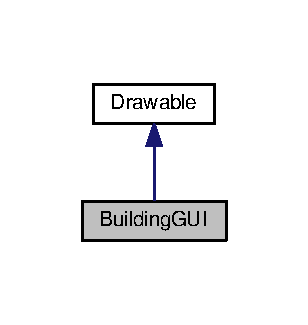
\includegraphics[width=148pt]{classBuildingGUI__inherit__graph}
\end{center}
\end{figure}


Collaboration diagram for Building\-G\-U\-I\-:
\nopagebreak
\begin{figure}[H]
\begin{center}
\leavevmode
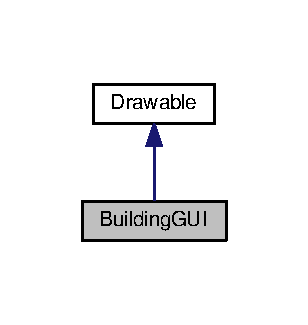
\includegraphics[width=148pt]{classBuildingGUI__coll__graph}
\end{center}
\end{figure}
\subsection*{Public Member Functions}
\begin{DoxyCompactItemize}
\item 
\hyperlink{classBuildingGUI_ad8569800006326c84850f3f34d20a4de}{Building\-G\-U\-I} (Q\-Rect building\-Rect, bool ghost=false)
\begin{DoxyCompactList}\small\item\em \hyperlink{classBuildingGUI_ad8569800006326c84850f3f34d20a4de}{Building\-G\-U\-I\-::\-Building\-G\-U\-I}. Constructor. \end{DoxyCompactList}\item 
\hyperlink{classBuildingGUI_ad98adac46b8a133ecfa03525aeab4475}{Building\-G\-U\-I} (unsigned int x, unsigned int y, unsigned int width=Grid\-G\-U\-I\-::\-S\-I\-Z\-E, unsigned int height=Grid\-G\-U\-I\-::\-S\-I\-Z\-E, bool ghost=false)
\begin{DoxyCompactList}\small\item\em \hyperlink{classBuildingGUI_ad8569800006326c84850f3f34d20a4de}{Building\-G\-U\-I\-::\-Building\-G\-U\-I}. Constructor. \end{DoxyCompactList}\item 
void \hyperlink{classBuildingGUI_ad56a1e74ed82e39bf51743f4d188a302}{draw} (Q\-Painter \&painter) const override
\begin{DoxyCompactList}\small\item\em \hyperlink{classBuildingGUI_ad56a1e74ed82e39bf51743f4d188a302}{Building\-G\-U\-I\-::draw}. \end{DoxyCompactList}\item 
void \hyperlink{classBuildingGUI_a5e193692876cb989f9d7ad83ab9c2450}{set\-To} (unsigned int x, unsigned int y) override
\begin{DoxyCompactList}\small\item\em \hyperlink{classBuildingGUI_a5e193692876cb989f9d7ad83ab9c2450}{Building\-G\-U\-I\-::set\-To}. \end{DoxyCompactList}\item 
bool \hyperlink{classBuildingGUI_a3e6895207c3ca7dc2a61446ddd246de1}{intersects} (Q\-Rect \&rectangle) const override
\begin{DoxyCompactList}\small\item\em \hyperlink{classBuildingGUI_a3e6895207c3ca7dc2a61446ddd246de1}{Building\-G\-U\-I\-::intersects}. \end{DoxyCompactList}\end{DoxyCompactItemize}
\subsection*{Static Public Attributes}
\begin{DoxyCompactItemize}
\item 
static const int \hyperlink{classBuildingGUI_a586063fa325a479fb3f0e6bafb15b052}{P\-E\-N\-\_\-\-W\-I\-D\-T\-H} = 2
\item 
\hypertarget{classBuildingGUI_aff4481c968fbd6718acd5ebd5540ab9e}{static const Qt\-::\-Pen\-Style {\bfseries P\-E\-N\-\_\-\-S\-T\-Y\-L\-E} = Qt\-::\-Solid\-Line}\label{classBuildingGUI_aff4481c968fbd6718acd5ebd5540ab9e}

\item 
\hypertarget{classBuildingGUI_ada34a1c3117d090456d66954730262f5}{static const Qt\-::\-Pen\-Cap\-Style {\bfseries P\-E\-N\-\_\-\-C\-A\-P} = Qt\-::\-Round\-Cap}\label{classBuildingGUI_ada34a1c3117d090456d66954730262f5}

\item 
\hypertarget{classBuildingGUI_a28011806cf0c43237f993b01f6f68ef0}{static const Qt\-::\-Pen\-Join\-Style {\bfseries P\-E\-N\-\_\-\-J\-O\-I\-N} = Qt\-::\-Round\-Join}\label{classBuildingGUI_a28011806cf0c43237f993b01f6f68ef0}

\item 
\hypertarget{classBuildingGUI_a75148840cfcec3abe78d5938f6730549}{static const Q\-Color {\bfseries P\-E\-N\-\_\-\-C\-O\-L\-O\-R} = Q\-Color(0, 0, 0, 255)}\label{classBuildingGUI_a75148840cfcec3abe78d5938f6730549}

\item 
\hypertarget{classBuildingGUI_a179846d692640f271a28cceddf185c4f}{static const Q\-Color {\bfseries G\-H\-O\-S\-T\-\_\-\-P\-E\-N\-\_\-\-C\-O\-L\-O\-R} = Q\-Color(0, 0, 0, 127)}\label{classBuildingGUI_a179846d692640f271a28cceddf185c4f}

\item 
\hypertarget{classBuildingGUI_a2bdc5204e87df75948f8f5c851505218}{static const Q\-Pen {\bfseries P\-E\-N}}\label{classBuildingGUI_a2bdc5204e87df75948f8f5c851505218}

\item 
\hypertarget{classBuildingGUI_afdf9bae63f17079d3ec49d85ff24b0b3}{static const Q\-Pen {\bfseries G\-H\-O\-S\-T\-\_\-\-P\-E\-N}}\label{classBuildingGUI_afdf9bae63f17079d3ec49d85ff24b0b3}

\item 
\hypertarget{classBuildingGUI_ae0eaee99389f670baf7ff080dd2ba774}{static const Qt\-::\-Brush\-Style {\bfseries B\-R\-U\-S\-H\-\_\-\-S\-T\-Y\-L\-E} = Qt\-::\-Solid\-Pattern}\label{classBuildingGUI_ae0eaee99389f670baf7ff080dd2ba774}

\item 
\hypertarget{classBuildingGUI_a2301666ddf31b86c4b47888655ab7e2f}{static const Q\-Color {\bfseries B\-R\-U\-S\-H\-\_\-\-C\-O\-L\-O\-R} = Q\-Color(255, 179, 71)}\label{classBuildingGUI_a2301666ddf31b86c4b47888655ab7e2f}

\item 
\hypertarget{classBuildingGUI_a50a7a863854a4cdf4acb5e2f81f9e427}{static const Q\-Color {\bfseries G\-H\-O\-S\-T\-\_\-\-B\-R\-U\-S\-H\-\_\-\-C\-O\-L\-O\-R} = Q\-Color(255, 179, 71, 127)}\label{classBuildingGUI_a50a7a863854a4cdf4acb5e2f81f9e427}

\item 
\hypertarget{classBuildingGUI_a687bf043be3f6c86fcaf8e927ef8c97f}{static const Q\-Brush {\bfseries B\-R\-U\-S\-H}}\label{classBuildingGUI_a687bf043be3f6c86fcaf8e927ef8c97f}

\item 
\hypertarget{classBuildingGUI_ad92363d651b95a2fed09ba882651581a}{static const Q\-Brush {\bfseries G\-H\-O\-S\-T\-\_\-\-B\-R\-U\-S\-H}}\label{classBuildingGUI_ad92363d651b95a2fed09ba882651581a}

\end{DoxyCompactItemize}


\subsection{Detailed Description}
The \hyperlink{classBuildingGUI}{Building\-G\-U\-I} class. Class holds info about look of building in G\-U\-I. 

Class holds information necessary to draw building in G\-U\-I. It implements virtual functions from base class, so it will be drawn properly. It also impements function for moving object and checking if it intersects with other object. Apart from that it contains all varialbes that decides about look of building in G\-U\-I. \begin{DoxyAuthor}{Author}
Pawel Rybak 
\end{DoxyAuthor}


\subsection{Constructor \& Destructor Documentation}
\hypertarget{classBuildingGUI_ad8569800006326c84850f3f34d20a4de}{\index{Building\-G\-U\-I@{Building\-G\-U\-I}!Building\-G\-U\-I@{Building\-G\-U\-I}}
\index{Building\-G\-U\-I@{Building\-G\-U\-I}!BuildingGUI@{Building\-G\-U\-I}}
\subsubsection[{Building\-G\-U\-I}]{\setlength{\rightskip}{0pt plus 5cm}Building\-G\-U\-I\-::\-Building\-G\-U\-I (
\begin{DoxyParamCaption}
\item[{Q\-Rect}]{building\-Rect, }
\item[{bool}]{ghost = {\ttfamily false}}
\end{DoxyParamCaption}
)}}\label{classBuildingGUI_ad8569800006326c84850f3f34d20a4de}


\hyperlink{classBuildingGUI_ad8569800006326c84850f3f34d20a4de}{Building\-G\-U\-I\-::\-Building\-G\-U\-I}. Constructor. 


\begin{DoxyParams}{Parameters}
{\em building\-Rect} & -\/ Q\-Rect object on which building is based. \\
\hline
{\em ghost} & -\/ flag wheter created object is ghost object or not.\\
\hline
\end{DoxyParams}
Creates \hyperlink{classBuildingGUI}{Building\-G\-U\-I} object based on Q\-Rect object. \hypertarget{classBuildingGUI_ad98adac46b8a133ecfa03525aeab4475}{\index{Building\-G\-U\-I@{Building\-G\-U\-I}!Building\-G\-U\-I@{Building\-G\-U\-I}}
\index{Building\-G\-U\-I@{Building\-G\-U\-I}!BuildingGUI@{Building\-G\-U\-I}}
\subsubsection[{Building\-G\-U\-I}]{\setlength{\rightskip}{0pt plus 5cm}Building\-G\-U\-I\-::\-Building\-G\-U\-I (
\begin{DoxyParamCaption}
\item[{unsigned int}]{x, }
\item[{unsigned int}]{y, }
\item[{unsigned int}]{width = {\ttfamily GridGUI\-:\-:SIZE}, }
\item[{unsigned int}]{height = {\ttfamily GridGUI\-:\-:SIZE}, }
\item[{bool}]{ghost = {\ttfamily false}}
\end{DoxyParamCaption}
)}}\label{classBuildingGUI_ad98adac46b8a133ecfa03525aeab4475}


\hyperlink{classBuildingGUI_ad8569800006326c84850f3f34d20a4de}{Building\-G\-U\-I\-::\-Building\-G\-U\-I}. Constructor. 


\begin{DoxyParams}{Parameters}
{\em x} & -\/ position X of center of top left grid of building. \\
\hline
{\em y} & -\/ position Y of center of top left grid of building. \\
\hline
{\em width} & -\/ building's width. \\
\hline
{\em height} & -\/ building's height. \\
\hline
{\em ghost} & -\/ flag whether object is ghost object.\\
\hline
\end{DoxyParams}
Creates building based on X, Y position and width and height parameters. \hyperlink{classBuilding}{Building}'s top left corner is moved from the X, Y position by half of grid size towartds top left. 

\subsection{Member Function Documentation}
\hypertarget{classBuildingGUI_ad56a1e74ed82e39bf51743f4d188a302}{\index{Building\-G\-U\-I@{Building\-G\-U\-I}!draw@{draw}}
\index{draw@{draw}!BuildingGUI@{Building\-G\-U\-I}}
\subsubsection[{draw}]{\setlength{\rightskip}{0pt plus 5cm}void Building\-G\-U\-I\-::draw (
\begin{DoxyParamCaption}
\item[{Q\-Painter \&}]{painter}
\end{DoxyParamCaption}
) const\hspace{0.3cm}{\ttfamily [override]}, {\ttfamily [virtual]}}}\label{classBuildingGUI_ad56a1e74ed82e39bf51743f4d188a302}


\hyperlink{classBuildingGUI_ad56a1e74ed82e39bf51743f4d188a302}{Building\-G\-U\-I\-::draw}. 


\begin{DoxyParams}{Parameters}
{\em painter} & -\/ Reference to painter object.\\
\hline
\end{DoxyParams}
Function draws object using painter given as an argument. It uses brushes, and pens defined in object, and base its choice on whether it is ghost object or not. 

Implements \hyperlink{classDrawable}{Drawable}.

\hypertarget{classBuildingGUI_a3e6895207c3ca7dc2a61446ddd246de1}{\index{Building\-G\-U\-I@{Building\-G\-U\-I}!intersects@{intersects}}
\index{intersects@{intersects}!BuildingGUI@{Building\-G\-U\-I}}
\subsubsection[{intersects}]{\setlength{\rightskip}{0pt plus 5cm}bool Building\-G\-U\-I\-::intersects (
\begin{DoxyParamCaption}
\item[{Q\-Rect \&}]{rectangle}
\end{DoxyParamCaption}
) const\hspace{0.3cm}{\ttfamily [override]}, {\ttfamily [virtual]}}}\label{classBuildingGUI_a3e6895207c3ca7dc2a61446ddd246de1}


\hyperlink{classBuildingGUI_a3e6895207c3ca7dc2a61446ddd246de1}{Building\-G\-U\-I\-::intersects}. 


\begin{DoxyParams}{Parameters}
{\em rectangle} & -\/ Q\-Rect object that is being checked for intersection. \\
\hline
\end{DoxyParams}
\begin{DoxyReturn}{Returns}
Bool value whether rectangles intersects.
\end{DoxyReturn}
Function checks whether current building's rectangle and rectangle given as argument intersects and returns bool value. 

Implements \hyperlink{classDrawable}{Drawable}.

\hypertarget{classBuildingGUI_a5e193692876cb989f9d7ad83ab9c2450}{\index{Building\-G\-U\-I@{Building\-G\-U\-I}!set\-To@{set\-To}}
\index{set\-To@{set\-To}!BuildingGUI@{Building\-G\-U\-I}}
\subsubsection[{set\-To}]{\setlength{\rightskip}{0pt plus 5cm}void Building\-G\-U\-I\-::set\-To (
\begin{DoxyParamCaption}
\item[{unsigned int}]{x, }
\item[{unsigned int}]{y}
\end{DoxyParamCaption}
)\hspace{0.3cm}{\ttfamily [override]}, {\ttfamily [virtual]}}}\label{classBuildingGUI_a5e193692876cb989f9d7ad83ab9c2450}


\hyperlink{classBuildingGUI_a5e193692876cb989f9d7ad83ab9c2450}{Building\-G\-U\-I\-::set\-To}. 


\begin{DoxyParams}{Parameters}
{\em x} & -\/ position X of center of top left grid of building. \\
\hline
{\em y} & -\/ position Y of center of top left grid of building.\\
\hline
\end{DoxyParams}
Function moves object to point given as arguments. 

Implements \hyperlink{classDrawable}{Drawable}.



\subsection{Member Data Documentation}
\hypertarget{classBuildingGUI_a586063fa325a479fb3f0e6bafb15b052}{\index{Building\-G\-U\-I@{Building\-G\-U\-I}!P\-E\-N\-\_\-\-W\-I\-D\-T\-H@{P\-E\-N\-\_\-\-W\-I\-D\-T\-H}}
\index{P\-E\-N\-\_\-\-W\-I\-D\-T\-H@{P\-E\-N\-\_\-\-W\-I\-D\-T\-H}!BuildingGUI@{Building\-G\-U\-I}}
\subsubsection[{P\-E\-N\-\_\-\-W\-I\-D\-T\-H}]{\setlength{\rightskip}{0pt plus 5cm}const int Building\-G\-U\-I\-::\-P\-E\-N\-\_\-\-W\-I\-D\-T\-H = 2\hspace{0.3cm}{\ttfamily [static]}}}\label{classBuildingGUI_a586063fa325a479fb3f0e6bafb15b052}
P\-R\-O\-P\-E\-R\-T\-I\-E\-S

P\-R\-O\-P\-E\-R\-T\-I\-E\-S I\-N\-I\-T\-I\-A\-L\-I\-Z\-E 

The documentation for this class was generated from the following files\-:\begin{DoxyCompactItemize}
\item 
/home/aleksander/\-C\-Lion\-Projects/\-Zpr/src/\-G\-U\-I/buildinggui.\-h\item 
/home/aleksander/\-C\-Lion\-Projects/\-Zpr/src/\-G\-U\-I/buildinggui.\-cpp\end{DoxyCompactItemize}

\hypertarget{classCamera}{\section{Camera Class Reference}
\label{classCamera}\index{Camera@{Camera}}
}


{\ttfamily \#include $<$Camera.\-h$>$}

\subsection*{Public Member Functions}
\begin{DoxyCompactItemize}
\item 
\hyperlink{classCamera_abe130756ff92b7d9a49eac7a7cbcdbf0}{Camera} (const \hyperlink{classPoint}{Point} \&start\-Point, const \hyperlink{classPoint}{Point} \&end\-Point, double angle, int accuracy)
\item 
bool \hyperlink{classCamera_aca2c02d0712f8e4348ccf1cabac7d582}{is\-In\-Range} (const \hyperlink{classPoint}{Point} \&point)
\item 
bool \hyperlink{classCamera_a8a061df42fe0c6307fbc82e49d85fdff}{is\-In\-Angle} (const \hyperlink{classPoint}{Point} \&point)
\item 
void \hyperlink{classCamera_ac1ec1097de9c1e28283e25b4ca65a2ad}{add\-Seen\-Car} (Ptr\-Const\-Car car)
\item 
\hypertarget{classCamera_a45075ec37bddba6d49c1b38b048ca0ef}{const std\-::vector\\*
$<$ Ptr\-To\-Const\-Point $>$ \& {\bfseries get\-Seen\-Cars} () const }\label{classCamera_a45075ec37bddba6d49c1b38b048ca0ef}

\item 
void \hyperlink{classCamera_a64ea66b871f4dc6408e759f26a4c5267}{add\-Seen\-Human} (Ptr\-Const\-Human human)
\item 
\hypertarget{classCamera_afb7072d894f391afc99595d3590e390d}{const std\-::vector\\*
$<$ Ptr\-To\-Const\-Point $>$ \& {\bfseries get\-Seen\-Humans} () const }\label{classCamera_afb7072d894f391afc99595d3590e390d}

\item 
\hypertarget{classCamera_a174cb7954685f7230bedc91b45d3abc6}{const \hyperlink{classPoint}{Point} \& {\bfseries get\-Start\-Point} () const }\label{classCamera_a174cb7954685f7230bedc91b45d3abc6}

\item 
void \hyperlink{classCamera_ad42a7ec70d41ae24b3ee9d3cd5fad837}{clear\-Seen\-Movables} ()
\end{DoxyCompactItemize}


\subsection{Detailed Description}
This class represents \hyperlink{classCamera}{Camera} as point, angle and ray. \hyperlink{classCamera}{Camera} stores seen cars and humans. \begin{DoxyAuthor}{Author}
Aleksander Brzozowski 
\end{DoxyAuthor}


\subsection{Constructor \& Destructor Documentation}
\hypertarget{classCamera_abe130756ff92b7d9a49eac7a7cbcdbf0}{\index{Camera@{Camera}!Camera@{Camera}}
\index{Camera@{Camera}!Camera@{Camera}}
\subsubsection[{Camera}]{\setlength{\rightskip}{0pt plus 5cm}Camera\-::\-Camera (
\begin{DoxyParamCaption}
\item[{const {\bf Point} \&}]{start\-Point, }
\item[{const {\bf Point} \&}]{end\-Point, }
\item[{double}]{angle, }
\item[{int}]{accuracy}
\end{DoxyParamCaption}
)}}\label{classCamera_abe130756ff92b7d9a49eac7a7cbcdbf0}
Constructs camera. 
\begin{DoxyParams}{Parameters}
{\em start\-Point} & \hyperlink{classPoint}{Point} where camera stands \\
\hline
{\em end\-Point} & \\
\hline
{\em angle} & Visible angle \\
\hline
{\em accuracy} & \hyperlink{classCamera}{Camera}'s accuracy, higher accuracy generates preciser visible points \\
\hline
\end{DoxyParams}


\subsection{Member Function Documentation}
\hypertarget{classCamera_ac1ec1097de9c1e28283e25b4ca65a2ad}{\index{Camera@{Camera}!add\-Seen\-Car@{add\-Seen\-Car}}
\index{add\-Seen\-Car@{add\-Seen\-Car}!Camera@{Camera}}
\subsubsection[{add\-Seen\-Car}]{\setlength{\rightskip}{0pt plus 5cm}void Camera\-::add\-Seen\-Car (
\begin{DoxyParamCaption}
\item[{Ptr\-Const\-Car}]{car}
\end{DoxyParamCaption}
)}}\label{classCamera_ac1ec1097de9c1e28283e25b4ca65a2ad}
Adds car to camera's seen cars. 
\begin{DoxyParams}{Parameters}
{\em car} & \hyperlink{classCar}{Car} to be added \\
\hline
\end{DoxyParams}
\hypertarget{classCamera_a64ea66b871f4dc6408e759f26a4c5267}{\index{Camera@{Camera}!add\-Seen\-Human@{add\-Seen\-Human}}
\index{add\-Seen\-Human@{add\-Seen\-Human}!Camera@{Camera}}
\subsubsection[{add\-Seen\-Human}]{\setlength{\rightskip}{0pt plus 5cm}void Camera\-::add\-Seen\-Human (
\begin{DoxyParamCaption}
\item[{Ptr\-Const\-Human}]{human}
\end{DoxyParamCaption}
)}}\label{classCamera_a64ea66b871f4dc6408e759f26a4c5267}
Adds human to camera's seen humans. 
\begin{DoxyParams}{Parameters}
{\em human} & \hyperlink{classHuman}{Human} to be added \\
\hline
\end{DoxyParams}
\hypertarget{classCamera_ad42a7ec70d41ae24b3ee9d3cd5fad837}{\index{Camera@{Camera}!clear\-Seen\-Movables@{clear\-Seen\-Movables}}
\index{clear\-Seen\-Movables@{clear\-Seen\-Movables}!Camera@{Camera}}
\subsubsection[{clear\-Seen\-Movables}]{\setlength{\rightskip}{0pt plus 5cm}void Camera\-::clear\-Seen\-Movables (
\begin{DoxyParamCaption}
{}
\end{DoxyParamCaption}
)}}\label{classCamera_ad42a7ec70d41ae24b3ee9d3cd5fad837}
Clears all seen cars and humans by camera. \hypertarget{classCamera_a8a061df42fe0c6307fbc82e49d85fdff}{\index{Camera@{Camera}!is\-In\-Angle@{is\-In\-Angle}}
\index{is\-In\-Angle@{is\-In\-Angle}!Camera@{Camera}}
\subsubsection[{is\-In\-Angle}]{\setlength{\rightskip}{0pt plus 5cm}bool Camera\-::is\-In\-Angle (
\begin{DoxyParamCaption}
\item[{const {\bf Point} \&}]{point}
\end{DoxyParamCaption}
)}}\label{classCamera_a8a061df42fe0c6307fbc82e49d85fdff}
Checks whether a point is in camera's angle. 
\begin{DoxyParams}{Parameters}
{\em point} & Checked point \\
\hline
\end{DoxyParams}
\begin{DoxyReturn}{Returns}
Is in camera angle 
\end{DoxyReturn}
\hypertarget{classCamera_aca2c02d0712f8e4348ccf1cabac7d582}{\index{Camera@{Camera}!is\-In\-Range@{is\-In\-Range}}
\index{is\-In\-Range@{is\-In\-Range}!Camera@{Camera}}
\subsubsection[{is\-In\-Range}]{\setlength{\rightskip}{0pt plus 5cm}bool Camera\-::is\-In\-Range (
\begin{DoxyParamCaption}
\item[{const {\bf Point} \&}]{point}
\end{DoxyParamCaption}
)}}\label{classCamera_aca2c02d0712f8e4348ccf1cabac7d582}
Checks whether a point is in camera's range. 
\begin{DoxyParams}{Parameters}
{\em point} & Checked point \\
\hline
\end{DoxyParams}
\begin{DoxyReturn}{Returns}
Is in camera range 
\end{DoxyReturn}


The documentation for this class was generated from the following files\-:\begin{DoxyCompactItemize}
\item 
/home/aleksander/\-C\-Lion\-Projects/\-Zpr/src/Camera.\-h\item 
/home/aleksander/\-C\-Lion\-Projects/\-Zpr/src/Camera.\-cpp\end{DoxyCompactItemize}

\hypertarget{classCameraGUI}{\section{Camera\-G\-U\-I Class Reference}
\label{classCameraGUI}\index{Camera\-G\-U\-I@{Camera\-G\-U\-I}}
}


The \hyperlink{classCameraGUI}{Camera\-G\-U\-I} class. Class holds info about look of camera in G\-U\-I.  




{\ttfamily \#include $<$cameragui.\-h$>$}



Inheritance diagram for Camera\-G\-U\-I\-:
\nopagebreak
\begin{figure}[H]
\begin{center}
\leavevmode
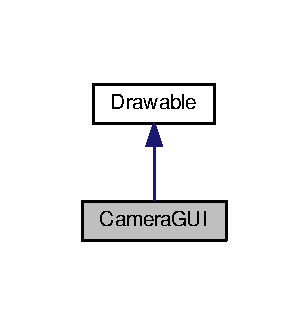
\includegraphics[width=148pt]{classCameraGUI__inherit__graph}
\end{center}
\end{figure}


Collaboration diagram for Camera\-G\-U\-I\-:
\nopagebreak
\begin{figure}[H]
\begin{center}
\leavevmode
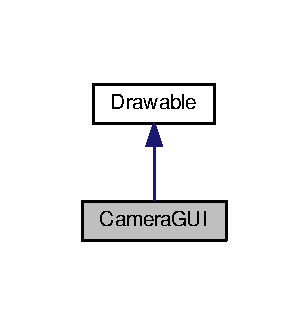
\includegraphics[width=148pt]{classCameraGUI__coll__graph}
\end{center}
\end{figure}
\subsection*{Public Member Functions}
\begin{DoxyCompactItemize}
\item 
\hyperlink{classCameraGUI_a076ea3f14aace383a31d4cd835310a49}{Camera\-G\-U\-I} (unsigned int x, unsigned int y, unsigned int span, int angle, unsigned int range, bool ghost=false)
\begin{DoxyCompactList}\small\item\em \hyperlink{classCameraGUI_a076ea3f14aace383a31d4cd835310a49}{Camera\-G\-U\-I\-::\-Camera\-G\-U\-I}. Constructor. \end{DoxyCompactList}\item 
\hyperlink{classCameraGUI_a847265abc60ee2011e460e20f8e17930}{Camera\-G\-U\-I} (\hyperlink{classPoint}{Point} position, \hyperlink{classPoint}{Point} range, int span, bool ghost=false)
\begin{DoxyCompactList}\small\item\em \hyperlink{classCameraGUI_a076ea3f14aace383a31d4cd835310a49}{Camera\-G\-U\-I\-::\-Camera\-G\-U\-I}. Constructor. \end{DoxyCompactList}\item 
\hyperlink{classCameraGUI_aee52d51f94af00b5f70673d36bb7f8df}{Camera\-G\-U\-I} (\hyperlink{classPoint}{Point} position)
\begin{DoxyCompactList}\small\item\em \hyperlink{classCameraGUI_a076ea3f14aace383a31d4cd835310a49}{Camera\-G\-U\-I\-::\-Camera\-G\-U\-I}. Constructor. \end{DoxyCompactList}\item 
void \hyperlink{classCameraGUI_ac2f1343cecf2469c4112bc3efe122b1f}{set\-Rectangle} (\hyperlink{classPoint}{Point} point)
\begin{DoxyCompactList}\small\item\em \hyperlink{classCameraGUI_ac2f1343cecf2469c4112bc3efe122b1f}{Camera\-G\-U\-I\-::set\-Rectangle}. \end{DoxyCompactList}\item 
void \hyperlink{classCameraGUI_a9c7dedccd547b24aeea2275b81964dd5}{set\-Rectangle} (\hyperlink{classPoint}{Point} first, \hyperlink{classPoint}{Point} second)
\begin{DoxyCompactList}\small\item\em \hyperlink{classCameraGUI_ac2f1343cecf2469c4112bc3efe122b1f}{Camera\-G\-U\-I\-::set\-Rectangle}. \end{DoxyCompactList}\item 
void \hyperlink{classCameraGUI_a56c36908fcf541131711a96be0d19bf2}{draw} (Q\-Painter \&) const 
\begin{DoxyCompactList}\small\item\em \hyperlink{classCameraGUI_a56c36908fcf541131711a96be0d19bf2}{Camera\-G\-U\-I\-::draw}. \end{DoxyCompactList}\item 
\hypertarget{classCameraGUI_a70a05a7d985c73ddc47f4967c4b7de19}{void {\bfseries set\-To} (unsigned int x, unsigned int y) override}\label{classCameraGUI_a70a05a7d985c73ddc47f4967c4b7de19}

\item 
bool \hyperlink{classCameraGUI_a9a7be75113cbe6618df95d29a7184ae9}{intersects} (Q\-Rect \&rectangle) const 
\begin{DoxyCompactList}\small\item\em \hyperlink{classCameraGUI_a9a7be75113cbe6618df95d29a7184ae9}{Camera\-G\-U\-I\-::intersects}. \end{DoxyCompactList}\item 
void \hyperlink{classCameraGUI_a899d0ba69e44e61bd8f993e70dd8bf58}{dec\-Range} ()
\begin{DoxyCompactList}\small\item\em \hyperlink{classCameraGUI_a899d0ba69e44e61bd8f993e70dd8bf58}{Camera\-G\-U\-I\-::dec\-Range}. \end{DoxyCompactList}\item 
void \hyperlink{classCameraGUI_ae5a54018d6985ac4fae5f69e49e54a80}{inc\-Range} ()
\begin{DoxyCompactList}\small\item\em \hyperlink{classCameraGUI_ae5a54018d6985ac4fae5f69e49e54a80}{Camera\-G\-U\-I\-::inc\-Range}. \end{DoxyCompactList}\item 
void \hyperlink{classCameraGUI_a9bd87784914772edd3fea9d12b5119c7}{rot\-Clockwise} ()
\begin{DoxyCompactList}\small\item\em \hyperlink{classCameraGUI_a9bd87784914772edd3fea9d12b5119c7}{Camera\-G\-U\-I\-::rot\-Clockwise}. \end{DoxyCompactList}\item 
void \hyperlink{classCameraGUI_a0ba57c92828cd8ee6aa4b1af2b42e4a7}{rot\-Counterclockwise} ()
\begin{DoxyCompactList}\small\item\em \hyperlink{classCameraGUI_a0ba57c92828cd8ee6aa4b1af2b42e4a7}{Camera\-G\-U\-I\-::rot\-Counterclockwise}. \end{DoxyCompactList}\item 
void \hyperlink{classCameraGUI_a525f57d02a5324bb4e55bfa13001bd9e}{inc\-Span} ()
\begin{DoxyCompactList}\small\item\em \hyperlink{classCameraGUI_a525f57d02a5324bb4e55bfa13001bd9e}{Camera\-G\-U\-I\-::inc\-Span}. \end{DoxyCompactList}\item 
void \hyperlink{classCameraGUI_a626ff2fa3927c2292e16187e1ecef422}{dec\-Span} ()
\begin{DoxyCompactList}\small\item\em \hyperlink{classCameraGUI_a626ff2fa3927c2292e16187e1ecef422}{Camera\-G\-U\-I\-::dec\-Span}. \end{DoxyCompactList}\item 
int \hyperlink{classCameraGUI_a6e3b89ea4a94a7ad90ab295556173be5}{get\-Span} ()
\begin{DoxyCompactList}\small\item\em \hyperlink{classCameraGUI_a6e3b89ea4a94a7ad90ab295556173be5}{Camera\-G\-U\-I\-::get\-Span}. \end{DoxyCompactList}\item 
int \hyperlink{classCameraGUI_a948fc684449338f3f0d4c4e02692234b}{get\-Angle} ()
\begin{DoxyCompactList}\small\item\em \hyperlink{classCameraGUI_a948fc684449338f3f0d4c4e02692234b}{Camera\-G\-U\-I\-::get\-Angle}. \end{DoxyCompactList}\item 
int \hyperlink{classCameraGUI_a3da1bc7c4ab1c7d56f918dd21873a862}{get\-Range} ()
\begin{DoxyCompactList}\small\item\em \hyperlink{classCameraGUI_a3da1bc7c4ab1c7d56f918dd21873a862}{Camera\-G\-U\-I\-::get\-Range}. \end{DoxyCompactList}\end{DoxyCompactItemize}
\subsection*{Static Public Attributes}
\begin{DoxyCompactItemize}
\item 
static const unsigned int \hyperlink{classCameraGUI_a3bfd5efeeb6e8474ff4d1106440ca1ab}{C\-A\-M\-\_\-\-R\-A\-D\-I\-U\-S} = 8
\item 
\hypertarget{classCameraGUI_a7f8ecb7208f8d6256f5eeb18db936244}{static const unsigned int {\bfseries M\-A\-X\-\_\-\-R\-A\-N\-G\-E} = 5 $\ast$ Grid\-G\-U\-I\-::\-S\-I\-Z\-E}\label{classCameraGUI_a7f8ecb7208f8d6256f5eeb18db936244}

\item 
\hypertarget{classCameraGUI_adc4a994ad297cfff1e76c1e00bced733}{static const unsigned int {\bfseries M\-I\-N\-\_\-\-R\-A\-N\-G\-E} = 100}\label{classCameraGUI_adc4a994ad297cfff1e76c1e00bced733}

\item 
\hypertarget{classCameraGUI_a0bab41ff4cf14b5b7e3256a780792fd1}{static const unsigned int {\bfseries M\-A\-X\-\_\-\-S\-P\-A\-N} = 180}\label{classCameraGUI_a0bab41ff4cf14b5b7e3256a780792fd1}

\item 
\hypertarget{classCameraGUI_ab92e05091879d7af4c710be042bea717}{static const unsigned int {\bfseries M\-I\-N\-\_\-\-S\-P\-A\-N} = 10}\label{classCameraGUI_ab92e05091879d7af4c710be042bea717}

\item 
\hypertarget{classCameraGUI_a4757b83877c8a4dcc70d1025df24fb9f}{static const int {\bfseries D\-E\-F\-A\-U\-L\-T\-\_\-\-S\-P\-A\-N} = 60}\label{classCameraGUI_a4757b83877c8a4dcc70d1025df24fb9f}

\item 
\hypertarget{classCameraGUI_a9562f728089b5066cb0fd5e09b64dcaa}{static const int {\bfseries D\-E\-F\-A\-U\-L\-T\-\_\-\-A\-N\-G\-L\-E} = -\/D\-E\-F\-A\-U\-L\-T\-\_\-\-S\-P\-A\-N/2}\label{classCameraGUI_a9562f728089b5066cb0fd5e09b64dcaa}

\item 
\hypertarget{classCameraGUI_a1870cb9bfe4d69423954af5153b5e6dc}{static const unsigned int {\bfseries D\-E\-F\-A\-U\-L\-T\-\_\-\-R\-A\-N\-G\-E} = 200}\label{classCameraGUI_a1870cb9bfe4d69423954af5153b5e6dc}

\item 
\hypertarget{classCameraGUI_ad29d1cc52182c76904726d279082a4eb}{static const int {\bfseries C\-A\-M\-\_\-\-P\-E\-N\-\_\-\-W\-I\-D\-T\-H} = 2}\label{classCameraGUI_ad29d1cc52182c76904726d279082a4eb}

\item 
\hypertarget{classCameraGUI_ac202b5df044399e3ccf1c41181f0c390}{static const Qt\-::\-Pen\-Style {\bfseries C\-A\-M\-\_\-\-P\-E\-N\-\_\-\-S\-T\-Y\-L\-E} = Qt\-::\-Solid\-Line}\label{classCameraGUI_ac202b5df044399e3ccf1c41181f0c390}

\item 
\hypertarget{classCameraGUI_a2e99509394c107afdb1de6167a137de2}{static const Qt\-::\-Pen\-Cap\-Style {\bfseries C\-A\-M\-\_\-\-P\-E\-N\-\_\-\-C\-A\-P} = Qt\-::\-Square\-Cap}\label{classCameraGUI_a2e99509394c107afdb1de6167a137de2}

\item 
\hypertarget{classCameraGUI_ab6ebad56d837fb8a910dff37b075127f}{static const Qt\-::\-Pen\-Join\-Style {\bfseries C\-A\-M\-\_\-\-P\-E\-N\-\_\-\-J\-O\-I\-N} = Qt\-::\-Round\-Join}\label{classCameraGUI_ab6ebad56d837fb8a910dff37b075127f}

\item 
\hypertarget{classCameraGUI_adcbeae7987dad32eae5d7532c4057ac1}{static const Q\-Color {\bfseries C\-A\-M\-\_\-\-P\-E\-N\-\_\-\-C\-O\-L\-O\-R} = Q\-Color(0, 0, 0)}\label{classCameraGUI_adcbeae7987dad32eae5d7532c4057ac1}

\item 
\hypertarget{classCameraGUI_a0d3c759a8f5c7e781bbb307b1cc2adf6}{static const Q\-Color {\bfseries G\-H\-O\-S\-T\-\_\-\-C\-A\-M\-\_\-\-P\-E\-N\-\_\-\-C\-O\-L\-O\-R} = Q\-Color(0, 0, 0, 127)}\label{classCameraGUI_a0d3c759a8f5c7e781bbb307b1cc2adf6}

\item 
\hypertarget{classCameraGUI_a298a8aa3eacaf56edeb881be5ad09f96}{static const Q\-Pen {\bfseries C\-A\-M\-\_\-\-P\-E\-N}}\label{classCameraGUI_a298a8aa3eacaf56edeb881be5ad09f96}

\item 
\hypertarget{classCameraGUI_ad6cb3916341cedc82c1c110487a20e8a}{static const Q\-Pen {\bfseries G\-H\-O\-S\-T\-\_\-\-C\-A\-M\-\_\-\-P\-E\-N}}\label{classCameraGUI_ad6cb3916341cedc82c1c110487a20e8a}

\item 
\hypertarget{classCameraGUI_a5dae39bcabadb82d30643023e694df53}{static const Qt\-::\-Brush\-Style {\bfseries C\-A\-M\-\_\-\-B\-R\-U\-S\-H\-\_\-\-S\-T\-Y\-L\-E} = Qt\-::\-Solid\-Pattern}\label{classCameraGUI_a5dae39bcabadb82d30643023e694df53}

\item 
\hypertarget{classCameraGUI_acb2690e862c3a4910494b41d10c71673}{static const Q\-Color {\bfseries C\-A\-M\-\_\-\-B\-R\-U\-S\-H\-\_\-\-C\-O\-L\-O\-R} = Q\-Color(103, 74, 158)}\label{classCameraGUI_acb2690e862c3a4910494b41d10c71673}

\item 
\hypertarget{classCameraGUI_a0fffcb81bdb6e757d8b22eb0fc300d63}{static const Q\-Color {\bfseries G\-H\-O\-S\-T\-\_\-\-C\-A\-M\-\_\-\-B\-R\-U\-S\-H\-\_\-\-C\-O\-L\-O\-R} = Q\-Color(103, 74, 158, 127)}\label{classCameraGUI_a0fffcb81bdb6e757d8b22eb0fc300d63}

\item 
\hypertarget{classCameraGUI_a098d01461f680aff5b47d09235e6748a}{static const Q\-Brush {\bfseries C\-A\-M\-\_\-\-B\-R\-U\-S\-H}}\label{classCameraGUI_a098d01461f680aff5b47d09235e6748a}

\item 
\hypertarget{classCameraGUI_ae939ce3f55739a8b8d9cf9b6740da91d}{static const Q\-Brush {\bfseries G\-H\-O\-S\-T\-\_\-\-C\-A\-M\-\_\-\-B\-R\-U\-S\-H}}\label{classCameraGUI_ae939ce3f55739a8b8d9cf9b6740da91d}

\item 
\hypertarget{classCameraGUI_af5a35c36f4043bd723778f4488009b35}{static const int {\bfseries R\-N\-G\-\_\-\-P\-E\-N\-\_\-\-W\-I\-D\-T\-H} = 0}\label{classCameraGUI_af5a35c36f4043bd723778f4488009b35}

\item 
\hypertarget{classCameraGUI_af9e000abeddf2a871e2d5ef4d08773bf}{static const Qt\-::\-Pen\-Style {\bfseries R\-N\-G\-\_\-\-P\-E\-N\-\_\-\-S\-T\-Y\-L\-E} = Qt\-::\-Solid\-Line}\label{classCameraGUI_af9e000abeddf2a871e2d5ef4d08773bf}

\item 
\hypertarget{classCameraGUI_a042cca0636bb39244a0a689af8f62b17}{static const Qt\-::\-Pen\-Cap\-Style {\bfseries R\-N\-G\-\_\-\-P\-E\-N\-\_\-\-C\-A\-P} = Qt\-::\-Square\-Cap}\label{classCameraGUI_a042cca0636bb39244a0a689af8f62b17}

\item 
\hypertarget{classCameraGUI_a6d4f35cefc63050d44b5a1271059653c}{static const Qt\-::\-Pen\-Join\-Style {\bfseries R\-N\-G\-\_\-\-P\-E\-N\-\_\-\-J\-O\-I\-N} = Qt\-::\-Round\-Join}\label{classCameraGUI_a6d4f35cefc63050d44b5a1271059653c}

\item 
\hypertarget{classCameraGUI_aec90c5accd29fffeb8735551d6f66f23}{static const Q\-Color {\bfseries R\-N\-G\-\_\-\-P\-E\-N\-\_\-\-C\-O\-L\-O\-R} = Q\-Color(0, 0, 0, 0)}\label{classCameraGUI_aec90c5accd29fffeb8735551d6f66f23}

\item 
\hypertarget{classCameraGUI_a4d24939af4bb409df6b89b0cb974074c}{static const Q\-Color {\bfseries G\-H\-O\-S\-T\-\_\-\-R\-N\-G\-\_\-\-P\-E\-N\-\_\-\-C\-O\-L\-O\-R} = Q\-Color(0, 0, 0, 0)}\label{classCameraGUI_a4d24939af4bb409df6b89b0cb974074c}

\item 
\hypertarget{classCameraGUI_a2ad79374ad1db2e7fe7364b262825851}{static const Q\-Pen {\bfseries R\-N\-G\-\_\-\-P\-E\-N}}\label{classCameraGUI_a2ad79374ad1db2e7fe7364b262825851}

\item 
\hypertarget{classCameraGUI_a67439a62df649c6f76b0663dc3d14c09}{static const Q\-Pen {\bfseries G\-H\-O\-S\-T\-\_\-\-R\-N\-G\-\_\-\-P\-E\-N}}\label{classCameraGUI_a67439a62df649c6f76b0663dc3d14c09}

\item 
\hypertarget{classCameraGUI_a01530501f6b9e651ac94000aeb94ea1f}{static const Qt\-::\-Brush\-Style {\bfseries R\-N\-G\-\_\-\-B\-R\-U\-S\-H\-\_\-\-S\-T\-Y\-L\-E} = Qt\-::\-Solid\-Pattern}\label{classCameraGUI_a01530501f6b9e651ac94000aeb94ea1f}

\item 
\hypertarget{classCameraGUI_acc2e2bc371644b94c99d1c9d35688048}{static const Q\-Color {\bfseries R\-N\-G\-\_\-\-B\-R\-U\-S\-H\-\_\-\-C\-O\-L\-O\-R} = Q\-Color(177, 156, 217, 127)}\label{classCameraGUI_acc2e2bc371644b94c99d1c9d35688048}

\item 
\hypertarget{classCameraGUI_a8689b5f981805945dd4c1c251e7065e5}{static const Q\-Color {\bfseries G\-H\-O\-S\-T\-\_\-\-R\-N\-G\-\_\-\-B\-R\-U\-S\-H\-\_\-\-C\-O\-L\-O\-R} = Q\-Color(177, 156, 217, 64)}\label{classCameraGUI_a8689b5f981805945dd4c1c251e7065e5}

\item 
\hypertarget{classCameraGUI_a1f46ce78c9696e44e1330f591df3f5c4}{static const Q\-Brush {\bfseries R\-N\-G\-\_\-\-B\-R\-U\-S\-H}}\label{classCameraGUI_a1f46ce78c9696e44e1330f591df3f5c4}

\item 
\hypertarget{classCameraGUI_a3fd5e88f6a785f92bec36a9bb783eee9}{static const Q\-Brush {\bfseries G\-H\-O\-S\-T\-\_\-\-R\-N\-G\-\_\-\-B\-R\-U\-S\-H}}\label{classCameraGUI_a3fd5e88f6a785f92bec36a9bb783eee9}

\end{DoxyCompactItemize}


\subsection{Detailed Description}
The \hyperlink{classCameraGUI}{Camera\-G\-U\-I} class. Class holds info about look of camera in G\-U\-I. 

Class holds information necessary to draw camera in G\-U\-I. It implements virtual function from base class, so it wil be drawn poperly. It has also function that allows io move it and differ its range of sight. Function holds all information about the look of the camera on screen. \begin{DoxyAuthor}{Author}
Pawel Rybak 
\end{DoxyAuthor}


\subsection{Constructor \& Destructor Documentation}
\hypertarget{classCameraGUI_a076ea3f14aace383a31d4cd835310a49}{\index{Camera\-G\-U\-I@{Camera\-G\-U\-I}!Camera\-G\-U\-I@{Camera\-G\-U\-I}}
\index{Camera\-G\-U\-I@{Camera\-G\-U\-I}!CameraGUI@{Camera\-G\-U\-I}}
\subsubsection[{Camera\-G\-U\-I}]{\setlength{\rightskip}{0pt plus 5cm}Camera\-G\-U\-I\-::\-Camera\-G\-U\-I (
\begin{DoxyParamCaption}
\item[{unsigned int}]{x, }
\item[{unsigned int}]{y, }
\item[{unsigned int}]{span, }
\item[{int}]{angle, }
\item[{unsigned int}]{range, }
\item[{bool}]{ghost = {\ttfamily false}}
\end{DoxyParamCaption}
)}}\label{classCameraGUI_a076ea3f14aace383a31d4cd835310a49}


\hyperlink{classCameraGUI_a076ea3f14aace383a31d4cd835310a49}{Camera\-G\-U\-I\-::\-Camera\-G\-U\-I}. Constructor. 


\begin{DoxyParams}{Parameters}
{\em x} & -\/ Position X of camera. \\
\hline
{\em y} & -\/ Position Y of camera. \\
\hline
{\em span} & -\/ camera's sight span. Unit is 1/16th of a degree. \\
\hline
{\em angle} & -\/ Direction of camera's sigh. Angle 0 is bottom of sight starts paralell to x axis to the left. Increasing turns it counterclockwise. Unit is 1/16th of a degree. \\
\hline
{\em range} & -\/ \hyperlink{classCamera}{Camera}'s range of view. \\
\hline
{\em ghost} & -\/ Boolean tells whether object is ghost object or not.\\
\hline
\end{DoxyParams}
Constructor creates camera object centered at point X, Y given as parameters. \hypertarget{classCameraGUI_a847265abc60ee2011e460e20f8e17930}{\index{Camera\-G\-U\-I@{Camera\-G\-U\-I}!Camera\-G\-U\-I@{Camera\-G\-U\-I}}
\index{Camera\-G\-U\-I@{Camera\-G\-U\-I}!CameraGUI@{Camera\-G\-U\-I}}
\subsubsection[{Camera\-G\-U\-I}]{\setlength{\rightskip}{0pt plus 5cm}Camera\-G\-U\-I\-::\-Camera\-G\-U\-I (
\begin{DoxyParamCaption}
\item[{{\bf Point}}]{position, }
\item[{{\bf Point}}]{range, }
\item[{int}]{span, }
\item[{bool}]{ghost = {\ttfamily false}}
\end{DoxyParamCaption}
)}}\label{classCameraGUI_a847265abc60ee2011e460e20f8e17930}


\hyperlink{classCameraGUI_a076ea3f14aace383a31d4cd835310a49}{Camera\-G\-U\-I\-::\-Camera\-G\-U\-I}. Constructor. 


\begin{DoxyParams}{Parameters}
{\em position} & -\/ Position of a camera. \\
\hline
{\em range} & -\/ \hyperlink{classPoint}{Point} where camera's range ends. \\
\hline
{\em span} & -\/ cmaera's cpan. Unit is 1/16th of a degree. \\
\hline
{\em ghost} & -\/ Boolean tells whether object is ghost object or not.\\
\hline
\end{DoxyParams}
Constructor creates camera a given point with range ending and another point given as argument. \hypertarget{classCameraGUI_aee52d51f94af00b5f70673d36bb7f8df}{\index{Camera\-G\-U\-I@{Camera\-G\-U\-I}!Camera\-G\-U\-I@{Camera\-G\-U\-I}}
\index{Camera\-G\-U\-I@{Camera\-G\-U\-I}!CameraGUI@{Camera\-G\-U\-I}}
\subsubsection[{Camera\-G\-U\-I}]{\setlength{\rightskip}{0pt plus 5cm}Camera\-G\-U\-I\-::\-Camera\-G\-U\-I (
\begin{DoxyParamCaption}
\item[{{\bf Point}}]{position}
\end{DoxyParamCaption}
)}}\label{classCameraGUI_aee52d51f94af00b5f70673d36bb7f8df}


\hyperlink{classCameraGUI_a076ea3f14aace383a31d4cd835310a49}{Camera\-G\-U\-I\-::\-Camera\-G\-U\-I}. Constructor. 


\begin{DoxyParams}{Parameters}
{\em position} & -\/ Position of a camera.\\
\hline
\end{DoxyParams}
Constructor creates camera centered at a position given as parameter. It's range of view is set to zero. Object constructed with that function is always ghost object. 

\subsection{Member Function Documentation}
\hypertarget{classCameraGUI_a899d0ba69e44e61bd8f993e70dd8bf58}{\index{Camera\-G\-U\-I@{Camera\-G\-U\-I}!dec\-Range@{dec\-Range}}
\index{dec\-Range@{dec\-Range}!CameraGUI@{Camera\-G\-U\-I}}
\subsubsection[{dec\-Range}]{\setlength{\rightskip}{0pt plus 5cm}void Camera\-G\-U\-I\-::dec\-Range (
\begin{DoxyParamCaption}
{}
\end{DoxyParamCaption}
)}}\label{classCameraGUI_a899d0ba69e44e61bd8f993e70dd8bf58}


\hyperlink{classCameraGUI_a899d0ba69e44e61bd8f993e70dd8bf58}{Camera\-G\-U\-I\-::dec\-Range}. 

Decrements range by 10 pixels unless it is minimum already. Limits are defined in object. \hypertarget{classCameraGUI_a626ff2fa3927c2292e16187e1ecef422}{\index{Camera\-G\-U\-I@{Camera\-G\-U\-I}!dec\-Span@{dec\-Span}}
\index{dec\-Span@{dec\-Span}!CameraGUI@{Camera\-G\-U\-I}}
\subsubsection[{dec\-Span}]{\setlength{\rightskip}{0pt plus 5cm}void Camera\-G\-U\-I\-::dec\-Span (
\begin{DoxyParamCaption}
{}
\end{DoxyParamCaption}
)}}\label{classCameraGUI_a626ff2fa3927c2292e16187e1ecef422}


\hyperlink{classCameraGUI_a626ff2fa3927c2292e16187e1ecef422}{Camera\-G\-U\-I\-::dec\-Span}. 

Decrements camera's view span by 1 degree unless it is minimum already. Limits are defined in object. \hypertarget{classCameraGUI_a56c36908fcf541131711a96be0d19bf2}{\index{Camera\-G\-U\-I@{Camera\-G\-U\-I}!draw@{draw}}
\index{draw@{draw}!CameraGUI@{Camera\-G\-U\-I}}
\subsubsection[{draw}]{\setlength{\rightskip}{0pt plus 5cm}void Camera\-G\-U\-I\-::draw (
\begin{DoxyParamCaption}
\item[{Q\-Painter \&}]{painter}
\end{DoxyParamCaption}
) const\hspace{0.3cm}{\ttfamily [virtual]}}}\label{classCameraGUI_a56c36908fcf541131711a96be0d19bf2}


\hyperlink{classCameraGUI_a56c36908fcf541131711a96be0d19bf2}{Camera\-G\-U\-I\-::draw}. 


\begin{DoxyParams}{Parameters}
{\em painter} & -\/ Reference to painter object.\\
\hline
\end{DoxyParams}
Function draws object using painter given as an argument. It uses brushes, and pens defined in object, and base its choice on whether it is ghost object or not. 

Implements \hyperlink{classDrawable}{Drawable}.

\hypertarget{classCameraGUI_a948fc684449338f3f0d4c4e02692234b}{\index{Camera\-G\-U\-I@{Camera\-G\-U\-I}!get\-Angle@{get\-Angle}}
\index{get\-Angle@{get\-Angle}!CameraGUI@{Camera\-G\-U\-I}}
\subsubsection[{get\-Angle}]{\setlength{\rightskip}{0pt plus 5cm}int Camera\-G\-U\-I\-::get\-Angle (
\begin{DoxyParamCaption}
{}
\end{DoxyParamCaption}
)}}\label{classCameraGUI_a948fc684449338f3f0d4c4e02692234b}


\hyperlink{classCameraGUI_a948fc684449338f3f0d4c4e02692234b}{Camera\-G\-U\-I\-::get\-Angle}. 

\begin{DoxyReturn}{Returns}
Returns current angle. Unit is 1/16th of degree. 
\end{DoxyReturn}
\hypertarget{classCameraGUI_a3da1bc7c4ab1c7d56f918dd21873a862}{\index{Camera\-G\-U\-I@{Camera\-G\-U\-I}!get\-Range@{get\-Range}}
\index{get\-Range@{get\-Range}!CameraGUI@{Camera\-G\-U\-I}}
\subsubsection[{get\-Range}]{\setlength{\rightskip}{0pt plus 5cm}int Camera\-G\-U\-I\-::get\-Range (
\begin{DoxyParamCaption}
{}
\end{DoxyParamCaption}
)}}\label{classCameraGUI_a3da1bc7c4ab1c7d56f918dd21873a862}


\hyperlink{classCameraGUI_a3da1bc7c4ab1c7d56f918dd21873a862}{Camera\-G\-U\-I\-::get\-Range}. 

\begin{DoxyReturn}{Returns}
Returns current range. Units are pixels. 
\end{DoxyReturn}
\hypertarget{classCameraGUI_a6e3b89ea4a94a7ad90ab295556173be5}{\index{Camera\-G\-U\-I@{Camera\-G\-U\-I}!get\-Span@{get\-Span}}
\index{get\-Span@{get\-Span}!CameraGUI@{Camera\-G\-U\-I}}
\subsubsection[{get\-Span}]{\setlength{\rightskip}{0pt plus 5cm}int Camera\-G\-U\-I\-::get\-Span (
\begin{DoxyParamCaption}
{}
\end{DoxyParamCaption}
)}}\label{classCameraGUI_a6e3b89ea4a94a7ad90ab295556173be5}


\hyperlink{classCameraGUI_a6e3b89ea4a94a7ad90ab295556173be5}{Camera\-G\-U\-I\-::get\-Span}. 

\begin{DoxyReturn}{Returns}
Returns current span. Unit is 1/16th of degree. 
\end{DoxyReturn}
\hypertarget{classCameraGUI_ae5a54018d6985ac4fae5f69e49e54a80}{\index{Camera\-G\-U\-I@{Camera\-G\-U\-I}!inc\-Range@{inc\-Range}}
\index{inc\-Range@{inc\-Range}!CameraGUI@{Camera\-G\-U\-I}}
\subsubsection[{inc\-Range}]{\setlength{\rightskip}{0pt plus 5cm}void Camera\-G\-U\-I\-::inc\-Range (
\begin{DoxyParamCaption}
{}
\end{DoxyParamCaption}
)}}\label{classCameraGUI_ae5a54018d6985ac4fae5f69e49e54a80}


\hyperlink{classCameraGUI_ae5a54018d6985ac4fae5f69e49e54a80}{Camera\-G\-U\-I\-::inc\-Range}. 

Increments range by 10 pixels unless it is maximum already. Limits are defined in object. \hypertarget{classCameraGUI_a525f57d02a5324bb4e55bfa13001bd9e}{\index{Camera\-G\-U\-I@{Camera\-G\-U\-I}!inc\-Span@{inc\-Span}}
\index{inc\-Span@{inc\-Span}!CameraGUI@{Camera\-G\-U\-I}}
\subsubsection[{inc\-Span}]{\setlength{\rightskip}{0pt plus 5cm}void Camera\-G\-U\-I\-::inc\-Span (
\begin{DoxyParamCaption}
{}
\end{DoxyParamCaption}
)}}\label{classCameraGUI_a525f57d02a5324bb4e55bfa13001bd9e}


\hyperlink{classCameraGUI_a525f57d02a5324bb4e55bfa13001bd9e}{Camera\-G\-U\-I\-::inc\-Span}. 

Increments camera's view span by 1 degree unless it is maximum already. Limits are defined in object. \hypertarget{classCameraGUI_a9a7be75113cbe6618df95d29a7184ae9}{\index{Camera\-G\-U\-I@{Camera\-G\-U\-I}!intersects@{intersects}}
\index{intersects@{intersects}!CameraGUI@{Camera\-G\-U\-I}}
\subsubsection[{intersects}]{\setlength{\rightskip}{0pt plus 5cm}bool Camera\-G\-U\-I\-::intersects (
\begin{DoxyParamCaption}
\item[{Q\-Rect \&}]{rectangle}
\end{DoxyParamCaption}
) const\hspace{0.3cm}{\ttfamily [virtual]}}}\label{classCameraGUI_a9a7be75113cbe6618df95d29a7184ae9}


\hyperlink{classCameraGUI_a9a7be75113cbe6618df95d29a7184ae9}{Camera\-G\-U\-I\-::intersects}. 


\begin{DoxyParams}{Parameters}
{\em rectangle} & -\/ Q\-Rect object that is being checked for intersection. \\
\hline
\end{DoxyParams}
\begin{DoxyReturn}{Returns}
Bool value whether rectangles intersects.
\end{DoxyReturn}
Function checks whether current camera's (not including sight range) rectangle intersects rectangle given as argument and returns bool value. 

Implements \hyperlink{classDrawable}{Drawable}.

\hypertarget{classCameraGUI_a9bd87784914772edd3fea9d12b5119c7}{\index{Camera\-G\-U\-I@{Camera\-G\-U\-I}!rot\-Clockwise@{rot\-Clockwise}}
\index{rot\-Clockwise@{rot\-Clockwise}!CameraGUI@{Camera\-G\-U\-I}}
\subsubsection[{rot\-Clockwise}]{\setlength{\rightskip}{0pt plus 5cm}void Camera\-G\-U\-I\-::rot\-Clockwise (
\begin{DoxyParamCaption}
{}
\end{DoxyParamCaption}
)}}\label{classCameraGUI_a9bd87784914772edd3fea9d12b5119c7}


\hyperlink{classCameraGUI_a9bd87784914772edd3fea9d12b5119c7}{Camera\-G\-U\-I\-::rot\-Clockwise}. 

Rotates camera's view by 1 degree clockwise. \hypertarget{classCameraGUI_a0ba57c92828cd8ee6aa4b1af2b42e4a7}{\index{Camera\-G\-U\-I@{Camera\-G\-U\-I}!rot\-Counterclockwise@{rot\-Counterclockwise}}
\index{rot\-Counterclockwise@{rot\-Counterclockwise}!CameraGUI@{Camera\-G\-U\-I}}
\subsubsection[{rot\-Counterclockwise}]{\setlength{\rightskip}{0pt plus 5cm}void Camera\-G\-U\-I\-::rot\-Counterclockwise (
\begin{DoxyParamCaption}
{}
\end{DoxyParamCaption}
)}}\label{classCameraGUI_a0ba57c92828cd8ee6aa4b1af2b42e4a7}


\hyperlink{classCameraGUI_a0ba57c92828cd8ee6aa4b1af2b42e4a7}{Camera\-G\-U\-I\-::rot\-Counterclockwise}. 

Rotates camera's view by 1 degree counterclockwise. \hypertarget{classCameraGUI_ac2f1343cecf2469c4112bc3efe122b1f}{\index{Camera\-G\-U\-I@{Camera\-G\-U\-I}!set\-Rectangle@{set\-Rectangle}}
\index{set\-Rectangle@{set\-Rectangle}!CameraGUI@{Camera\-G\-U\-I}}
\subsubsection[{set\-Rectangle}]{\setlength{\rightskip}{0pt plus 5cm}void Camera\-G\-U\-I\-::set\-Rectangle (
\begin{DoxyParamCaption}
\item[{{\bf Point}}]{point}
\end{DoxyParamCaption}
)}}\label{classCameraGUI_ac2f1343cecf2469c4112bc3efe122b1f}


\hyperlink{classCameraGUI_ac2f1343cecf2469c4112bc3efe122b1f}{Camera\-G\-U\-I\-::set\-Rectangle}. 


\begin{DoxyParams}{Parameters}
{\em point} & -\/ New location of camera.\\
\hline
\end{DoxyParams}
Sets camera to given point and resets its range to 0. \hypertarget{classCameraGUI_a9c7dedccd547b24aeea2275b81964dd5}{\index{Camera\-G\-U\-I@{Camera\-G\-U\-I}!set\-Rectangle@{set\-Rectangle}}
\index{set\-Rectangle@{set\-Rectangle}!CameraGUI@{Camera\-G\-U\-I}}
\subsubsection[{set\-Rectangle}]{\setlength{\rightskip}{0pt plus 5cm}void Camera\-G\-U\-I\-::set\-Rectangle (
\begin{DoxyParamCaption}
\item[{{\bf Point}}]{first, }
\item[{{\bf Point}}]{second}
\end{DoxyParamCaption}
)}}\label{classCameraGUI_a9c7dedccd547b24aeea2275b81964dd5}


\hyperlink{classCameraGUI_ac2f1343cecf2469c4112bc3efe122b1f}{Camera\-G\-U\-I\-::set\-Rectangle}. 


\begin{DoxyParams}{Parameters}
{\em first} & -\/ New location of camera. \\
\hline
{\em second} & -\/ Furthest point seen by camera.\\
\hline
\end{DoxyParams}
Sets camera to point given as first parameter. It's range is given by second parameter. 

\subsection{Member Data Documentation}
\hypertarget{classCameraGUI_a3bfd5efeeb6e8474ff4d1106440ca1ab}{\index{Camera\-G\-U\-I@{Camera\-G\-U\-I}!C\-A\-M\-\_\-\-R\-A\-D\-I\-U\-S@{C\-A\-M\-\_\-\-R\-A\-D\-I\-U\-S}}
\index{C\-A\-M\-\_\-\-R\-A\-D\-I\-U\-S@{C\-A\-M\-\_\-\-R\-A\-D\-I\-U\-S}!CameraGUI@{Camera\-G\-U\-I}}
\subsubsection[{C\-A\-M\-\_\-\-R\-A\-D\-I\-U\-S}]{\setlength{\rightskip}{0pt plus 5cm}const unsigned int Camera\-G\-U\-I\-::\-C\-A\-M\-\_\-\-R\-A\-D\-I\-U\-S = 8\hspace{0.3cm}{\ttfamily [static]}}}\label{classCameraGUI_a3bfd5efeeb6e8474ff4d1106440ca1ab}
P\-R\-O\-P\-E\-R\-T\-I\-E\-S 

The documentation for this class was generated from the following files\-:\begin{DoxyCompactItemize}
\item 
/home/aleksander/\-C\-Lion\-Projects/\-Zpr/src/\-G\-U\-I/cameragui.\-h\item 
/home/aleksander/\-C\-Lion\-Projects/\-Zpr/src/\-G\-U\-I/cameragui.\-cpp\end{DoxyCompactItemize}

\hypertarget{classCar}{\section{Car Class Reference}
\label{classCar}\index{Car@{Car}}
}


{\ttfamily \#include $<$Movable.\-h$>$}



Inheritance diagram for Car\-:
\nopagebreak
\begin{figure}[H]
\begin{center}
\leavevmode
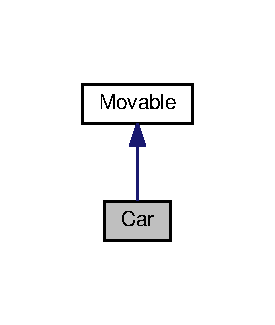
\includegraphics[width=132pt]{classCar__inherit__graph}
\end{center}
\end{figure}


Collaboration diagram for Car\-:
\nopagebreak
\begin{figure}[H]
\begin{center}
\leavevmode
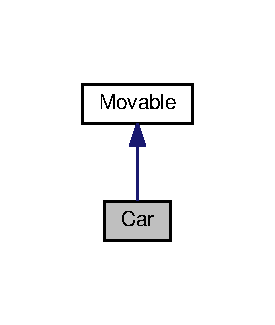
\includegraphics[width=132pt]{classCar__coll__graph}
\end{center}
\end{figure}
\subsection*{Static Public Member Functions}
\begin{DoxyCompactItemize}
\item 
static Ptr\-Car \hyperlink{classCar_a50ad84260f3062f98b0b61c59d98dca2}{create\-Car} (const \hyperlink{classPoint}{Point} \&start\-Point, const std\-::vector$<$ Ptr\-To\-Const\-Point $>$ \&points, const int speed, const unsigned int id)
\end{DoxyCompactItemize}
\subsection*{Additional Inherited Members}


\subsection{Detailed Description}
Represents car. \begin{DoxyAuthor}{Author}
Aleksander Brzozowski 
\end{DoxyAuthor}


\subsection{Member Function Documentation}
\hypertarget{classCar_a50ad84260f3062f98b0b61c59d98dca2}{\index{Car@{Car}!create\-Car@{create\-Car}}
\index{create\-Car@{create\-Car}!Car@{Car}}
\subsubsection[{create\-Car}]{\setlength{\rightskip}{0pt plus 5cm}Ptr\-Car Car\-::create\-Car (
\begin{DoxyParamCaption}
\item[{const {\bf Point} \&}]{start\-Point, }
\item[{const std\-::vector$<$ Ptr\-To\-Const\-Point $>$ \&}]{points, }
\item[{const int}]{speed, }
\item[{const unsigned int}]{id}
\end{DoxyParamCaption}
)\hspace{0.3cm}{\ttfamily [static]}}}\label{classCar_a50ad84260f3062f98b0b61c59d98dca2}
Constructs \hyperlink{classCar}{Car}. 
\begin{DoxyParams}{Parameters}
{\em start\-Point} & \hyperlink{classPoint}{Point} in which car will start \\
\hline
{\em points} & Points to follow by car \\
\hline
{\em speed} & \hyperlink{classCar}{Car}'s speed \\
\hline
{\em id} & \hyperlink{classCar}{Car}'s id \\
\hline
\end{DoxyParams}
\begin{DoxyReturn}{Returns}
Created car 
\end{DoxyReturn}


The documentation for this class was generated from the following files\-:\begin{DoxyCompactItemize}
\item 
/home/aleksander/\-C\-Lion\-Projects/\-Zpr/src/Movable.\-h\item 
/home/aleksander/\-C\-Lion\-Projects/\-Zpr/src/Movable.\-cpp\end{DoxyCompactItemize}

\hypertarget{classCarGUI}{\section{Car\-G\-U\-I Class Reference}
\label{classCarGUI}\index{Car\-G\-U\-I@{Car\-G\-U\-I}}
}


The \hyperlink{classCarGUI}{Car\-G\-U\-I} class.  




{\ttfamily \#include $<$cargui.\-h$>$}



Inheritance diagram for Car\-G\-U\-I\-:
\nopagebreak
\begin{figure}[H]
\begin{center}
\leavevmode
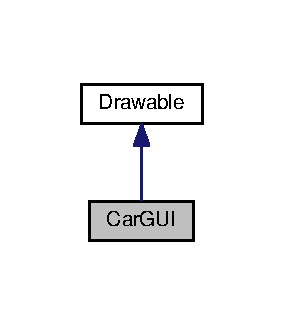
\includegraphics[width=136pt]{classCarGUI__inherit__graph}
\end{center}
\end{figure}


Collaboration diagram for Car\-G\-U\-I\-:
\nopagebreak
\begin{figure}[H]
\begin{center}
\leavevmode
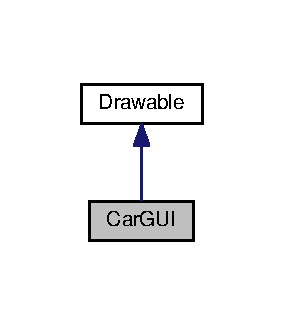
\includegraphics[width=136pt]{classCarGUI__coll__graph}
\end{center}
\end{figure}
\subsection*{Public Member Functions}
\begin{DoxyCompactItemize}
\item 
\hyperlink{classCarGUI_a3246f25cec9681b6719f41da2abaa21a}{Car\-G\-U\-I} (Q\-Rect car\-Rect, bool fast=false, bool ghost=false)
\begin{DoxyCompactList}\small\item\em \hyperlink{classCarGUI_a3246f25cec9681b6719f41da2abaa21a}{Car\-G\-U\-I\-::\-Car\-G\-U\-I}. \end{DoxyCompactList}\item 
\hyperlink{classCarGUI_a5b55f4b51094ca51114bd9e4f81b3981}{Car\-G\-U\-I} (unsigned int x, unsigned int y, bool fast=false, bool ghost=false)
\begin{DoxyCompactList}\small\item\em \hyperlink{classCarGUI_a3246f25cec9681b6719f41da2abaa21a}{Car\-G\-U\-I\-::\-Car\-G\-U\-I}. \end{DoxyCompactList}\item 
void \hyperlink{classCarGUI_afb151452fd5ab5723fbadc18b292b1cd}{draw} (Q\-Painter \&painter) const override
\begin{DoxyCompactList}\small\item\em \hyperlink{classCarGUI_afb151452fd5ab5723fbadc18b292b1cd}{Car\-G\-U\-I\-::draw}. \end{DoxyCompactList}\item 
void \hyperlink{classCarGUI_a9492214aed3b7bcdd9ac02a9d05c62c5}{set\-To} (unsigned int x, unsigned int y) override
\begin{DoxyCompactList}\small\item\em \hyperlink{classCarGUI_a9492214aed3b7bcdd9ac02a9d05c62c5}{Car\-G\-U\-I\-::set\-To}. \end{DoxyCompactList}\item 
bool \hyperlink{classCarGUI_ac10777d0be48432605fa02c7d1e70efc}{intersects} (Q\-Rect \&rectangle) const override
\begin{DoxyCompactList}\small\item\em \hyperlink{classCarGUI_ac10777d0be48432605fa02c7d1e70efc}{Car\-G\-U\-I\-::intersects}. \end{DoxyCompactList}\end{DoxyCompactItemize}
\subsection*{Static Public Attributes}
\begin{DoxyCompactItemize}
\item 
static const int \hyperlink{classCarGUI_a8d29447aca5b3c2e336aa65e95299e88}{W\-I\-D\-T\-H} = 10
\item 
\hypertarget{classCarGUI_aeca3f99b8146192a515ee78f787c3f9f}{static const int {\bfseries H\-E\-I\-G\-H\-T} = 10}\label{classCarGUI_aeca3f99b8146192a515ee78f787c3f9f}

\item 
\hypertarget{classCarGUI_abf7ae31a3d62b7ab4d76c21de1411c67}{static const int {\bfseries F\-A\-S\-T\-\_\-\-W\-I\-D\-T\-H} = 8}\label{classCarGUI_abf7ae31a3d62b7ab4d76c21de1411c67}

\item 
\hypertarget{classCarGUI_afd43e7040ed20f1d4ef5e1fc5bdf59d1}{static const int {\bfseries F\-A\-S\-T\-\_\-\-H\-E\-I\-G\-H\-T} = 8}\label{classCarGUI_afd43e7040ed20f1d4ef5e1fc5bdf59d1}

\item 
\hypertarget{classCarGUI_af56d7d01bc54b16ff78cc14cce570e10}{static const int {\bfseries P\-E\-N\-\_\-\-W\-I\-D\-T\-H} = 2}\label{classCarGUI_af56d7d01bc54b16ff78cc14cce570e10}

\item 
\hypertarget{classCarGUI_af14734c0d3a169cccf2ceca579201619}{static const Qt\-::\-Pen\-Style {\bfseries P\-E\-N\-\_\-\-S\-T\-Y\-L\-E} = Qt\-::\-Solid\-Line}\label{classCarGUI_af14734c0d3a169cccf2ceca579201619}

\item 
\hypertarget{classCarGUI_a8fc5e937a0c580cad858385de115b945}{static const Qt\-::\-Pen\-Cap\-Style {\bfseries P\-E\-N\-\_\-\-C\-A\-P} = Qt\-::\-Square\-Cap}\label{classCarGUI_a8fc5e937a0c580cad858385de115b945}

\item 
\hypertarget{classCarGUI_acb7a588f4fa762490d23d56324047b93}{static const Qt\-::\-Pen\-Join\-Style {\bfseries P\-E\-N\-\_\-\-J\-O\-I\-N} = Qt\-::\-Round\-Join}\label{classCarGUI_acb7a588f4fa762490d23d56324047b93}

\item 
\hypertarget{classCarGUI_afe262af5aff70256e0c4d3c5c2f6e48f}{static const Q\-Color {\bfseries P\-E\-N\-\_\-\-C\-O\-L\-O\-R} = Q\-Color(0, 0, 0)}\label{classCarGUI_afe262af5aff70256e0c4d3c5c2f6e48f}

\item 
\hypertarget{classCarGUI_acb446c6901b42114a46d8f1dc90f4688}{static const Q\-Color {\bfseries G\-H\-O\-S\-T\-\_\-\-P\-E\-N\-\_\-\-C\-O\-L\-O\-R} = Q\-Color(0, 0, 0, 127)}\label{classCarGUI_acb446c6901b42114a46d8f1dc90f4688}

\item 
\hypertarget{classCarGUI_a352bd9b2692ac49297643a854ffdb537}{static const Q\-Pen {\bfseries P\-E\-N}}\label{classCarGUI_a352bd9b2692ac49297643a854ffdb537}

\item 
\hypertarget{classCarGUI_a3ada4495d9bfecf7097aa3f42ad8756a}{static const Q\-Pen {\bfseries G\-H\-O\-S\-T\-\_\-\-P\-E\-N}}\label{classCarGUI_a3ada4495d9bfecf7097aa3f42ad8756a}

\item 
\hypertarget{classCarGUI_acc2a56343ab73144bca417ec16370c5c}{static const Qt\-::\-Brush\-Style {\bfseries B\-R\-U\-S\-H\-\_\-\-S\-T\-Y\-L\-E} = Qt\-::\-Solid\-Pattern}\label{classCarGUI_acc2a56343ab73144bca417ec16370c5c}

\item 
\hypertarget{classCarGUI_a9a50ecc06f437171f3961b5a671f01f1}{static const Q\-Color {\bfseries B\-R\-U\-S\-H\-\_\-\-C\-O\-L\-O\-R} = Q\-Color(27,133,184)}\label{classCarGUI_a9a50ecc06f437171f3961b5a671f01f1}

\item 
\hypertarget{classCarGUI_a0f2058112de433da200843c17e9c8e9e}{static const Q\-Color {\bfseries F\-A\-S\-T\-\_\-\-B\-R\-U\-S\-H\-\_\-\-C\-O\-L\-O\-R} = Q\-Color(119, 221, 119)}\label{classCarGUI_a0f2058112de433da200843c17e9c8e9e}

\item 
\hypertarget{classCarGUI_a4ba54f1295f2af07016f7a3a3e3fa6a7}{static const Q\-Color {\bfseries G\-H\-O\-S\-T\-\_\-\-B\-R\-U\-S\-H\-\_\-\-C\-O\-L\-O\-R} = Q\-Color(27,133,184, 127)}\label{classCarGUI_a4ba54f1295f2af07016f7a3a3e3fa6a7}

\item 
\hypertarget{classCarGUI_ab55f90d8af669b100b9cf262e6ff3e4c}{static const Q\-Color {\bfseries F\-A\-S\-T\-\_\-\-G\-H\-O\-S\-T\-\_\-\-B\-R\-U\-S\-H\-\_\-\-C\-O\-L\-O\-R} = Q\-Color(119, 221, 119, 127)}\label{classCarGUI_ab55f90d8af669b100b9cf262e6ff3e4c}

\item 
\hypertarget{classCarGUI_adb3513e5efe3da7e37ccf23879660697}{static const Q\-Brush {\bfseries B\-R\-U\-S\-H}}\label{classCarGUI_adb3513e5efe3da7e37ccf23879660697}

\item 
\hypertarget{classCarGUI_ad7c19970c7e76dcd5d81bd1d903aee03}{static const Q\-Brush {\bfseries F\-A\-S\-T\-\_\-\-B\-R\-U\-S\-H}}\label{classCarGUI_ad7c19970c7e76dcd5d81bd1d903aee03}

\item 
\hypertarget{classCarGUI_a40cb76f58891f02907dcdd4392747c81}{static const Q\-Brush {\bfseries G\-H\-O\-S\-T\-\_\-\-B\-R\-U\-S\-H}}\label{classCarGUI_a40cb76f58891f02907dcdd4392747c81}

\item 
\hypertarget{classCarGUI_aca0298de46fa045ffbb030fc060f1cae}{static const Q\-Brush {\bfseries F\-A\-S\-T\-\_\-\-G\-H\-O\-S\-T\-\_\-\-B\-R\-U\-S\-H}}\label{classCarGUI_aca0298de46fa045ffbb030fc060f1cae}

\item 
\hypertarget{classCarGUI_a435c3518e9bc11390e7f69c7da133d7a}{static const unsigned int {\bfseries C\-A\-R\-\_\-\-S\-P\-E\-E\-D} = 2}\label{classCarGUI_a435c3518e9bc11390e7f69c7da133d7a}

\item 
\hypertarget{classCarGUI_a8e8ec22f2116af401357e868d3d74b31}{static const unsigned int {\bfseries F\-A\-S\-T\-\_\-\-C\-A\-R\-\_\-\-S\-P\-E\-E\-D} = 3}\label{classCarGUI_a8e8ec22f2116af401357e868d3d74b31}

\end{DoxyCompactItemize}


\subsection{Detailed Description}
The \hyperlink{classCarGUI}{Car\-G\-U\-I} class. 

Class holds all necessary information to draw car object on screen. It implements functions from base class thar defines how car will look. It also holds all variables that define look of the both types of car object on screen. \begin{DoxyAuthor}{Author}
Pawel Rybak 
\end{DoxyAuthor}


\subsection{Constructor \& Destructor Documentation}
\hypertarget{classCarGUI_a3246f25cec9681b6719f41da2abaa21a}{\index{Car\-G\-U\-I@{Car\-G\-U\-I}!Car\-G\-U\-I@{Car\-G\-U\-I}}
\index{Car\-G\-U\-I@{Car\-G\-U\-I}!CarGUI@{Car\-G\-U\-I}}
\subsubsection[{Car\-G\-U\-I}]{\setlength{\rightskip}{0pt plus 5cm}Car\-G\-U\-I\-::\-Car\-G\-U\-I (
\begin{DoxyParamCaption}
\item[{Q\-Rect}]{car\-Rect, }
\item[{bool}]{fast = {\ttfamily false}, }
\item[{bool}]{ghost = {\ttfamily false}}
\end{DoxyParamCaption}
)}}\label{classCarGUI_a3246f25cec9681b6719f41da2abaa21a}


\hyperlink{classCarGUI_a3246f25cec9681b6719f41da2abaa21a}{Car\-G\-U\-I\-::\-Car\-G\-U\-I}. 


\begin{DoxyParams}{Parameters}
{\em car\-Rect} & -\/ Q\-Rect object on which car look is based. \\
\hline
{\em fast} & -\/ Bool flag whether car is fast car or not. \\
\hline
{\em ghost} & -\/ Bool flag whether object is ghost object or not.\\
\hline
\end{DoxyParams}
Constructs object based on Q\-Rect object given as argument. \hypertarget{classCarGUI_a5b55f4b51094ca51114bd9e4f81b3981}{\index{Car\-G\-U\-I@{Car\-G\-U\-I}!Car\-G\-U\-I@{Car\-G\-U\-I}}
\index{Car\-G\-U\-I@{Car\-G\-U\-I}!CarGUI@{Car\-G\-U\-I}}
\subsubsection[{Car\-G\-U\-I}]{\setlength{\rightskip}{0pt plus 5cm}Car\-G\-U\-I\-::\-Car\-G\-U\-I (
\begin{DoxyParamCaption}
\item[{unsigned int}]{x, }
\item[{unsigned int}]{y, }
\item[{bool}]{fast = {\ttfamily false}, }
\item[{bool}]{ghost = {\ttfamily false}}
\end{DoxyParamCaption}
)}}\label{classCarGUI_a5b55f4b51094ca51114bd9e4f81b3981}


\hyperlink{classCarGUI_a3246f25cec9681b6719f41da2abaa21a}{Car\-G\-U\-I\-::\-Car\-G\-U\-I}. 


\begin{DoxyParams}{Parameters}
{\em x} & -\/ Position X. \\
\hline
{\em y} & -\/ Position Y. \\
\hline
{\em fast} & -\/ Bool flag whether car is fast car or not. \\
\hline
{\em ghost} & -\/ Bool flag whether object is ghost object or not.\\
\hline
\end{DoxyParams}
Constructs object based on X and Y position given as arguments. Size of such car is defined in object fields. 

\subsection{Member Function Documentation}
\hypertarget{classCarGUI_afb151452fd5ab5723fbadc18b292b1cd}{\index{Car\-G\-U\-I@{Car\-G\-U\-I}!draw@{draw}}
\index{draw@{draw}!CarGUI@{Car\-G\-U\-I}}
\subsubsection[{draw}]{\setlength{\rightskip}{0pt plus 5cm}void Car\-G\-U\-I\-::draw (
\begin{DoxyParamCaption}
\item[{Q\-Painter \&}]{painter}
\end{DoxyParamCaption}
) const\hspace{0.3cm}{\ttfamily [override]}, {\ttfamily [virtual]}}}\label{classCarGUI_afb151452fd5ab5723fbadc18b292b1cd}


\hyperlink{classCarGUI_afb151452fd5ab5723fbadc18b292b1cd}{Car\-G\-U\-I\-::draw}. 


\begin{DoxyParams}{Parameters}
{\em painter} & -\/ Reference to painter object.\\
\hline
\end{DoxyParams}
Function draws object using painter given as an arrgument. It uses brushes and pens defined in object, and base its choice on whether object is ghost object or not. 

Implements \hyperlink{classDrawable}{Drawable}.

\hypertarget{classCarGUI_ac10777d0be48432605fa02c7d1e70efc}{\index{Car\-G\-U\-I@{Car\-G\-U\-I}!intersects@{intersects}}
\index{intersects@{intersects}!CarGUI@{Car\-G\-U\-I}}
\subsubsection[{intersects}]{\setlength{\rightskip}{0pt plus 5cm}bool Car\-G\-U\-I\-::intersects (
\begin{DoxyParamCaption}
\item[{Q\-Rect \&}]{rectangle}
\end{DoxyParamCaption}
) const\hspace{0.3cm}{\ttfamily [override]}, {\ttfamily [virtual]}}}\label{classCarGUI_ac10777d0be48432605fa02c7d1e70efc}


\hyperlink{classCarGUI_ac10777d0be48432605fa02c7d1e70efc}{Car\-G\-U\-I\-::intersects}. 


\begin{DoxyParams}{Parameters}
{\em rectangle} & -\/ Q\-Rect object that is being checked for intersection. \\
\hline
\end{DoxyParams}
\begin{DoxyReturn}{Returns}
Bool value whether rectangles intersects.
\end{DoxyReturn}
Function checks whether current object's rectangle and rectangle given as argument intersects and returns bool value. 

Implements \hyperlink{classDrawable}{Drawable}.

\hypertarget{classCarGUI_a9492214aed3b7bcdd9ac02a9d05c62c5}{\index{Car\-G\-U\-I@{Car\-G\-U\-I}!set\-To@{set\-To}}
\index{set\-To@{set\-To}!CarGUI@{Car\-G\-U\-I}}
\subsubsection[{set\-To}]{\setlength{\rightskip}{0pt plus 5cm}void Car\-G\-U\-I\-::set\-To (
\begin{DoxyParamCaption}
\item[{unsigned int}]{x, }
\item[{unsigned int}]{y}
\end{DoxyParamCaption}
)\hspace{0.3cm}{\ttfamily [override]}, {\ttfamily [virtual]}}}\label{classCarGUI_a9492214aed3b7bcdd9ac02a9d05c62c5}


\hyperlink{classCarGUI_a9492214aed3b7bcdd9ac02a9d05c62c5}{Car\-G\-U\-I\-::set\-To}. 


\begin{DoxyParams}{Parameters}
{\em x} & -\/ Position X. \\
\hline
{\em y} & -\/ Position Y.\\
\hline
\end{DoxyParams}
Function sets car object to position given as arguments. 

Implements \hyperlink{classDrawable}{Drawable}.



\subsection{Member Data Documentation}
\hypertarget{classCarGUI_a8d29447aca5b3c2e336aa65e95299e88}{\index{Car\-G\-U\-I@{Car\-G\-U\-I}!W\-I\-D\-T\-H@{W\-I\-D\-T\-H}}
\index{W\-I\-D\-T\-H@{W\-I\-D\-T\-H}!CarGUI@{Car\-G\-U\-I}}
\subsubsection[{W\-I\-D\-T\-H}]{\setlength{\rightskip}{0pt plus 5cm}const int Car\-G\-U\-I\-::\-W\-I\-D\-T\-H = 10\hspace{0.3cm}{\ttfamily [static]}}}\label{classCarGUI_a8d29447aca5b3c2e336aa65e95299e88}
P\-R\-O\-P\-E\-R\-T\-I\-E\-S

P\-R\-O\-P\-E\-R\-T\-I\-E\-S I\-N\-I\-T\-I\-A\-L\-I\-Z\-A\-T\-I\-O\-N 

The documentation for this class was generated from the following files\-:\begin{DoxyCompactItemize}
\item 
/home/aleksander/\-C\-Lion\-Projects/\-Zpr/src/\-G\-U\-I/cargui.\-h\item 
/home/aleksander/\-C\-Lion\-Projects/\-Zpr/src/\-G\-U\-I/cargui.\-cpp\end{DoxyCompactItemize}

\hypertarget{classCarRoute}{\section{Car\-Route Class Reference}
\label{classCarRoute}\index{Car\-Route@{Car\-Route}}
}


{\ttfamily \#include $<$Car\-Route.\-h$>$}



Inheritance diagram for Car\-Route\-:
\nopagebreak
\begin{figure}[H]
\begin{center}
\leavevmode
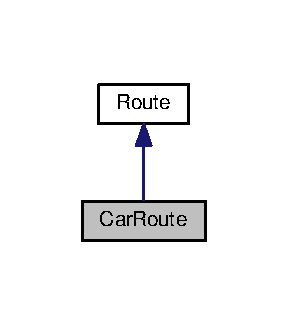
\includegraphics[width=138pt]{classCarRoute__inherit__graph}
\end{center}
\end{figure}


Collaboration diagram for Car\-Route\-:
\nopagebreak
\begin{figure}[H]
\begin{center}
\leavevmode
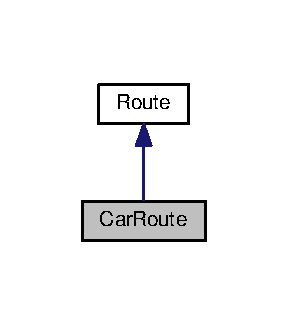
\includegraphics[width=138pt]{classCarRoute__coll__graph}
\end{center}
\end{figure}
\subsection*{Public Member Functions}
\begin{DoxyCompactItemize}
\item 
\hyperlink{classCarRoute_aa2fb96df759188781a2b534b533cf62b}{Car\-Route} (const std\-::vector$<$ Ptr\-To\-Const\-Point $>$ \&points)
\item 
bool \hyperlink{classCarRoute_a48a60e9054bcb3b775f4a56b50c0d79d}{next\-Point} () override
\item 
bool \hyperlink{classCarRoute_a4d8589aeb5b9accd189756dda8b618c6}{is\-End} () override
\end{DoxyCompactItemize}


\subsection{Detailed Description}
Represents route for car. \begin{DoxyAuthor}{Author}
Aleksander Brzozowski 
\end{DoxyAuthor}


\subsection{Constructor \& Destructor Documentation}
\hypertarget{classCarRoute_aa2fb96df759188781a2b534b533cf62b}{\index{Car\-Route@{Car\-Route}!Car\-Route@{Car\-Route}}
\index{Car\-Route@{Car\-Route}!CarRoute@{Car\-Route}}
\subsubsection[{Car\-Route}]{\setlength{\rightskip}{0pt plus 5cm}Car\-Route\-::\-Car\-Route (
\begin{DoxyParamCaption}
\item[{const std\-::vector$<$ Ptr\-To\-Const\-Point $>$ \&}]{points}
\end{DoxyParamCaption}
)}}\label{classCarRoute_aa2fb96df759188781a2b534b533cf62b}
Constructs \hyperlink{classHumanRoute}{Human\-Route}. 
\begin{DoxyParams}{Parameters}
{\em points} & Points to fallow by route \\
\hline
\end{DoxyParams}


\subsection{Member Function Documentation}
\hypertarget{classCarRoute_a4d8589aeb5b9accd189756dda8b618c6}{\index{Car\-Route@{Car\-Route}!is\-End@{is\-End}}
\index{is\-End@{is\-End}!CarRoute@{Car\-Route}}
\subsubsection[{is\-End}]{\setlength{\rightskip}{0pt plus 5cm}bool Car\-Route\-::is\-End (
\begin{DoxyParamCaption}
{}
\end{DoxyParamCaption}
)\hspace{0.3cm}{\ttfamily [override]}, {\ttfamily [virtual]}}}\label{classCarRoute_a4d8589aeb5b9accd189756dda8b618c6}
Checks is it end of \hyperlink{classRoute}{Route}. \begin{DoxyReturn}{Returns}
is end of \hyperlink{classRoute}{Route} 
\end{DoxyReturn}


Implements \hyperlink{classRoute_a0e1d104b56c768549f1b4fe4b575a6f5}{Route}.

\hypertarget{classCarRoute_a48a60e9054bcb3b775f4a56b50c0d79d}{\index{Car\-Route@{Car\-Route}!next\-Point@{next\-Point}}
\index{next\-Point@{next\-Point}!CarRoute@{Car\-Route}}
\subsubsection[{next\-Point}]{\setlength{\rightskip}{0pt plus 5cm}bool Car\-Route\-::next\-Point (
\begin{DoxyParamCaption}
{}
\end{DoxyParamCaption}
)\hspace{0.3cm}{\ttfamily [override]}, {\ttfamily [virtual]}}}\label{classCarRoute_a48a60e9054bcb3b775f4a56b50c0d79d}
Switches to the next point of route. \begin{DoxyReturn}{Returns}
Is next point of route 
\end{DoxyReturn}


Implements \hyperlink{classRoute_a27bb16170420801b5c191e9aea0134f1}{Route}.



The documentation for this class was generated from the following files\-:\begin{DoxyCompactItemize}
\item 
/home/aleksander/\-C\-Lion\-Projects/\-Zpr/src/Car\-Route.\-h\item 
/home/aleksander/\-C\-Lion\-Projects/\-Zpr/src/Car\-Route.\-cpp\end{DoxyCompactItemize}

\hypertarget{classCross}{\section{Cross Class Reference}
\label{classCross}\index{Cross@{Cross}}
}


\hyperlink{classCross}{Cross} represents vertices in the graph that describes map.  


\subsection*{Public Member Functions}
\begin{DoxyCompactItemize}
\item 
\hypertarget{classCross_a286bbd27e501b06c9989761815e4d150}{\hyperlink{classCross_a286bbd27e501b06c9989761815e4d150}{Cross} (Ptr\-To\-Const\-Point)}\label{classCross_a286bbd27e501b06c9989761815e4d150}

\begin{DoxyCompactList}\small\item\em Contructor for \hyperlink{classCross}{Cross}. \end{DoxyCompactList}\item 
Ptr\-Cross \hyperlink{classCross_a1e34c8d8207885c31fccc057e459eca0}{get\-Not\-Visited\-Neighbours} () const 
\begin{DoxyCompactList}\small\item\em Get this cross' neighbour that wasn't be used so far. \end{DoxyCompactList}\item 
void \hyperlink{classCross_a9a0803c662e8a9ebbeb25d2fb30b60d3}{add\-Neighbour} (Ptr\-Cross)
\begin{DoxyCompactList}\small\item\em Adding new neighbour and deciding if the new neighbour is on the north, east, west or south. \end{DoxyCompactList}\item 
bool \hyperlink{classCross_a707bf409f962936051ca4a35b086a1f6}{set\-Visited} (const bool \&)
\begin{DoxyCompactList}\small\item\em Changes the was\-Visited parameter by the finding route algorithm. \end{DoxyCompactList}\item 
\hypertarget{classCross_af04ae2fbefce9e2313e5cf172268635f}{bool {\bfseries get\-Visited} () const }\label{classCross_af04ae2fbefce9e2313e5cf172268635f}

\item 
\hypertarget{classCross_aa39b988d467b0d30ea71a7d2b3d36d43}{Ptr\-To\-Const\-Point {\bfseries get\-Position} () const }\label{classCross_aa39b988d467b0d30ea71a7d2b3d36d43}

\item 
\hypertarget{classCross_a25d38a1bcec3d88abfebed83e82cb133}{Ptr\-Cross {\bfseries get\-North\-Neighbour} () const }\label{classCross_a25d38a1bcec3d88abfebed83e82cb133}

\item 
\hypertarget{classCross_a1ddc074f996a3a36e2115be9c2b2aaf6}{Ptr\-Cross {\bfseries get\-South\-Neighbour} () const }\label{classCross_a1ddc074f996a3a36e2115be9c2b2aaf6}

\item 
\hypertarget{classCross_a8b83732b772b40341d5d08dad811f06a}{Ptr\-Cross {\bfseries get\-East\-Neighbour} () const }\label{classCross_a8b83732b772b40341d5d08dad811f06a}

\item 
\hypertarget{classCross_acec37a52c615de69566791de4d803fae}{Ptr\-Cross {\bfseries get\-West\-Neighbour} () const }\label{classCross_acec37a52c615de69566791de4d803fae}

\item 
bool \hyperlink{classCross_acf6cd8ddf999668bbd36a741902b72db}{operator==} (const \hyperlink{classCross}{Cross} \&rhs) const 
\item 
bool \hyperlink{classCross_a3895cda7b42236c090175a67cbd3f56c}{operator!=} (const \hyperlink{classCross}{Cross} \&rhs) const 
\end{DoxyCompactItemize}


\subsection{Detailed Description}
\hyperlink{classCross}{Cross} represents vertices in the graph that describes map. 

Each cross has it's neighbours and parameter that says if it was already used by the finding route algorithm and shouldn't be used again. 

\subsection{Member Function Documentation}
\hypertarget{classCross_a9a0803c662e8a9ebbeb25d2fb30b60d3}{\index{Cross@{Cross}!add\-Neighbour@{add\-Neighbour}}
\index{add\-Neighbour@{add\-Neighbour}!Cross@{Cross}}
\subsubsection[{add\-Neighbour}]{\setlength{\rightskip}{0pt plus 5cm}void Cross\-::add\-Neighbour (
\begin{DoxyParamCaption}
\item[{Ptr\-Cross}]{cr}
\end{DoxyParamCaption}
)}}\label{classCross_a9a0803c662e8a9ebbeb25d2fb30b60d3}


Adding new neighbour and deciding if the new neighbour is on the north, east, west or south. 


\begin{DoxyParams}{Parameters}
{\em cr} & -\/ new neighbour. \\
\hline
\end{DoxyParams}
\hypertarget{classCross_a1e34c8d8207885c31fccc057e459eca0}{\index{Cross@{Cross}!get\-Not\-Visited\-Neighbours@{get\-Not\-Visited\-Neighbours}}
\index{get\-Not\-Visited\-Neighbours@{get\-Not\-Visited\-Neighbours}!Cross@{Cross}}
\subsubsection[{get\-Not\-Visited\-Neighbours}]{\setlength{\rightskip}{0pt plus 5cm}Ptr\-Cross Cross\-::get\-Not\-Visited\-Neighbours (
\begin{DoxyParamCaption}
{}
\end{DoxyParamCaption}
) const}}\label{classCross_a1e34c8d8207885c31fccc057e459eca0}


Get this cross' neighbour that wasn't be used so far. 

\begin{DoxyReturn}{Returns}
not visited neighbour of this cross. 
\end{DoxyReturn}
\hypertarget{classCross_a3895cda7b42236c090175a67cbd3f56c}{\index{Cross@{Cross}!operator!=@{operator!=}}
\index{operator!=@{operator!=}!Cross@{Cross}}
\subsubsection[{operator!=}]{\setlength{\rightskip}{0pt plus 5cm}bool Cross\-::operator!= (
\begin{DoxyParamCaption}
\item[{const {\bf Cross} \&}]{rhs}
\end{DoxyParamCaption}
) const}}\label{classCross_a3895cda7b42236c090175a67cbd3f56c}
\begin{DoxyReturn}{Returns}
Returns true if two crosses have different positions. 
\end{DoxyReturn}
\hypertarget{classCross_acf6cd8ddf999668bbd36a741902b72db}{\index{Cross@{Cross}!operator==@{operator==}}
\index{operator==@{operator==}!Cross@{Cross}}
\subsubsection[{operator==}]{\setlength{\rightskip}{0pt plus 5cm}bool Cross\-::operator== (
\begin{DoxyParamCaption}
\item[{const {\bf Cross} \&}]{rhs}
\end{DoxyParamCaption}
) const}}\label{classCross_acf6cd8ddf999668bbd36a741902b72db}
\begin{DoxyReturn}{Returns}
Returns true if two crosses have the same position. 
\end{DoxyReturn}
\hypertarget{classCross_a707bf409f962936051ca4a35b086a1f6}{\index{Cross@{Cross}!set\-Visited@{set\-Visited}}
\index{set\-Visited@{set\-Visited}!Cross@{Cross}}
\subsubsection[{set\-Visited}]{\setlength{\rightskip}{0pt plus 5cm}bool Cross\-::set\-Visited (
\begin{DoxyParamCaption}
\item[{const bool \&}]{was\-Visited}
\end{DoxyParamCaption}
)}}\label{classCross_a707bf409f962936051ca4a35b086a1f6}


Changes the was\-Visited parameter by the finding route algorithm. 


\begin{DoxyParams}{Parameters}
{\em was\-Visited} & -\/ describes if the cross was used by the finding route algorithm and cannot be reused. \\
\hline
\end{DoxyParams}
\begin{DoxyReturn}{Returns}
the new value of was\-Visited parameter. 
\end{DoxyReturn}


The documentation for this class was generated from the following files\-:\begin{DoxyCompactItemize}
\item 
/home/aleksander/\-C\-Lion\-Projects/\-Zpr/src/\hyperlink{Cross_8h}{Cross.\-h}\item 
/home/aleksander/\-C\-Lion\-Projects/\-Zpr/src/\hyperlink{Cross_8cpp}{Cross.\-cpp}\end{DoxyCompactItemize}

\hypertarget{classCrossFactory}{\section{Cross\-Factory Class Reference}
\label{classCrossFactory}\index{Cross\-Factory@{Cross\-Factory}}
}


Factory creating crosses from given roads.  


\subsection*{Public Member Functions}
\begin{DoxyCompactItemize}
\item 
Ptr\-Cross \hyperlink{classCrossFactory_a20b57828696dfc9e8a2f3384d5d29bae}{find\-Cross\-By\-Point} (const Ptr\-To\-Const\-Point \&) const 
\begin{DoxyCompactList}\small\item\em Find the cross that has the same position as the given point as the argument. \end{DoxyCompactList}\item 
Ptr\-Cross \hyperlink{classCrossFactory_accdbbd63f5a76a62269e1dde580b72b7}{create\-New\-Cross} (const Ptr\-To\-Const\-Point \&)
\begin{DoxyCompactList}\small\item\em Creating new cross if it doesn't exist. \end{DoxyCompactList}\item 
void \hyperlink{classCrossFactory_aee15c59ec2656c5cc422a889c30d4581}{create\-Road} (const Ptr\-To\-Const\-Point \&, const Ptr\-To\-Const\-Point \&)
\begin{DoxyCompactList}\small\item\em Updating crosses, creating new crosses from the given road. \end{DoxyCompactList}\item 
void \hyperlink{classCrossFactory_ae8ac0c74d33e41161119e56e9995243e}{vert\-Crossed\-Road} (const Ptr\-To\-Const\-Point \&, const Ptr\-To\-Const\-Point \&)
\begin{DoxyCompactList}\small\item\em Updates crosses if new road crosses the existed one verticaly. \end{DoxyCompactList}\item 
void \hyperlink{classCrossFactory_ae1ea5359b31f09f76510c90e9b4552e5}{horiz\-Crossed\-Road} (const Ptr\-To\-Const\-Point \&, const Ptr\-To\-Const\-Point \&)
\begin{DoxyCompactList}\small\item\em Updates crosses if new road crosses the existed one horizontaly. \end{DoxyCompactList}\item 
void \hyperlink{classCrossFactory_aabc61b3a89fc71f7758780135c599e97}{two\-Horiz\-Roads} (const Ptr\-To\-Const\-Point \&, const Ptr\-To\-Const\-Point \&)
\begin{DoxyCompactList}\small\item\em Updates crosses if new road hide the existing, both roads are horizontaly. \end{DoxyCompactList}\item 
void \hyperlink{classCrossFactory_ac699978962ee263fb01c189891cb4a9b}{two\-Vert\-Roads} (const Ptr\-To\-Const\-Point \&, const Ptr\-To\-Const\-Point \&)
\begin{DoxyCompactList}\small\item\em Updates crosses if new road hide the existing, both roads are verticaly. \end{DoxyCompactList}\item 
\hypertarget{classCrossFactory_ae413173adae2b63cb79c6ac13aaa99d5}{std\-::vector$<$ Ptr\-Cross $>$ \& {\bfseries get\-Crosses} ()}\label{classCrossFactory_ae413173adae2b63cb79c6ac13aaa99d5}

\end{DoxyCompactItemize}
\subsection*{Static Public Member Functions}
\begin{DoxyCompactItemize}
\item 
static bool \hyperlink{classCrossFactory_a38f0b619437d1d866da32739aecb85eb}{cmp\-Cross\-X} (const Ptr\-Cross \&, const Ptr\-Cross \&)
\begin{DoxyCompactList}\small\item\em X value of cross position comparator for sorting. \end{DoxyCompactList}\item 
static bool \hyperlink{classCrossFactory_ac3f69512a614ed1f57c7595bd21f10c1}{cmp\-Cross\-Y} (const Ptr\-Cross \&, const Ptr\-Cross \&)
\begin{DoxyCompactList}\small\item\em Y value of cross position comparator for sorting. \end{DoxyCompactList}\end{DoxyCompactItemize}


\subsection{Detailed Description}
Factory creating crosses from given roads. 

Factory is able to create new crosses and update their neighbours. If new road crosses the road that already exists, new crosses at the crosses are created and neighbours are updated. 

\subsection{Member Function Documentation}
\hypertarget{classCrossFactory_a38f0b619437d1d866da32739aecb85eb}{\index{Cross\-Factory@{Cross\-Factory}!cmp\-Cross\-X@{cmp\-Cross\-X}}
\index{cmp\-Cross\-X@{cmp\-Cross\-X}!CrossFactory@{Cross\-Factory}}
\subsubsection[{cmp\-Cross\-X}]{\setlength{\rightskip}{0pt plus 5cm}bool Cross\-Factory\-::cmp\-Cross\-X (
\begin{DoxyParamCaption}
\item[{const Ptr\-Cross \&}]{cr1, }
\item[{const Ptr\-Cross \&}]{cr2}
\end{DoxyParamCaption}
)\hspace{0.3cm}{\ttfamily [static]}}}\label{classCrossFactory_a38f0b619437d1d866da32739aecb85eb}


X value of cross position comparator for sorting. 

Returns true if cross1 is nearer left. If both crosses have the same x, returns true if cross1 has smaller y than cross2. 
\begin{DoxyParams}{Parameters}
{\em cr1} & -\/ first cross. \\
\hline
{\em cr2} & -\/ second cross. \\
\hline
\end{DoxyParams}
\begin{DoxyReturn}{Returns}
true if x value of cross 1 is smaller than x value of cross 2, if both x values are the same, returns true if y value of cross 1 is smaller. 
\end{DoxyReturn}
\hypertarget{classCrossFactory_ac3f69512a614ed1f57c7595bd21f10c1}{\index{Cross\-Factory@{Cross\-Factory}!cmp\-Cross\-Y@{cmp\-Cross\-Y}}
\index{cmp\-Cross\-Y@{cmp\-Cross\-Y}!CrossFactory@{Cross\-Factory}}
\subsubsection[{cmp\-Cross\-Y}]{\setlength{\rightskip}{0pt plus 5cm}bool Cross\-Factory\-::cmp\-Cross\-Y (
\begin{DoxyParamCaption}
\item[{const Ptr\-Cross \&}]{cr1, }
\item[{const Ptr\-Cross \&}]{cr2}
\end{DoxyParamCaption}
)\hspace{0.3cm}{\ttfamily [static]}}}\label{classCrossFactory_ac3f69512a614ed1f57c7595bd21f10c1}


Y value of cross position comparator for sorting. 

Returns true if cross1 is nearer top. If both crosses have the same y, returns true if cross1 has smaller x than cross2. 
\begin{DoxyParams}{Parameters}
{\em cr1} & -\/ first cross. \\
\hline
{\em cr2} & -\/ second cross. \\
\hline
\end{DoxyParams}
\begin{DoxyReturn}{Returns}
true if y value of cross1 is smaller than y value of cross2, if both y values are the same, returns true if x value of cross1 is smaller. 
\end{DoxyReturn}
\hypertarget{classCrossFactory_accdbbd63f5a76a62269e1dde580b72b7}{\index{Cross\-Factory@{Cross\-Factory}!create\-New\-Cross@{create\-New\-Cross}}
\index{create\-New\-Cross@{create\-New\-Cross}!CrossFactory@{Cross\-Factory}}
\subsubsection[{create\-New\-Cross}]{\setlength{\rightskip}{0pt plus 5cm}Ptr\-Cross Cross\-Factory\-::create\-New\-Cross (
\begin{DoxyParamCaption}
\item[{const Ptr\-To\-Const\-Point \&}]{point}
\end{DoxyParamCaption}
)}}\label{classCrossFactory_accdbbd63f5a76a62269e1dde580b72b7}


Creating new cross if it doesn't exist. 

Checking if cross at given position already exists. If not creates new cross. 
\begin{DoxyParams}{Parameters}
{\em point} & -\/ point at which we want to create new cross. \\
\hline
\end{DoxyParams}
\begin{DoxyReturn}{Returns}
cross at given point. 
\end{DoxyReturn}
\hypertarget{classCrossFactory_aee15c59ec2656c5cc422a889c30d4581}{\index{Cross\-Factory@{Cross\-Factory}!create\-Road@{create\-Road}}
\index{create\-Road@{create\-Road}!CrossFactory@{Cross\-Factory}}
\subsubsection[{create\-Road}]{\setlength{\rightskip}{0pt plus 5cm}void Cross\-Factory\-::create\-Road (
\begin{DoxyParamCaption}
\item[{const Ptr\-To\-Const\-Point \&}]{begin, }
\item[{const Ptr\-To\-Const\-Point \&}]{end}
\end{DoxyParamCaption}
)}}\label{classCrossFactory_aee15c59ec2656c5cc422a889c30d4581}


Updating crosses, creating new crosses from the given road. 

Reverses the begin and ending point of the road if the ending point is nearer top left corner of the map. Then calls methods if the new road is horizontal or vertical. 
\begin{DoxyParams}{Parameters}
{\em begin} & -\/ starting point of the new road. \\
\hline
{\em end} & -\/ ending point of the new road. \\
\hline
\end{DoxyParams}
\hypertarget{classCrossFactory_a20b57828696dfc9e8a2f3384d5d29bae}{\index{Cross\-Factory@{Cross\-Factory}!find\-Cross\-By\-Point@{find\-Cross\-By\-Point}}
\index{find\-Cross\-By\-Point@{find\-Cross\-By\-Point}!CrossFactory@{Cross\-Factory}}
\subsubsection[{find\-Cross\-By\-Point}]{\setlength{\rightskip}{0pt plus 5cm}Ptr\-Cross Cross\-Factory\-::find\-Cross\-By\-Point (
\begin{DoxyParamCaption}
\item[{const Ptr\-To\-Const\-Point \&}]{point}
\end{DoxyParamCaption}
) const}}\label{classCrossFactory_a20b57828696dfc9e8a2f3384d5d29bae}


Find the cross that has the same position as the given point as the argument. 

Return cross that has the same position as given. 
\begin{DoxyParams}{Parameters}
{\em point} & -\/ given point to search. \\
\hline
\end{DoxyParams}
\begin{DoxyReturn}{Returns}
cross that has the same point as given. 
\end{DoxyReturn}
\hypertarget{classCrossFactory_ae1ea5359b31f09f76510c90e9b4552e5}{\index{Cross\-Factory@{Cross\-Factory}!horiz\-Crossed\-Road@{horiz\-Crossed\-Road}}
\index{horiz\-Crossed\-Road@{horiz\-Crossed\-Road}!CrossFactory@{Cross\-Factory}}
\subsubsection[{horiz\-Crossed\-Road}]{\setlength{\rightskip}{0pt plus 5cm}void Cross\-Factory\-::horiz\-Crossed\-Road (
\begin{DoxyParamCaption}
\item[{const Ptr\-To\-Const\-Point \&}]{begin, }
\item[{const Ptr\-To\-Const\-Point \&}]{end}
\end{DoxyParamCaption}
)}}\label{classCrossFactory_ae1ea5359b31f09f76510c90e9b4552e5}


Updates crosses if new road crosses the existed one horizontaly. 

This method creates new crosses if the new road crosses with the another roads. The new road is horizontal. At first, crosses are sorted. The first is cross that has the smallest x value of the position. Then we check each pair of cross and it's south neighbour, if the new road doesn't cross the road between these pair of crosses. If it crosses, new crosses are added and neighbours are updated. 
\begin{DoxyParams}{Parameters}
{\em begin} & -\/ point on the west of the new road. \\
\hline
{\em end} & -\/ point on the east of the new road. \\
\hline
\end{DoxyParams}
\hypertarget{classCrossFactory_aabc61b3a89fc71f7758780135c599e97}{\index{Cross\-Factory@{Cross\-Factory}!two\-Horiz\-Roads@{two\-Horiz\-Roads}}
\index{two\-Horiz\-Roads@{two\-Horiz\-Roads}!CrossFactory@{Cross\-Factory}}
\subsubsection[{two\-Horiz\-Roads}]{\setlength{\rightskip}{0pt plus 5cm}void Cross\-Factory\-::two\-Horiz\-Roads (
\begin{DoxyParamCaption}
\item[{const Ptr\-To\-Const\-Point \&}]{begin, }
\item[{const Ptr\-To\-Const\-Point \&}]{end}
\end{DoxyParamCaption}
)}}\label{classCrossFactory_aabc61b3a89fc71f7758780135c599e97}


Updates crosses if new road hide the existing, both roads are horizontaly. 

Check if two roads are horizontal and both of roads have the same y value. (If one road hides another road). At first crosses are sorted. First cross should has the smallest y value of the position. Then we look for the two crosses, between which the new road is being tried to set. If found, we create new crosses and update neighbours from the west to the east. 
\begin{DoxyParams}{Parameters}
{\em begin} & -\/ point on the west of the new road. \\
\hline
{\em end} & -\/ point on the east of the new road. \\
\hline
\end{DoxyParams}
\hypertarget{classCrossFactory_ac699978962ee263fb01c189891cb4a9b}{\index{Cross\-Factory@{Cross\-Factory}!two\-Vert\-Roads@{two\-Vert\-Roads}}
\index{two\-Vert\-Roads@{two\-Vert\-Roads}!CrossFactory@{Cross\-Factory}}
\subsubsection[{two\-Vert\-Roads}]{\setlength{\rightskip}{0pt plus 5cm}void Cross\-Factory\-::two\-Vert\-Roads (
\begin{DoxyParamCaption}
\item[{const Ptr\-To\-Const\-Point \&}]{begin, }
\item[{const Ptr\-To\-Const\-Point \&}]{end}
\end{DoxyParamCaption}
)}}\label{classCrossFactory_ac699978962ee263fb01c189891cb4a9b}


Updates crosses if new road hide the existing, both roads are verticaly. 

Check if two roads are vertical and both of roads have the same x value. (If one road hides another road). At first crosses are sorted. First cross should has the smallest x value of the position Then we look for the two crosses, between which the new road is being tried to set. If found, we create new crosses and update neighbours from the north to the south. 
\begin{DoxyParams}{Parameters}
{\em begin} & -\/ point on the north of the new road. \\
\hline
{\em end} & -\/ point on the south of the new road. \\
\hline
\end{DoxyParams}
\hypertarget{classCrossFactory_ae8ac0c74d33e41161119e56e9995243e}{\index{Cross\-Factory@{Cross\-Factory}!vert\-Crossed\-Road@{vert\-Crossed\-Road}}
\index{vert\-Crossed\-Road@{vert\-Crossed\-Road}!CrossFactory@{Cross\-Factory}}
\subsubsection[{vert\-Crossed\-Road}]{\setlength{\rightskip}{0pt plus 5cm}void Cross\-Factory\-::vert\-Crossed\-Road (
\begin{DoxyParamCaption}
\item[{const Ptr\-To\-Const\-Point \&}]{begin, }
\item[{const Ptr\-To\-Const\-Point \&}]{end}
\end{DoxyParamCaption}
)}}\label{classCrossFactory_ae8ac0c74d33e41161119e56e9995243e}


Updates crosses if new road crosses the existed one verticaly. 

This method creates new crosses if the new road crosses with the another roads. The new road is vertical. At first, crosses are sorted. The first is cross that has the smallest y value of the position. Then we check each pair of cross and it's east neighbour, if the new road doesn't cross the road between these pair of crosses. If it crosses, new crosses are added and neighbours are updated. 
\begin{DoxyParams}{Parameters}
{\em begin} & -\/ point on the north of the new road. \\
\hline
{\em end} & -\/ point on the south of the new road. \\
\hline
\end{DoxyParams}


The documentation for this class was generated from the following files\-:\begin{DoxyCompactItemize}
\item 
/home/aleksander/\-C\-Lion\-Projects/\-Zpr/src/\hyperlink{CrossFactory_8h}{Cross\-Factory.\-h}\item 
/home/aleksander/\-C\-Lion\-Projects/\-Zpr/src/\hyperlink{CrossFactory_8cpp}{Cross\-Factory.\-cpp}\end{DoxyCompactItemize}

\hypertarget{classCrossFactoryTest}{\section{Cross\-Factory\-Test Class Reference}
\label{classCrossFactoryTest}\index{Cross\-Factory\-Test@{Cross\-Factory\-Test}}
}


Inheritance diagram for Cross\-Factory\-Test\-:
\nopagebreak
\begin{figure}[H]
\begin{center}
\leavevmode
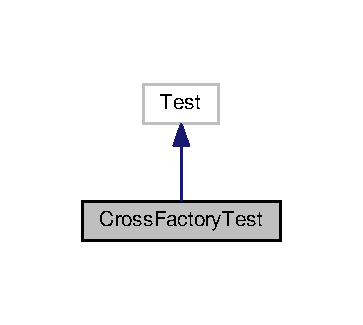
\includegraphics[width=174pt]{classCrossFactoryTest__inherit__graph}
\end{center}
\end{figure}


Collaboration diagram for Cross\-Factory\-Test\-:
\nopagebreak
\begin{figure}[H]
\begin{center}
\leavevmode
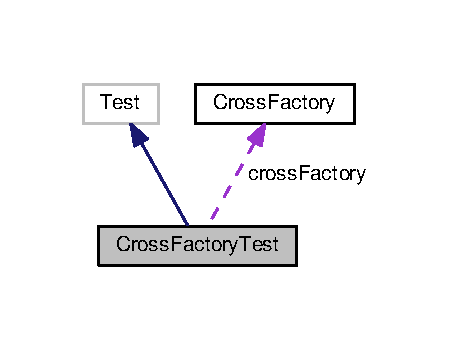
\includegraphics[width=217pt]{classCrossFactoryTest__coll__graph}
\end{center}
\end{figure}
\subsection*{Public Member Functions}
\begin{DoxyCompactItemize}
\item 
\hypertarget{classCrossFactoryTest_a9c2960a7cdf153afc8fbec7e759fdaa5}{void {\bfseries create\-Route} (Ptr\-To\-Const\-Point src, Ptr\-To\-Const\-Point dst)}\label{classCrossFactoryTest_a9c2960a7cdf153afc8fbec7e759fdaa5}

\item 
\hypertarget{classCrossFactoryTest_af82d127713574f5f962f3774206dddf0}{void {\bfseries create\-Crosses} ()}\label{classCrossFactoryTest_af82d127713574f5f962f3774206dddf0}

\item 
\hypertarget{classCrossFactoryTest_af3f6b63f273493a5c354243ff713fe74}{void {\bfseries create\-More\-Crosses} ()}\label{classCrossFactoryTest_af3f6b63f273493a5c354243ff713fe74}

\end{DoxyCompactItemize}
\subsection*{Public Attributes}
\begin{DoxyCompactItemize}
\item 
\hypertarget{classCrossFactoryTest_a4f8d430683d98c9ef9b190346c136935}{\hyperlink{classCrossFactory}{Cross\-Factory} {\bfseries cross\-Factory}}\label{classCrossFactoryTest_a4f8d430683d98c9ef9b190346c136935}

\end{DoxyCompactItemize}


The documentation for this class was generated from the following file\-:\begin{DoxyCompactItemize}
\item 
/home/aleksander/\-C\-Lion\-Projects/\-Zpr/test/Cross\-Factory\-Test.\-cpp\end{DoxyCompactItemize}

\hypertarget{classCrossTest}{\section{Cross\-Test Class Reference}
\label{classCrossTest}\index{Cross\-Test@{Cross\-Test}}
}


Inheritance diagram for Cross\-Test\-:
\nopagebreak
\begin{figure}[H]
\begin{center}
\leavevmode
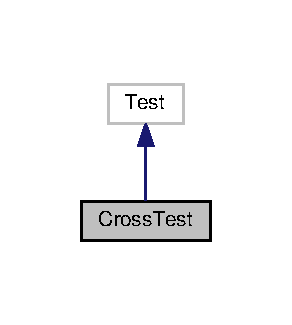
\includegraphics[width=140pt]{classCrossTest__inherit__graph}
\end{center}
\end{figure}


Collaboration diagram for Cross\-Test\-:
\nopagebreak
\begin{figure}[H]
\begin{center}
\leavevmode
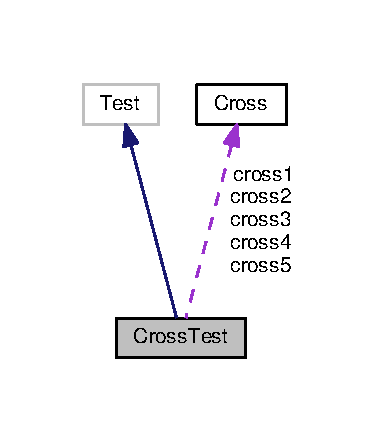
\includegraphics[width=182pt]{classCrossTest__coll__graph}
\end{center}
\end{figure}
\subsection*{Public Member Functions}
\begin{DoxyCompactItemize}
\item 
\hypertarget{classCrossTest_a36c8b9516a0ecde4b7caad5524c60c2d}{void {\bfseries make\-\_\-neighbours} ()}\label{classCrossTest_a36c8b9516a0ecde4b7caad5524c60c2d}

\end{DoxyCompactItemize}
\subsection*{Public Attributes}
\begin{DoxyCompactItemize}
\item 
\hypertarget{classCrossTest_af2f3d52c7440ac3e6223c75e125182ad}{\hyperlink{classCross}{Cross} $\ast$ {\bfseries cross1}}\label{classCrossTest_af2f3d52c7440ac3e6223c75e125182ad}

\item 
\hypertarget{classCrossTest_a2c4c65790a9116cfa2ead593caee515a}{\hyperlink{classCross}{Cross} $\ast$ {\bfseries cross2}}\label{classCrossTest_a2c4c65790a9116cfa2ead593caee515a}

\item 
\hypertarget{classCrossTest_ae43298a5b19936b1fad6d50664ec2eac}{\hyperlink{classCross}{Cross} $\ast$ {\bfseries cross3}}\label{classCrossTest_ae43298a5b19936b1fad6d50664ec2eac}

\item 
\hypertarget{classCrossTest_a4b61562083e4c5e44c21f49b2b62ba65}{\hyperlink{classCross}{Cross} $\ast$ {\bfseries cross4}}\label{classCrossTest_a4b61562083e4c5e44c21f49b2b62ba65}

\item 
\hypertarget{classCrossTest_aee9ea5edcf55f7f8b1fde08f40db3b17}{\hyperlink{classCross}{Cross} $\ast$ {\bfseries cross5}}\label{classCrossTest_aee9ea5edcf55f7f8b1fde08f40db3b17}

\end{DoxyCompactItemize}


The documentation for this class was generated from the following file\-:\begin{DoxyCompactItemize}
\item 
/home/aleksander/\-C\-Lion\-Projects/\-Zpr/test/Cross\-Test.\-cpp\end{DoxyCompactItemize}

\hypertarget{classDrawable}{\section{Drawable Class Reference}
\label{classDrawable}\index{Drawable@{Drawable}}
}


The \hyperlink{classDrawable}{Drawable} class.  




{\ttfamily \#include $<$drawable.\-h$>$}



Inheritance diagram for Drawable\-:
\nopagebreak
\begin{figure}[H]
\begin{center}
\leavevmode
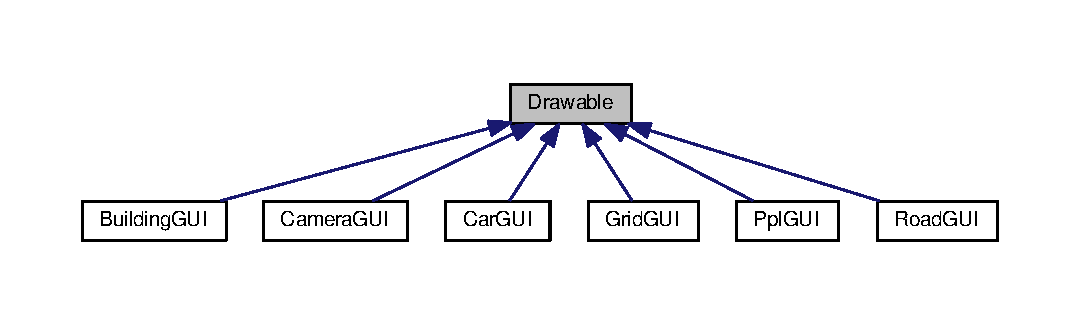
\includegraphics[width=350pt]{classDrawable__inherit__graph}
\end{center}
\end{figure}
\subsection*{Public Member Functions}
\begin{DoxyCompactItemize}
\item 
\hyperlink{classDrawable_af63902e4fe7ec2aef7ad56eec0168822}{Drawable} (bool)
\begin{DoxyCompactList}\small\item\em \hyperlink{classDrawable_af63902e4fe7ec2aef7ad56eec0168822}{Drawable\-::\-Drawable}. Constructor. \end{DoxyCompactList}\item 
\hypertarget{classDrawable_abf4d2776b43b2bd93710591926587934}{virtual \hyperlink{classDrawable_abf4d2776b43b2bd93710591926587934}{$\sim$\-Drawable} ()=0}\label{classDrawable_abf4d2776b43b2bd93710591926587934}

\begin{DoxyCompactList}\small\item\em \hyperlink{classDrawable_abf4d2776b43b2bd93710591926587934}{Drawable\-::$\sim$\-Drawable}. Virtual destructor. \end{DoxyCompactList}\item 
\hypertarget{classDrawable_ab5e74918b6cf0149cb192b9ec56556c1}{virtual void {\bfseries draw} (Q\-Painter \&) const =0}\label{classDrawable_ab5e74918b6cf0149cb192b9ec56556c1}

\item 
\hypertarget{classDrawable_a8fa095e72a5b0a60488ac977bf77a34b}{virtual void {\bfseries set\-To} (unsigned int x, unsigned int y)=0}\label{classDrawable_a8fa095e72a5b0a60488ac977bf77a34b}

\item 
\hypertarget{classDrawable_a81d6ed7b86df48ec36e731b377b066cf}{virtual bool {\bfseries intersects} (Q\-Rect \&rectangle) const =0}\label{classDrawable_a81d6ed7b86df48ec36e731b377b066cf}

\item 
bool \hyperlink{classDrawable_a631734def2897ecb976b725a5d4fd554}{is\-Ghost} () const 
\begin{DoxyCompactList}\small\item\em \hyperlink{classDrawable_a631734def2897ecb976b725a5d4fd554}{Drawable\-::is\-Ghost}. \end{DoxyCompactList}\end{DoxyCompactItemize}


\subsection{Detailed Description}
The \hyperlink{classDrawable}{Drawable} class. 

Base class for all the objects that represents objects drawn on screen. It has three purely virtual classes that needs to be implemented. Its main purpouse is to create common interface of drawing all objects that can be drawn. \begin{DoxyAuthor}{Author}
Pawel Rybak 
\end{DoxyAuthor}


\subsection{Constructor \& Destructor Documentation}
\hypertarget{classDrawable_af63902e4fe7ec2aef7ad56eec0168822}{\index{Drawable@{Drawable}!Drawable@{Drawable}}
\index{Drawable@{Drawable}!Drawable@{Drawable}}
\subsubsection[{Drawable}]{\setlength{\rightskip}{0pt plus 5cm}Drawable\-::\-Drawable (
\begin{DoxyParamCaption}
\item[{bool}]{ghost = {\ttfamily false}}
\end{DoxyParamCaption}
)}}\label{classDrawable_af63902e4fe7ec2aef7ad56eec0168822}


\hyperlink{classDrawable_af63902e4fe7ec2aef7ad56eec0168822}{Drawable\-::\-Drawable}. Constructor. 


\begin{DoxyParams}{Parameters}
{\em ghost} & -\/ bool flag tells whether object is ghost object. \\
\hline
\end{DoxyParams}


\subsection{Member Function Documentation}
\hypertarget{classDrawable_a631734def2897ecb976b725a5d4fd554}{\index{Drawable@{Drawable}!is\-Ghost@{is\-Ghost}}
\index{is\-Ghost@{is\-Ghost}!Drawable@{Drawable}}
\subsubsection[{is\-Ghost}]{\setlength{\rightskip}{0pt plus 5cm}bool Drawable\-::is\-Ghost (
\begin{DoxyParamCaption}
{}
\end{DoxyParamCaption}
) const}}\label{classDrawable_a631734def2897ecb976b725a5d4fd554}


\hyperlink{classDrawable_a631734def2897ecb976b725a5d4fd554}{Drawable\-::is\-Ghost}. 

\begin{DoxyReturn}{Returns}
boolean whether object is ghost object. 
\end{DoxyReturn}


The documentation for this class was generated from the following files\-:\begin{DoxyCompactItemize}
\item 
/home/aleksander/\-C\-Lion\-Projects/\-Zpr/src/\-G\-U\-I/drawable.\-h\item 
/home/aleksander/\-C\-Lion\-Projects/\-Zpr/src/\-G\-U\-I/drawable.\-cpp\end{DoxyCompactItemize}

\hypertarget{classEventInterpreter}{\section{Event\-Interpreter Class Reference}
\label{classEventInterpreter}\index{Event\-Interpreter@{Event\-Interpreter}}
}


The \hyperlink{classEventInterpreter}{Event\-Interpreter} class.  




{\ttfamily \#include $<$eventinterpreter.\-h$>$}



Inheritance diagram for Event\-Interpreter\-:
\nopagebreak
\begin{figure}[H]
\begin{center}
\leavevmode
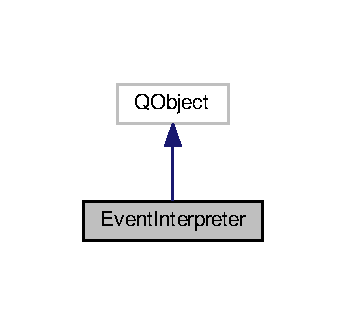
\includegraphics[width=166pt]{classEventInterpreter__inherit__graph}
\end{center}
\end{figure}


Collaboration diagram for Event\-Interpreter\-:
\nopagebreak
\begin{figure}[H]
\begin{center}
\leavevmode
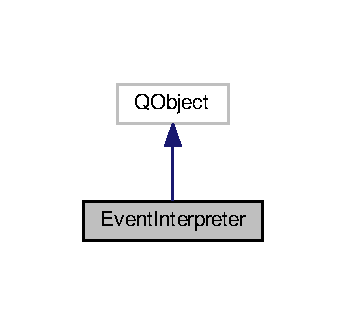
\includegraphics[width=166pt]{classEventInterpreter__coll__graph}
\end{center}
\end{figure}
\subsection*{Public Types}
\begin{DoxyCompactItemize}
\item 
enum \hyperlink{classEventInterpreter_a1b63d40701a33e256a8cbbf44c6be8d2}{Option} \{ \\*
{\bfseries set\-Road}, 
{\bfseries set\-Car}, 
{\bfseries set\-Fast\-Car}, 
{\bfseries set\-Building}, 
\\*
{\bfseries set\-Camera}, 
{\bfseries set\-Human}, 
{\bfseries do\-Nothing}
 \}
\begin{DoxyCompactList}\small\item\em The Option enum. \end{DoxyCompactList}\end{DoxyCompactItemize}
\subsection*{Signals}
\begin{DoxyCompactItemize}
\item 
\hypertarget{classEventInterpreter_a58713917f8a69790e37a7f6b7c507876}{void {\bfseries road\-Created} (\hyperlink{classRoadGUI}{Road\-G\-U\-I} $\ast$)}\label{classEventInterpreter_a58713917f8a69790e37a7f6b7c507876}

\item 
\hypertarget{classEventInterpreter_a0920b5e9443c614e443b65a853d5e7f1}{void {\bfseries drawable\-Created} (\hyperlink{classDrawable}{Drawable} $\ast$)}\label{classEventInterpreter_a0920b5e9443c614e443b65a853d5e7f1}

\item 
\hypertarget{classEventInterpreter_a737c2f2f409b24fe35f8aab0e07af7dc}{void {\bfseries camera\-Created} (\hyperlink{classCameraGUI}{Camera\-G\-U\-I} $\ast$)}\label{classEventInterpreter_a737c2f2f409b24fe35f8aab0e07af7dc}

\end{DoxyCompactItemize}
\subsection*{Public Member Functions}
\begin{DoxyCompactItemize}
\item 
\hyperlink{classEventInterpreter_ada70531370606873ff55e29a923a9096}{Event\-Interpreter} ()
\begin{DoxyCompactList}\small\item\em \hyperlink{classEventInterpreter_ada70531370606873ff55e29a923a9096}{Event\-Interpreter\-::\-Event\-Interpreter}. \end{DoxyCompactList}\item 
void \hyperlink{classEventInterpreter_ad99704356fcdfbaa5982e463a6a27318}{mouse\-Moved} (int x, int y)
\begin{DoxyCompactList}\small\item\em \hyperlink{classEventInterpreter_ad99704356fcdfbaa5982e463a6a27318}{Event\-Interpreter\-::mouse\-Moved}. \end{DoxyCompactList}\item 
void \hyperlink{classEventInterpreter_a74690162262290d519369630015f6cef}{mouse\-Clicked} (int x, int y)
\begin{DoxyCompactList}\small\item\em \hyperlink{classEventInterpreter_a74690162262290d519369630015f6cef}{Event\-Interpreter\-::mouse\-Clicked}. \end{DoxyCompactList}\item 
\hypertarget{classEventInterpreter_aa977815c55a5eb97577aa5d1e73379cb}{void {\bfseries steer\-Camera} (int key\-Code)}\label{classEventInterpreter_aa977815c55a5eb97577aa5d1e73379cb}

\item 
void \hyperlink{classEventInterpreter_a6ca1d621b8ef0297675be928b996ae8b}{set\-Map} (std\-::shared\-\_\-ptr$<$ \hyperlink{classMap}{Map} $>$ map)
\begin{DoxyCompactList}\small\item\em \hyperlink{classEventInterpreter_a6ca1d621b8ef0297675be928b996ae8b}{Event\-Interpreter\-::set\-Map}. \end{DoxyCompactList}\item 
void \hyperlink{classEventInterpreter_ae5b4f14200e6ce7202852306194ee767}{snap\-To\-Grid\-Center} (\hyperlink{classPoint}{Point} \&point) const 
\begin{DoxyCompactList}\small\item\em \hyperlink{classEventInterpreter_ae5b4f14200e6ce7202852306194ee767}{Event\-Interpreter\-::snap\-To\-Grid\-Center}. \end{DoxyCompactList}\item 
void \hyperlink{classEventInterpreter_a538d5fd0db5b5ffccb72381d889970a8}{snap\-To\-Grid\-Intersect} (\hyperlink{classPoint}{Point} \&point) const 
\begin{DoxyCompactList}\small\item\em \hyperlink{classEventInterpreter_a538d5fd0db5b5ffccb72381d889970a8}{Event\-Interpreter\-::snap\-To\-Grid\-Intersect}. \end{DoxyCompactList}\item 
std\-::shared\-\_\-ptr$<$ \hyperlink{classDrawable}{Drawable} $>$ \hyperlink{classEventInterpreter_aba8f008c996f9f73b5d3420ff1231869}{set\-Current\-Option} (\hyperlink{classEventInterpreter_a1b63d40701a33e256a8cbbf44c6be8d2}{Option} option)
\begin{DoxyCompactList}\small\item\em \hyperlink{classEventInterpreter_aba8f008c996f9f73b5d3420ff1231869}{Event\-Interpreter\-::set\-Current\-Option}. \end{DoxyCompactList}\item 
\hyperlink{classEventInterpreter_a1b63d40701a33e256a8cbbf44c6be8d2}{Option} \hyperlink{classEventInterpreter_a9caa73a223dcaa65d1ec6e06398d9b61}{get\-Current\-Option} ()
\begin{DoxyCompactList}\small\item\em \hyperlink{classEventInterpreter_a9caa73a223dcaa65d1ec6e06398d9b61}{Event\-Interpreter\-::get\-Current\-Option}. \end{DoxyCompactList}\end{DoxyCompactItemize}


\subsection{Detailed Description}
The \hyperlink{classEventInterpreter}{Event\-Interpreter} class. 

Object responsible for interpretating user input. It has field that remebers current tool chosen by user and using that can interpret maouse and keyboard events properly. 

\subsection{Member Enumeration Documentation}
\hypertarget{classEventInterpreter_a1b63d40701a33e256a8cbbf44c6be8d2}{\index{Event\-Interpreter@{Event\-Interpreter}!Option@{Option}}
\index{Option@{Option}!EventInterpreter@{Event\-Interpreter}}
\subsubsection[{Option}]{\setlength{\rightskip}{0pt plus 5cm}enum {\bf Event\-Interpreter\-::\-Option}\hspace{0.3cm}{\ttfamily [strong]}}}\label{classEventInterpreter_a1b63d40701a33e256a8cbbf44c6be8d2}


The Option enum. 

Enum class describing current tool. 

\subsection{Constructor \& Destructor Documentation}
\hypertarget{classEventInterpreter_ada70531370606873ff55e29a923a9096}{\index{Event\-Interpreter@{Event\-Interpreter}!Event\-Interpreter@{Event\-Interpreter}}
\index{Event\-Interpreter@{Event\-Interpreter}!EventInterpreter@{Event\-Interpreter}}
\subsubsection[{Event\-Interpreter}]{\setlength{\rightskip}{0pt plus 5cm}Event\-Interpreter\-::\-Event\-Interpreter (
\begin{DoxyParamCaption}
{}
\end{DoxyParamCaption}
)}}\label{classEventInterpreter_ada70531370606873ff55e29a923a9096}


\hyperlink{classEventInterpreter_ada70531370606873ff55e29a923a9096}{Event\-Interpreter\-::\-Event\-Interpreter}. 

Constructor. Initiats object's fields. 

\subsection{Member Function Documentation}
\hypertarget{classEventInterpreter_a9caa73a223dcaa65d1ec6e06398d9b61}{\index{Event\-Interpreter@{Event\-Interpreter}!get\-Current\-Option@{get\-Current\-Option}}
\index{get\-Current\-Option@{get\-Current\-Option}!EventInterpreter@{Event\-Interpreter}}
\subsubsection[{get\-Current\-Option}]{\setlength{\rightskip}{0pt plus 5cm}{\bf Event\-Interpreter\-::\-Option} Event\-Interpreter\-::get\-Current\-Option (
\begin{DoxyParamCaption}
{}
\end{DoxyParamCaption}
)}}\label{classEventInterpreter_a9caa73a223dcaa65d1ec6e06398d9b61}


\hyperlink{classEventInterpreter_a9caa73a223dcaa65d1ec6e06398d9b61}{Event\-Interpreter\-::get\-Current\-Option}. 

\begin{DoxyReturn}{Returns}
Returns current option. 
\end{DoxyReturn}
\hypertarget{classEventInterpreter_a74690162262290d519369630015f6cef}{\index{Event\-Interpreter@{Event\-Interpreter}!mouse\-Clicked@{mouse\-Clicked}}
\index{mouse\-Clicked@{mouse\-Clicked}!EventInterpreter@{Event\-Interpreter}}
\subsubsection[{mouse\-Clicked}]{\setlength{\rightskip}{0pt plus 5cm}void Event\-Interpreter\-::mouse\-Clicked (
\begin{DoxyParamCaption}
\item[{int}]{x, }
\item[{int}]{y}
\end{DoxyParamCaption}
)}}\label{classEventInterpreter_a74690162262290d519369630015f6cef}


\hyperlink{classEventInterpreter_a74690162262290d519369630015f6cef}{Event\-Interpreter\-::mouse\-Clicked}. 


\begin{DoxyParams}{Parameters}
{\em x} & -\/ mouse position X. \\
\hline
{\em y} & -\/ mouse position Y.\\
\hline
\end{DoxyParams}
Interprets mouse click events. It is based on current option and whether anchor point is valid. Unless current tool needs only one point to be created, first click sets anchor field, and second calls function to construct object that takes two points in constructor. \hypertarget{classEventInterpreter_ad99704356fcdfbaa5982e463a6a27318}{\index{Event\-Interpreter@{Event\-Interpreter}!mouse\-Moved@{mouse\-Moved}}
\index{mouse\-Moved@{mouse\-Moved}!EventInterpreter@{Event\-Interpreter}}
\subsubsection[{mouse\-Moved}]{\setlength{\rightskip}{0pt plus 5cm}void Event\-Interpreter\-::mouse\-Moved (
\begin{DoxyParamCaption}
\item[{int}]{x, }
\item[{int}]{y}
\end{DoxyParamCaption}
)}}\label{classEventInterpreter_ad99704356fcdfbaa5982e463a6a27318}


\hyperlink{classEventInterpreter_ad99704356fcdfbaa5982e463a6a27318}{Event\-Interpreter\-::mouse\-Moved}. 


\begin{DoxyParams}{Parameters}
{\em x} & -\/ mouse position X. \\
\hline
{\em y} & -\/ mouse position Y.\\
\hline
\end{DoxyParams}
Function called when mouse is moved. It takes current mouse position as arguments. Depending on current option and validity of anchor point. It modifies currently shown ghost object, so it will look the same as would object when mouse is clicked now. \hypertarget{classEventInterpreter_aba8f008c996f9f73b5d3420ff1231869}{\index{Event\-Interpreter@{Event\-Interpreter}!set\-Current\-Option@{set\-Current\-Option}}
\index{set\-Current\-Option@{set\-Current\-Option}!EventInterpreter@{Event\-Interpreter}}
\subsubsection[{set\-Current\-Option}]{\setlength{\rightskip}{0pt plus 5cm}std\-::shared\-\_\-ptr$<$ {\bf Drawable} $>$ Event\-Interpreter\-::set\-Current\-Option (
\begin{DoxyParamCaption}
\item[{{\bf Option}}]{option}
\end{DoxyParamCaption}
)}}\label{classEventInterpreter_aba8f008c996f9f73b5d3420ff1231869}


\hyperlink{classEventInterpreter_aba8f008c996f9f73b5d3420ff1231869}{Event\-Interpreter\-::set\-Current\-Option}. 


\begin{DoxyParams}{Parameters}
{\em option} & -\/ Option to be set. Its type is \hyperlink{classEventInterpreter_a1b63d40701a33e256a8cbbf44c6be8d2}{Event\-Interpreter\-::\-Option}. \\
\hline
\end{DoxyParams}
\begin{DoxyReturn}{Returns}
Shared pointer to appropriate ghost object to be drawn.
\end{DoxyReturn}
Object will set current option unless there isn't valid pointer to map object. If pointer to map is invalid it won't take any effect. Function also sets pointer to appropriate ghost object, so it can be changed due to mouse/keyboard events. It also returns this ghost object as shared pointer casted \hyperlink{classDrawable}{Drawable} object, so \hyperlink{classMapArea}{Map\-Area} object can draw it. \hypertarget{classEventInterpreter_a6ca1d621b8ef0297675be928b996ae8b}{\index{Event\-Interpreter@{Event\-Interpreter}!set\-Map@{set\-Map}}
\index{set\-Map@{set\-Map}!EventInterpreter@{Event\-Interpreter}}
\subsubsection[{set\-Map}]{\setlength{\rightskip}{0pt plus 5cm}void Event\-Interpreter\-::set\-Map (
\begin{DoxyParamCaption}
\item[{std\-::shared\-\_\-ptr$<$ {\bf Map} $>$}]{map}
\end{DoxyParamCaption}
)}}\label{classEventInterpreter_a6ca1d621b8ef0297675be928b996ae8b}


\hyperlink{classEventInterpreter_a6ca1d621b8ef0297675be928b996ae8b}{Event\-Interpreter\-::set\-Map}. 


\begin{DoxyParams}{Parameters}
{\em map} & -\/ shared pointer to map object.\\
\hline
\end{DoxyParams}
Function sets object's pointer to map object. \hyperlink{classMap}{Map} is used to notify app's model about user input. Without it any input won't change anything, but objects can still be drawn on map area by calling appropriate functions. \hypertarget{classEventInterpreter_ae5b4f14200e6ce7202852306194ee767}{\index{Event\-Interpreter@{Event\-Interpreter}!snap\-To\-Grid\-Center@{snap\-To\-Grid\-Center}}
\index{snap\-To\-Grid\-Center@{snap\-To\-Grid\-Center}!EventInterpreter@{Event\-Interpreter}}
\subsubsection[{snap\-To\-Grid\-Center}]{\setlength{\rightskip}{0pt plus 5cm}void Event\-Interpreter\-::snap\-To\-Grid\-Center (
\begin{DoxyParamCaption}
\item[{{\bf Point} \&}]{point}
\end{DoxyParamCaption}
) const}}\label{classEventInterpreter_ae5b4f14200e6ce7202852306194ee767}


\hyperlink{classEventInterpreter_ae5b4f14200e6ce7202852306194ee767}{Event\-Interpreter\-::snap\-To\-Grid\-Center}. 


\begin{DoxyParams}{Parameters}
{\em point} & -\/ point to be snapped.\\
\hline
\end{DoxyParams}
Function takes reference to point as an argument and modifies it so it will be in the center of the grid piece point is in. \hypertarget{classEventInterpreter_a538d5fd0db5b5ffccb72381d889970a8}{\index{Event\-Interpreter@{Event\-Interpreter}!snap\-To\-Grid\-Intersect@{snap\-To\-Grid\-Intersect}}
\index{snap\-To\-Grid\-Intersect@{snap\-To\-Grid\-Intersect}!EventInterpreter@{Event\-Interpreter}}
\subsubsection[{snap\-To\-Grid\-Intersect}]{\setlength{\rightskip}{0pt plus 5cm}void Event\-Interpreter\-::snap\-To\-Grid\-Intersect (
\begin{DoxyParamCaption}
\item[{{\bf Point} \&}]{point}
\end{DoxyParamCaption}
) const}}\label{classEventInterpreter_a538d5fd0db5b5ffccb72381d889970a8}


\hyperlink{classEventInterpreter_a538d5fd0db5b5ffccb72381d889970a8}{Event\-Interpreter\-::snap\-To\-Grid\-Intersect}. 


\begin{DoxyParams}{Parameters}
{\em point} & -\/ point to be snapped.\\
\hline
\end{DoxyParams}
Function takes reference to point as an argument and modifies it so it will be on the closest intersect of grid lines. 

The documentation for this class was generated from the following files\-:\begin{DoxyCompactItemize}
\item 
/home/aleksander/\-C\-Lion\-Projects/\-Zpr/src/\-G\-U\-I/eventinterpreter.\-h\item 
/home/aleksander/\-C\-Lion\-Projects/\-Zpr/src/\-G\-U\-I/eventinterpreter.\-cpp\end{DoxyCompactItemize}

\hypertarget{classFacilities}{\section{Facilities Class Reference}
\label{classFacilities}\index{Facilities@{Facilities}}
}


{\ttfamily \#include $<$Facilities.\-h$>$}

\subsection*{Public Member Functions}
\begin{DoxyCompactItemize}
\item 
\hyperlink{classFacilities_a7a36af721fcaa3d8e7c4fbfc9000341c}{Facilities} ()
\item 
Ptr\-Building \hyperlink{classFacilities_a34c5c8682ad1ecd5b11ab9e50b59cd72}{add\-Building} (const \hyperlink{classPoint}{Point} \&upper\-Left, const \hyperlink{classPoint}{Point} \&lower\-Right)
\item 
Ptr\-Camera \hyperlink{classFacilities_a7258eef5cd708b6febf406f3474babad}{add\-Camera} (const \hyperlink{classPoint}{Point} \&start\-Point, const \hyperlink{classPoint}{Point} \&end\-Point, double angle, int accuracy)
\item 
void \hyperlink{classFacilities_a7432d9779e06c1303f25ffca7344a87b}{scan} (const std\-::vector$<$ Ptr\-Const\-Car $>$ \&cars, const std\-::vector$<$ Ptr\-Const\-Human $>$ \&humans)
\item 
\hypertarget{classFacilities_a15134d96222635cca4374a0e5aa7ea86}{const std\-::vector$<$ Ptr\-Camera $>$ \& {\bfseries get\-Cameras} () const }\label{classFacilities_a15134d96222635cca4374a0e5aa7ea86}

\item 
\hypertarget{classFacilities_aeaa02b61d7fe9a2c33829a203ae624df}{const std\-::vector$<$ Ptr\-Building $>$ \& {\bfseries get\-Buildings} () const }\label{classFacilities_aeaa02b61d7fe9a2c33829a203ae624df}

\end{DoxyCompactItemize}


\subsection{Detailed Description}
Class stores buildings and cameras. Provides operations to add building, camera and scan cameras. \begin{DoxyAuthor}{Author}
Aleksander Brzozowski 
\end{DoxyAuthor}


\subsection{Constructor \& Destructor Documentation}
\hypertarget{classFacilities_a7a36af721fcaa3d8e7c4fbfc9000341c}{\index{Facilities@{Facilities}!Facilities@{Facilities}}
\index{Facilities@{Facilities}!Facilities@{Facilities}}
\subsubsection[{Facilities}]{\setlength{\rightskip}{0pt plus 5cm}Facilities\-::\-Facilities (
\begin{DoxyParamCaption}
{}
\end{DoxyParamCaption}
)}}\label{classFacilities_a7a36af721fcaa3d8e7c4fbfc9000341c}
Empty constructor 

\subsection{Member Function Documentation}
\hypertarget{classFacilities_a34c5c8682ad1ecd5b11ab9e50b59cd72}{\index{Facilities@{Facilities}!add\-Building@{add\-Building}}
\index{add\-Building@{add\-Building}!Facilities@{Facilities}}
\subsubsection[{add\-Building}]{\setlength{\rightskip}{0pt plus 5cm}Ptr\-Building Facilities\-::add\-Building (
\begin{DoxyParamCaption}
\item[{const {\bf Point} \&}]{upper\-Left, }
\item[{const {\bf Point} \&}]{lower\-Right}
\end{DoxyParamCaption}
)}}\label{classFacilities_a34c5c8682ad1ecd5b11ab9e50b59cd72}
Adds \hyperlink{classBuilding}{Building} represented by arguments of function. 
\begin{DoxyParams}{Parameters}
{\em upper\-Left} & \hyperlink{classPoint}{Point} in the upper left of building \\
\hline
{\em lower\-Right} & \hyperlink{classPoint}{Point} in the lower right of building \\
\hline
\end{DoxyParams}
\begin{DoxyReturn}{Returns}
Created and added building 
\end{DoxyReturn}
\hypertarget{classFacilities_a7258eef5cd708b6febf406f3474babad}{\index{Facilities@{Facilities}!add\-Camera@{add\-Camera}}
\index{add\-Camera@{add\-Camera}!Facilities@{Facilities}}
\subsubsection[{add\-Camera}]{\setlength{\rightskip}{0pt plus 5cm}Ptr\-Camera Facilities\-::add\-Camera (
\begin{DoxyParamCaption}
\item[{const {\bf Point} \&}]{start\-Point, }
\item[{const {\bf Point} \&}]{end\-Point, }
\item[{double}]{angle, }
\item[{int}]{accuracy}
\end{DoxyParamCaption}
)}}\label{classFacilities_a7258eef5cd708b6febf406f3474babad}
Adds \hyperlink{classCamera}{Camera} represented by arguments of function. 
\begin{DoxyParams}{Parameters}
{\em start\-Point} & \hyperlink{classCamera}{Camera}'s start point \\
\hline
{\em end\-Point} & \hyperlink{classCamera}{Camera}'s end point \\
\hline
{\em angle} & \hyperlink{classCamera}{Camera}'s angle \\
\hline
{\em accuracy} & \hyperlink{classCamera}{Camera}'s accuracy \\
\hline
\end{DoxyParams}
\begin{DoxyReturn}{Returns}
Created and added camera 
\end{DoxyReturn}
\hypertarget{classFacilities_a7432d9779e06c1303f25ffca7344a87b}{\index{Facilities@{Facilities}!scan@{scan}}
\index{scan@{scan}!Facilities@{Facilities}}
\subsubsection[{scan}]{\setlength{\rightskip}{0pt plus 5cm}void Facilities\-::scan (
\begin{DoxyParamCaption}
\item[{const std\-::vector$<$ Ptr\-Const\-Car $>$ \&}]{cars, }
\item[{const std\-::vector$<$ Ptr\-Const\-Human $>$ \&}]{humans}
\end{DoxyParamCaption}
)}}\label{classFacilities_a7432d9779e06c1303f25ffca7344a87b}
Invokes scan on cameras using passed humans and cars. 
\begin{DoxyParams}{Parameters}
{\em cars} & Possible visible cars for cameras \\
\hline
{\em humans} & Possible visible humans for cameras \\
\hline
\end{DoxyParams}


The documentation for this class was generated from the following files\-:\begin{DoxyCompactItemize}
\item 
/home/aleksander/\-C\-Lion\-Projects/\-Zpr/src/Facilities.\-h\item 
/home/aleksander/\-C\-Lion\-Projects/\-Zpr/src/Facilities.\-cpp\end{DoxyCompactItemize}

\hypertarget{classFacilitiesTest}{\section{Facilities\-Test Class Reference}
\label{classFacilitiesTest}\index{Facilities\-Test@{Facilities\-Test}}
}


Inheritance diagram for Facilities\-Test\-:
\nopagebreak
\begin{figure}[H]
\begin{center}
\leavevmode
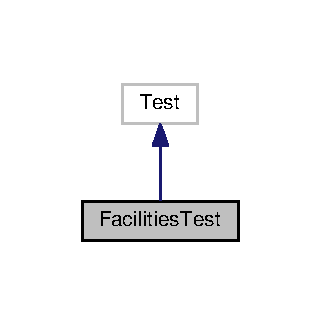
\includegraphics[width=154pt]{classFacilitiesTest__inherit__graph}
\end{center}
\end{figure}


Collaboration diagram for Facilities\-Test\-:
\nopagebreak
\begin{figure}[H]
\begin{center}
\leavevmode
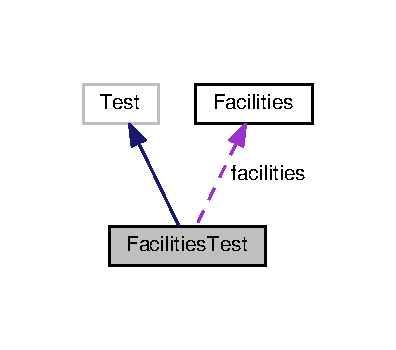
\includegraphics[width=190pt]{classFacilitiesTest__coll__graph}
\end{center}
\end{figure}
\subsection*{Public Attributes}
\begin{DoxyCompactItemize}
\item 
\hypertarget{classFacilitiesTest_afaf29496a8534f15a46465f571a2da26}{\hyperlink{classFacilities}{Facilities} {\bfseries facilities}}\label{classFacilitiesTest_afaf29496a8534f15a46465f571a2da26}

\end{DoxyCompactItemize}


The documentation for this class was generated from the following file\-:\begin{DoxyCompactItemize}
\item 
/home/aleksander/\-C\-Lion\-Projects/\-Zpr/test/Facilities\-Test.\-cpp\end{DoxyCompactItemize}

\hypertarget{classGridGUI}{\section{Grid\-G\-U\-I Class Reference}
\label{classGridGUI}\index{Grid\-G\-U\-I@{Grid\-G\-U\-I}}
}


The \hyperlink{classGridGUI}{Grid\-G\-U\-I} class.  




{\ttfamily \#include $<$gridgui.\-h$>$}



Inheritance diagram for Grid\-G\-U\-I\-:
\nopagebreak
\begin{figure}[H]
\begin{center}
\leavevmode
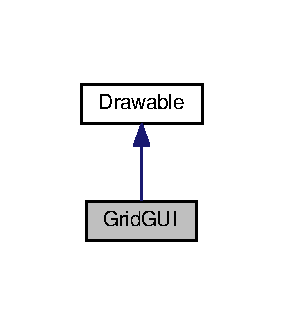
\includegraphics[width=136pt]{classGridGUI__inherit__graph}
\end{center}
\end{figure}


Collaboration diagram for Grid\-G\-U\-I\-:
\nopagebreak
\begin{figure}[H]
\begin{center}
\leavevmode
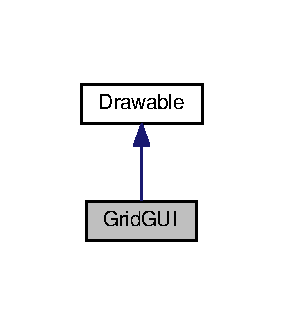
\includegraphics[width=136pt]{classGridGUI__coll__graph}
\end{center}
\end{figure}
\subsection*{Public Member Functions}
\begin{DoxyCompactItemize}
\item 
\hyperlink{classGridGUI_a26a49d8e03b995f94d4ba2f962447755}{Grid\-G\-U\-I} (unsigned int width, unsigned int height)
\begin{DoxyCompactList}\small\item\em \hyperlink{classGridGUI_a26a49d8e03b995f94d4ba2f962447755}{Grid\-G\-U\-I\-::\-Grid\-G\-U\-I}. \end{DoxyCompactList}\item 
void \hyperlink{classGridGUI_a733eb9089f663b943a4df35bd0deb0e9}{draw} (Q\-Painter \&painter) const override
\begin{DoxyCompactList}\small\item\em \hyperlink{classGridGUI_a733eb9089f663b943a4df35bd0deb0e9}{Grid\-G\-U\-I\-::draw}. \end{DoxyCompactList}\item 
\hypertarget{classGridGUI_a5a766544081b2b32622599271b8fdac3}{void {\bfseries set\-To} (unsigned int x, unsigned int y) override}\label{classGridGUI_a5a766544081b2b32622599271b8fdac3}

\item 
\hypertarget{classGridGUI_ad39aea9c016151e90c8809878a89ed0d}{bool {\bfseries intersects} (Q\-Rect \&rectangle) const override}\label{classGridGUI_ad39aea9c016151e90c8809878a89ed0d}

\end{DoxyCompactItemize}
\subsection*{Static Public Attributes}
\begin{DoxyCompactItemize}
\item 
static const Q\-Pen \hyperlink{classGridGUI_a0bdab0ceaf6c0009b26b344bb20e75a4}{P\-E\-N}
\item 
\hypertarget{classGridGUI_ae526a7b1f11279b5ec1515eb4e19c250}{static const int {\bfseries S\-I\-Z\-E} = 32}\label{classGridGUI_ae526a7b1f11279b5ec1515eb4e19c250}

\end{DoxyCompactItemize}


\subsection{Detailed Description}
The \hyperlink{classGridGUI}{Grid\-G\-U\-I} class. 

Class represents grid drawn on the screen. most of objects are snapped to this grid. It implements all necessary functions to be drawn. It also contains all variables thet define look of the grid. \begin{DoxyAuthor}{Author}
Pawel Rybak 
\end{DoxyAuthor}


\subsection{Constructor \& Destructor Documentation}
\hypertarget{classGridGUI_a26a49d8e03b995f94d4ba2f962447755}{\index{Grid\-G\-U\-I@{Grid\-G\-U\-I}!Grid\-G\-U\-I@{Grid\-G\-U\-I}}
\index{Grid\-G\-U\-I@{Grid\-G\-U\-I}!GridGUI@{Grid\-G\-U\-I}}
\subsubsection[{Grid\-G\-U\-I}]{\setlength{\rightskip}{0pt plus 5cm}Grid\-G\-U\-I\-::\-Grid\-G\-U\-I (
\begin{DoxyParamCaption}
\item[{unsigned int}]{width, }
\item[{unsigned int}]{height}
\end{DoxyParamCaption}
)}}\label{classGridGUI_a26a49d8e03b995f94d4ba2f962447755}


\hyperlink{classGridGUI_a26a49d8e03b995f94d4ba2f962447755}{Grid\-G\-U\-I\-::\-Grid\-G\-U\-I}. 


\begin{DoxyParams}{Parameters}
{\em width} & -\/ Width of the grid. \\
\hline
{\em height} & -\/ Height of the grid.\\
\hline
\end{DoxyParams}
Creates grid with given size. 

\subsection{Member Function Documentation}
\hypertarget{classGridGUI_a733eb9089f663b943a4df35bd0deb0e9}{\index{Grid\-G\-U\-I@{Grid\-G\-U\-I}!draw@{draw}}
\index{draw@{draw}!GridGUI@{Grid\-G\-U\-I}}
\subsubsection[{draw}]{\setlength{\rightskip}{0pt plus 5cm}void Grid\-G\-U\-I\-::draw (
\begin{DoxyParamCaption}
\item[{Q\-Painter \&}]{painter}
\end{DoxyParamCaption}
) const\hspace{0.3cm}{\ttfamily [override]}, {\ttfamily [virtual]}}}\label{classGridGUI_a733eb9089f663b943a4df35bd0deb0e9}


\hyperlink{classGridGUI_a733eb9089f663b943a4df35bd0deb0e9}{Grid\-G\-U\-I\-::draw}. 


\begin{DoxyParams}{Parameters}
{\em painter} & -\/ Reference to painter object.\\
\hline
\end{DoxyParams}
Function draws lines using painter given as argument. Lines, both vertical and horizontal, starts at 0, and are drawn with equal spacing until next line would be further than size of grid. 

Implements \hyperlink{classDrawable}{Drawable}.



\subsection{Member Data Documentation}
\hypertarget{classGridGUI_a0bdab0ceaf6c0009b26b344bb20e75a4}{\index{Grid\-G\-U\-I@{Grid\-G\-U\-I}!P\-E\-N@{P\-E\-N}}
\index{P\-E\-N@{P\-E\-N}!GridGUI@{Grid\-G\-U\-I}}
\subsubsection[{P\-E\-N}]{\setlength{\rightskip}{0pt plus 5cm}const Q\-Pen Grid\-G\-U\-I\-::\-P\-E\-N\hspace{0.3cm}{\ttfamily [static]}}}\label{classGridGUI_a0bdab0ceaf6c0009b26b344bb20e75a4}
P\-R\-O\-P\-E\-R\-T\-I\-E\-S

I\-N\-I\-T\-I\-A\-L\-I\-Z\-E P\-R\-O\-P\-E\-R\-T\-I\-E\-S 

The documentation for this class was generated from the following files\-:\begin{DoxyCompactItemize}
\item 
/home/aleksander/\-C\-Lion\-Projects/\-Zpr/src/\-G\-U\-I/gridgui.\-h\item 
/home/aleksander/\-C\-Lion\-Projects/\-Zpr/src/\-G\-U\-I/gridgui.\-cpp\end{DoxyCompactItemize}

\hypertarget{classHuman}{\section{Human Class Reference}
\label{classHuman}\index{Human@{Human}}
}


{\ttfamily \#include $<$Movable.\-h$>$}



Inheritance diagram for Human\-:
\nopagebreak
\begin{figure}[H]
\begin{center}
\leavevmode
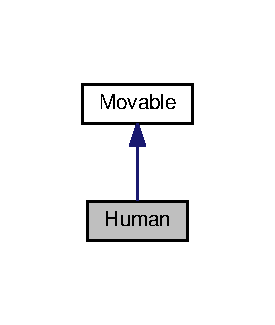
\includegraphics[width=132pt]{classHuman__inherit__graph}
\end{center}
\end{figure}


Collaboration diagram for Human\-:
\nopagebreak
\begin{figure}[H]
\begin{center}
\leavevmode
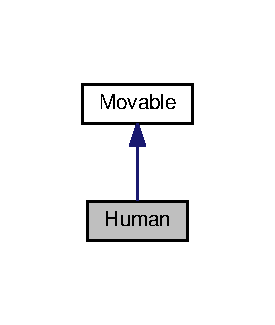
\includegraphics[width=132pt]{classHuman__coll__graph}
\end{center}
\end{figure}
\subsection*{Static Public Member Functions}
\begin{DoxyCompactItemize}
\item 
static Ptr\-Human \hyperlink{classHuman_a09310c96463d7b8f25d49fdee36482ec}{create\-Human} (const \hyperlink{classPoint}{Point} \&start\-Point, const std\-::vector$<$ Ptr\-To\-Const\-Point $>$ \&points, const int speed, const unsigned int id)
\end{DoxyCompactItemize}
\subsection*{Additional Inherited Members}


\subsection{Detailed Description}
Represents human. \begin{DoxyAuthor}{Author}
Aleksander Brzozowski 
\end{DoxyAuthor}


\subsection{Member Function Documentation}
\hypertarget{classHuman_a09310c96463d7b8f25d49fdee36482ec}{\index{Human@{Human}!create\-Human@{create\-Human}}
\index{create\-Human@{create\-Human}!Human@{Human}}
\subsubsection[{create\-Human}]{\setlength{\rightskip}{0pt plus 5cm}Ptr\-Human Human\-::create\-Human (
\begin{DoxyParamCaption}
\item[{const {\bf Point} \&}]{start\-Point, }
\item[{const std\-::vector$<$ Ptr\-To\-Const\-Point $>$ \&}]{points, }
\item[{const int}]{speed, }
\item[{const unsigned int}]{id}
\end{DoxyParamCaption}
)\hspace{0.3cm}{\ttfamily [static]}}}\label{classHuman_a09310c96463d7b8f25d49fdee36482ec}
Constructs \hyperlink{classHuman}{Human}. 
\begin{DoxyParams}{Parameters}
{\em start\-Point} & \hyperlink{classPoint}{Point} in which human will start \\
\hline
{\em points} & Points to follow by human \\
\hline
{\em speed} & \hyperlink{classHuman}{Human}'s speed \\
\hline
{\em id} & \hyperlink{classHuman}{Human}'s id \\
\hline
\end{DoxyParams}
\begin{DoxyReturn}{Returns}
Created human 
\end{DoxyReturn}


The documentation for this class was generated from the following files\-:\begin{DoxyCompactItemize}
\item 
/home/aleksander/\-C\-Lion\-Projects/\-Zpr/src/Movable.\-h\item 
/home/aleksander/\-C\-Lion\-Projects/\-Zpr/src/Movable.\-cpp\end{DoxyCompactItemize}

\hypertarget{classHumanRoute}{\section{Human\-Route Class Reference}
\label{classHumanRoute}\index{Human\-Route@{Human\-Route}}
}


{\ttfamily \#include $<$Human\-Route.\-h$>$}



Inheritance diagram for Human\-Route\-:
\nopagebreak
\begin{figure}[H]
\begin{center}
\leavevmode
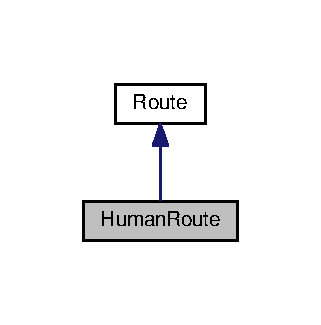
\includegraphics[width=154pt]{classHumanRoute__inherit__graph}
\end{center}
\end{figure}


Collaboration diagram for Human\-Route\-:
\nopagebreak
\begin{figure}[H]
\begin{center}
\leavevmode
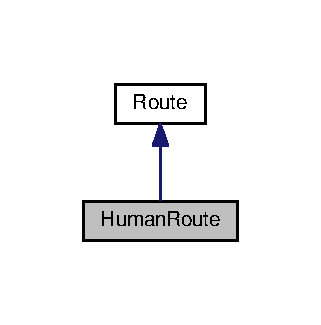
\includegraphics[width=154pt]{classHumanRoute__coll__graph}
\end{center}
\end{figure}
\subsection*{Public Member Functions}
\begin{DoxyCompactItemize}
\item 
\hyperlink{classHumanRoute_a2bbf33e39be296250ae7fcf55b7cfedf}{Human\-Route} (const std\-::vector$<$ Ptr\-To\-Const\-Point $>$ \&points)
\item 
bool \hyperlink{classHumanRoute_a89c5021044b130a2928eb933111bf390}{next\-Point} () override
\item 
bool \hyperlink{classHumanRoute_aee549e955710a5217ba763d2320fb0ea}{is\-End} () override
\end{DoxyCompactItemize}


\subsection{Detailed Description}
Represents route for \hyperlink{classHuman}{Human}. \begin{DoxyAuthor}{Author}
Aleksander Brzozowski 
\end{DoxyAuthor}


\subsection{Constructor \& Destructor Documentation}
\hypertarget{classHumanRoute_a2bbf33e39be296250ae7fcf55b7cfedf}{\index{Human\-Route@{Human\-Route}!Human\-Route@{Human\-Route}}
\index{Human\-Route@{Human\-Route}!HumanRoute@{Human\-Route}}
\subsubsection[{Human\-Route}]{\setlength{\rightskip}{0pt plus 5cm}Human\-Route\-::\-Human\-Route (
\begin{DoxyParamCaption}
\item[{const std\-::vector$<$ Ptr\-To\-Const\-Point $>$ \&}]{points}
\end{DoxyParamCaption}
)}}\label{classHumanRoute_a2bbf33e39be296250ae7fcf55b7cfedf}
Constructs \hyperlink{classHumanRoute}{Human\-Route}. 
\begin{DoxyParams}{Parameters}
{\em points} & Points to fallow by route. \\
\hline
\end{DoxyParams}


\subsection{Member Function Documentation}
\hypertarget{classHumanRoute_aee549e955710a5217ba763d2320fb0ea}{\index{Human\-Route@{Human\-Route}!is\-End@{is\-End}}
\index{is\-End@{is\-End}!HumanRoute@{Human\-Route}}
\subsubsection[{is\-End}]{\setlength{\rightskip}{0pt plus 5cm}bool Human\-Route\-::is\-End (
\begin{DoxyParamCaption}
{}
\end{DoxyParamCaption}
)\hspace{0.3cm}{\ttfamily [override]}, {\ttfamily [virtual]}}}\label{classHumanRoute_aee549e955710a5217ba763d2320fb0ea}
Checks is it end of \hyperlink{classRoute}{Route}. \begin{DoxyReturn}{Returns}
is end of \hyperlink{classRoute}{Route} 
\end{DoxyReturn}


Implements \hyperlink{classRoute_a0e1d104b56c768549f1b4fe4b575a6f5}{Route}.

\hypertarget{classHumanRoute_a89c5021044b130a2928eb933111bf390}{\index{Human\-Route@{Human\-Route}!next\-Point@{next\-Point}}
\index{next\-Point@{next\-Point}!HumanRoute@{Human\-Route}}
\subsubsection[{next\-Point}]{\setlength{\rightskip}{0pt plus 5cm}bool Human\-Route\-::next\-Point (
\begin{DoxyParamCaption}
{}
\end{DoxyParamCaption}
)\hspace{0.3cm}{\ttfamily [override]}, {\ttfamily [virtual]}}}\label{classHumanRoute_a89c5021044b130a2928eb933111bf390}
Switches to the next point of route. \begin{DoxyReturn}{Returns}
Is next point of route 
\end{DoxyReturn}


Implements \hyperlink{classRoute_a27bb16170420801b5c191e9aea0134f1}{Route}.



The documentation for this class was generated from the following files\-:\begin{DoxyCompactItemize}
\item 
/home/aleksander/\-C\-Lion\-Projects/\-Zpr/src/Human\-Route.\-h\item 
/home/aleksander/\-C\-Lion\-Projects/\-Zpr/src/Human\-Route.\-cpp\end{DoxyCompactItemize}

\hypertarget{classLineSegment}{\section{Line\-Segment Class Reference}
\label{classLineSegment}\index{Line\-Segment@{Line\-Segment}}
}


{\ttfamily \#include $<$Line\-Segment.\-h$>$}

\subsection*{Public Member Functions}
\begin{DoxyCompactItemize}
\item 
\hyperlink{classLineSegment_aedf097c6e1e883c4afa3b73f506ec14a}{Line\-Segment} (const \hyperlink{classPoint}{Point} \&point\-A, const \hyperlink{classPoint}{Point} \&point\-B)
\item 
std\-::pair$<$ float, float $>$ \hyperlink{classLineSegment_a925e2e233b920ca5ddc28e6e069217d1}{intersection\-Point} (const \hyperlink{classLineSegment}{Line\-Segment} \&line\-Segment) const 
\item 
bool \hyperlink{classLineSegment_ac7c1a4f6079ce306b855d5d438abbcb7}{has\-Intersection} (const \hyperlink{classLineSegment}{Line\-Segment} \&line\-Segment) const 
\end{DoxyCompactItemize}


\subsection{Detailed Description}
Represents segment line. Stores straight line equation\-: (y -\/ ya) $\ast$ (xb -\/ xa) -\/ (yb -\/ ya) $\ast$ (x -\/ xa) = 0 y $\ast$ (xb -\/ xa) -\/ x $\ast$ (yb -\/ ya) = ya $\ast$ (xb -\/ xa) -\/ xa $\ast$ (yb -\/ ya) and limits of segment line (x and y limits) \begin{DoxyAuthor}{Author}
Aleksander Brzozowski 
\end{DoxyAuthor}


\subsection{Constructor \& Destructor Documentation}
\hypertarget{classLineSegment_aedf097c6e1e883c4afa3b73f506ec14a}{\index{Line\-Segment@{Line\-Segment}!Line\-Segment@{Line\-Segment}}
\index{Line\-Segment@{Line\-Segment}!LineSegment@{Line\-Segment}}
\subsubsection[{Line\-Segment}]{\setlength{\rightskip}{0pt plus 5cm}Line\-Segment\-::\-Line\-Segment (
\begin{DoxyParamCaption}
\item[{const {\bf Point} \&}]{point\-A, }
\item[{const {\bf Point} \&}]{point\-B}
\end{DoxyParamCaption}
)}}\label{classLineSegment_aedf097c6e1e883c4afa3b73f506ec14a}
Constructs \hyperlink{classLineSegment}{Line\-Segment}. 
\begin{DoxyExceptions}{Exceptions}
{\em std\-::invalid\-\_\-argument} & when points are same \\
\hline
\end{DoxyExceptions}

\begin{DoxyParams}{Parameters}
{\em point\-A} & First point of line segment \\
\hline
{\em point\-B} & Second point of line segment \\
\hline
\end{DoxyParams}


\subsection{Member Function Documentation}
\hypertarget{classLineSegment_ac7c1a4f6079ce306b855d5d438abbcb7}{\index{Line\-Segment@{Line\-Segment}!has\-Intersection@{has\-Intersection}}
\index{has\-Intersection@{has\-Intersection}!LineSegment@{Line\-Segment}}
\subsubsection[{has\-Intersection}]{\setlength{\rightskip}{0pt plus 5cm}bool Line\-Segment\-::has\-Intersection (
\begin{DoxyParamCaption}
\item[{const {\bf Line\-Segment} \&}]{line\-Segment}
\end{DoxyParamCaption}
) const}}\label{classLineSegment_ac7c1a4f6079ce306b855d5d438abbcb7}
Checks whether line segments have intersection point. 
\begin{DoxyParams}{Parameters}
{\em line\-Segment} & Line segment to check \\
\hline
\end{DoxyParams}
\begin{DoxyReturn}{Returns}
Has line segments intersection point 
\end{DoxyReturn}
\hypertarget{classLineSegment_a925e2e233b920ca5ddc28e6e069217d1}{\index{Line\-Segment@{Line\-Segment}!intersection\-Point@{intersection\-Point}}
\index{intersection\-Point@{intersection\-Point}!LineSegment@{Line\-Segment}}
\subsubsection[{intersection\-Point}]{\setlength{\rightskip}{0pt plus 5cm}std\-::pair$<$ float, float $>$ Line\-Segment\-::intersection\-Point (
\begin{DoxyParamCaption}
\item[{const {\bf Line\-Segment} \&}]{line\-Segment}
\end{DoxyParamCaption}
) const}}\label{classLineSegment_a925e2e233b920ca5ddc28e6e069217d1}
Computes intersection point of line segments. 
\begin{DoxyExceptions}{Exceptions}
{\em std\-::invalid\-\_\-argument} & when there isn't intersection point \\
\hline
\end{DoxyExceptions}

\begin{DoxyParams}{Parameters}
{\em line\-Segment} & Line segment used to compute intersection point \\
\hline
\end{DoxyParams}
\begin{DoxyReturn}{Returns}
Intersection point as a pair of x and y (first x, second y) 
\end{DoxyReturn}


The documentation for this class was generated from the following files\-:\begin{DoxyCompactItemize}
\item 
/home/aleksander/\-C\-Lion\-Projects/\-Zpr/src/Line\-Segment.\-h\item 
/home/aleksander/\-C\-Lion\-Projects/\-Zpr/src/Line\-Segment.\-cpp\end{DoxyCompactItemize}

\hypertarget{classMainWindow}{\section{Main\-Window Class Reference}
\label{classMainWindow}\index{Main\-Window@{Main\-Window}}
}


The \hyperlink{classMainWindow}{Main\-Window} class.  




{\ttfamily \#include $<$mainwindow.\-h$>$}



Inheritance diagram for Main\-Window\-:
\nopagebreak
\begin{figure}[H]
\begin{center}
\leavevmode
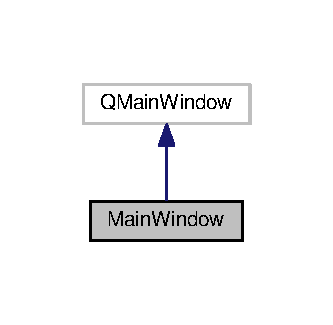
\includegraphics[width=160pt]{classMainWindow__inherit__graph}
\end{center}
\end{figure}


Collaboration diagram for Main\-Window\-:
\nopagebreak
\begin{figure}[H]
\begin{center}
\leavevmode
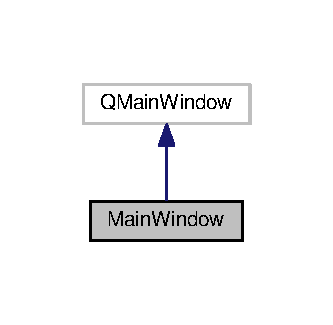
\includegraphics[width=160pt]{classMainWindow__coll__graph}
\end{center}
\end{figure}
\subsection*{Public Member Functions}
\begin{DoxyCompactItemize}
\item 
void \hyperlink{classMainWindow_a9907ff1d21c9e2cc7078a2b5ba043b52}{set\-Map} (std\-::shared\-\_\-ptr$<$ \hyperlink{classMap}{Map} $>$ map)
\begin{DoxyCompactList}\small\item\em \hyperlink{classMainWindow_a9907ff1d21c9e2cc7078a2b5ba043b52}{Main\-Window\-::set\-Map}. \end{DoxyCompactList}\item 
void \hyperlink{classMainWindow_a8a2dbcb697f105c012e3ca3704d95b77}{set\-Car} (const unsigned int id, const unsigned int x, const unsigned int y, const bool fast=false)
\begin{DoxyCompactList}\small\item\em \hyperlink{classMainWindow_a8a2dbcb697f105c012e3ca3704d95b77}{Main\-Window\-::set\-Car}. \end{DoxyCompactList}\item 
void \hyperlink{classMainWindow_a41c3fa9c4208016244cfc988ec0967ca}{set\-Ppl} (const unsigned int id, const unsigned int x, const unsigned int y)
\begin{DoxyCompactList}\small\item\em \hyperlink{classMainWindow_a41c3fa9c4208016244cfc988ec0967ca}{Main\-Window\-::set\-Ppl}. \end{DoxyCompactList}\item 
void \hyperlink{classMainWindow_a3ec289e870edc7413a1e03245eee4e1a}{remove\-Object} (const unsigned int id)
\begin{DoxyCompactList}\small\item\em \hyperlink{classMainWindow_a3ec289e870edc7413a1e03245eee4e1a}{Main\-Window\-::remove\-Object}. \end{DoxyCompactList}\item 
void \hyperlink{classMainWindow_ab27297114529e4c16d6d8d7a54927a0e}{refresh} ()
\begin{DoxyCompactList}\small\item\em \hyperlink{classMainWindow_ab27297114529e4c16d6d8d7a54927a0e}{Main\-Window\-::refresh}. \end{DoxyCompactList}\item 
void \hyperlink{classMainWindow_a5912f1655918f9f941280fc900695594}{reset\-Label} ()
\begin{DoxyCompactList}\small\item\em \hyperlink{classMainWindow_a5912f1655918f9f941280fc900695594}{Main\-Window\-::reset\-Label}. \end{DoxyCompactList}\end{DoxyCompactItemize}
\subsection*{Static Public Member Functions}
\begin{DoxyCompactItemize}
\item 
static \hyperlink{classMainWindow}{Main\-Window} \& \hyperlink{classMainWindow_a17b66394011720014a82ed3457a48bd3}{get\-Instance} ()
\begin{DoxyCompactList}\small\item\em \hyperlink{classMainWindow_a17b66394011720014a82ed3457a48bd3}{Main\-Window\-::get\-Instance}. \end{DoxyCompactList}\end{DoxyCompactItemize}
\subsection*{Static Public Attributes}
\begin{DoxyCompactItemize}
\item 
\hypertarget{classMainWindow_ac52c27e88f64214983e13638b1c73e80}{static const \\*
std\-::chrono\-::milliseconds \hyperlink{classMainWindow_ac52c27e88f64214983e13638b1c73e80}{R\-E\-F\-R\-E\-S\-H\-\_\-\-T\-I\-M\-E} = std\-::chrono\-::milliseconds(50)}\label{classMainWindow_ac52c27e88f64214983e13638b1c73e80}

\begin{DoxyCompactList}\small\item\em \hyperlink{classMainWindow_ac52c27e88f64214983e13638b1c73e80}{Main\-Window\-::\-R\-E\-F\-R\-E\-S\-H\-\_\-\-T\-I\-M\-E}. Time between cars movement. \end{DoxyCompactList}\item 
\hypertarget{classMainWindow_a1e3a4f8c96328a2f84b8382649d04967}{static const std\-::chrono\-::seconds \hyperlink{classMainWindow_a1e3a4f8c96328a2f84b8382649d04967}{C\-A\-M\-E\-R\-A\-\_\-\-S\-C\-A\-N\-\_\-\-F\-R\-E\-Q} = std\-::chrono\-::seconds(1)}\label{classMainWindow_a1e3a4f8c96328a2f84b8382649d04967}

\begin{DoxyCompactList}\small\item\em \hyperlink{classMainWindow_a1e3a4f8c96328a2f84b8382649d04967}{Main\-Window\-::\-C\-A\-M\-E\-R\-A\-\_\-\-S\-C\-A\-N\-\_\-\-F\-R\-E\-Q}. Time between camera scans. \end{DoxyCompactList}\end{DoxyCompactItemize}


\subsection{Detailed Description}
The \hyperlink{classMainWindow}{Main\-Window} class. 

Class is a facade for G\-U\-I part of project. It provides methods to set objects to pointed position, remove them and refresh the rendered area. Class is singleton, so only way to access it is through appropriate method. 

\subsection{Member Function Documentation}
\hypertarget{classMainWindow_a17b66394011720014a82ed3457a48bd3}{\index{Main\-Window@{Main\-Window}!get\-Instance@{get\-Instance}}
\index{get\-Instance@{get\-Instance}!MainWindow@{Main\-Window}}
\subsubsection[{get\-Instance}]{\setlength{\rightskip}{0pt plus 5cm}{\bf Main\-Window} \& Main\-Window\-::get\-Instance (
\begin{DoxyParamCaption}
{}
\end{DoxyParamCaption}
)\hspace{0.3cm}{\ttfamily [static]}}}\label{classMainWindow_a17b66394011720014a82ed3457a48bd3}


\hyperlink{classMainWindow_a17b66394011720014a82ed3457a48bd3}{Main\-Window\-::get\-Instance}. 

\begin{DoxyReturn}{Returns}
Returns instance of \hyperlink{classMainWindow}{Main\-Window} object. Only way to create that object. 
\end{DoxyReturn}
\hypertarget{classMainWindow_ab27297114529e4c16d6d8d7a54927a0e}{\index{Main\-Window@{Main\-Window}!refresh@{refresh}}
\index{refresh@{refresh}!MainWindow@{Main\-Window}}
\subsubsection[{refresh}]{\setlength{\rightskip}{0pt plus 5cm}void Main\-Window\-::refresh (
\begin{DoxyParamCaption}
{}
\end{DoxyParamCaption}
)}}\label{classMainWindow_ab27297114529e4c16d6d8d7a54927a0e}


\hyperlink{classMainWindow_ab27297114529e4c16d6d8d7a54927a0e}{Main\-Window\-::refresh}. 

Refreshes rendered area. Render area doesn't refresh itself, so it can be done only when needed. \hypertarget{classMainWindow_a3ec289e870edc7413a1e03245eee4e1a}{\index{Main\-Window@{Main\-Window}!remove\-Object@{remove\-Object}}
\index{remove\-Object@{remove\-Object}!MainWindow@{Main\-Window}}
\subsubsection[{remove\-Object}]{\setlength{\rightskip}{0pt plus 5cm}void Main\-Window\-::remove\-Object (
\begin{DoxyParamCaption}
\item[{const unsigned int}]{id}
\end{DoxyParamCaption}
)}}\label{classMainWindow_a3ec289e870edc7413a1e03245eee4e1a}


\hyperlink{classMainWindow_a3ec289e870edc7413a1e03245eee4e1a}{Main\-Window\-::remove\-Object}. 


\begin{DoxyParams}{Parameters}
{\em id} & -\/ object I\-D.\\
\hline
\end{DoxyParams}
Removes object from list of object that are being redrawn. Supposed to be called when object doesn't exist anymore. \hypertarget{classMainWindow_a5912f1655918f9f941280fc900695594}{\index{Main\-Window@{Main\-Window}!reset\-Label@{reset\-Label}}
\index{reset\-Label@{reset\-Label}!MainWindow@{Main\-Window}}
\subsubsection[{reset\-Label}]{\setlength{\rightskip}{0pt plus 5cm}void Main\-Window\-::reset\-Label (
\begin{DoxyParamCaption}
{}
\end{DoxyParamCaption}
)}}\label{classMainWindow_a5912f1655918f9f941280fc900695594}


\hyperlink{classMainWindow_a5912f1655918f9f941280fc900695594}{Main\-Window\-::reset\-Label}. 

Sets status label to say that no option is chosen and advise to choose one. \hypertarget{classMainWindow_a8a2dbcb697f105c012e3ca3704d95b77}{\index{Main\-Window@{Main\-Window}!set\-Car@{set\-Car}}
\index{set\-Car@{set\-Car}!MainWindow@{Main\-Window}}
\subsubsection[{set\-Car}]{\setlength{\rightskip}{0pt plus 5cm}void Main\-Window\-::set\-Car (
\begin{DoxyParamCaption}
\item[{const unsigned int}]{id, }
\item[{const unsigned int}]{x, }
\item[{const unsigned int}]{y, }
\item[{const bool}]{fast = {\ttfamily false}}
\end{DoxyParamCaption}
)}}\label{classMainWindow_a8a2dbcb697f105c012e3ca3704d95b77}


\hyperlink{classMainWindow_a8a2dbcb697f105c012e3ca3704d95b77}{Main\-Window\-::set\-Car}. 


\begin{DoxyParams}{Parameters}
{\em id} & -\/ car I\-D. \\
\hline
{\em x} & -\/ position X. \\
\hline
{\em y} & -\/ position Y. \\
\hline
{\em fast} & -\/ flag says if car is fast car or not. false by default.\\
\hline
\end{DoxyParams}
Sets car to appropriate position, and specify type of car being set. \hypertarget{classMainWindow_a9907ff1d21c9e2cc7078a2b5ba043b52}{\index{Main\-Window@{Main\-Window}!set\-Map@{set\-Map}}
\index{set\-Map@{set\-Map}!MainWindow@{Main\-Window}}
\subsubsection[{set\-Map}]{\setlength{\rightskip}{0pt plus 5cm}void Main\-Window\-::set\-Map (
\begin{DoxyParamCaption}
\item[{std\-::shared\-\_\-ptr$<$ {\bf Map} $>$}]{map}
\end{DoxyParamCaption}
)}}\label{classMainWindow_a9907ff1d21c9e2cc7078a2b5ba043b52}


\hyperlink{classMainWindow_a9907ff1d21c9e2cc7078a2b5ba043b52}{Main\-Window\-::set\-Map}. 


\begin{DoxyParams}{Parameters}
{\em map} & \\
\hline
\end{DoxyParams}
Sets map object to allow pass user-\/generated events to model. Without map any user input won't take any affect. \begin{DoxySeeAlso}{See Also}
\hyperlink{classEventInterpreter_a6ca1d621b8ef0297675be928b996ae8b}{Event\-Interpreter\-::set\-Map}. 
\end{DoxySeeAlso}
\hypertarget{classMainWindow_a41c3fa9c4208016244cfc988ec0967ca}{\index{Main\-Window@{Main\-Window}!set\-Ppl@{set\-Ppl}}
\index{set\-Ppl@{set\-Ppl}!MainWindow@{Main\-Window}}
\subsubsection[{set\-Ppl}]{\setlength{\rightskip}{0pt plus 5cm}void Main\-Window\-::set\-Ppl (
\begin{DoxyParamCaption}
\item[{const unsigned int}]{id, }
\item[{const unsigned int}]{x, }
\item[{const unsigned int}]{y}
\end{DoxyParamCaption}
)}}\label{classMainWindow_a41c3fa9c4208016244cfc988ec0967ca}


\hyperlink{classMainWindow_a41c3fa9c4208016244cfc988ec0967ca}{Main\-Window\-::set\-Ppl}. 


\begin{DoxyParams}{Parameters}
{\em id} & -\/ person I\-D. \\
\hline
{\em x} & -\/ position X. \\
\hline
{\em y} & -\/ position Y.\\
\hline
\end{DoxyParams}
Sets person to appropriate position, so it can be repainted where it actually is. 

The documentation for this class was generated from the following files\-:\begin{DoxyCompactItemize}
\item 
/home/aleksander/\-C\-Lion\-Projects/\-Zpr/src/\-G\-U\-I/mainwindow.\-h\item 
/home/aleksander/\-C\-Lion\-Projects/\-Zpr/src/\-G\-U\-I/mainwindow.\-cpp\end{DoxyCompactItemize}

\hypertarget{classUi_1_1MainWindow}{\section{Ui\-:\-:Main\-Window Class Reference}
\label{classUi_1_1MainWindow}\index{Ui\-::\-Main\-Window@{Ui\-::\-Main\-Window}}
}


Inheritance diagram for Ui\-:\-:Main\-Window\-:
\nopagebreak
\begin{figure}[H]
\begin{center}
\leavevmode
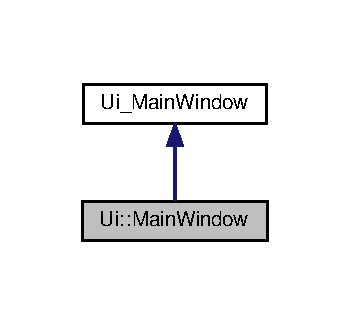
\includegraphics[width=168pt]{classUi_1_1MainWindow__inherit__graph}
\end{center}
\end{figure}


Collaboration diagram for Ui\-:\-:Main\-Window\-:
\nopagebreak
\begin{figure}[H]
\begin{center}
\leavevmode
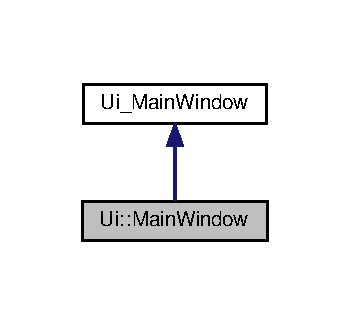
\includegraphics[width=168pt]{classUi_1_1MainWindow__coll__graph}
\end{center}
\end{figure}
\subsection*{Additional Inherited Members}


The documentation for this class was generated from the following file\-:\begin{DoxyCompactItemize}
\item 
/home/aleksander/\-C\-Lion\-Projects/\-Zpr/src/\-G\-U\-I/ui\-\_\-mainwindow.\-h\end{DoxyCompactItemize}

\hypertarget{classMap}{\section{Map Class Reference}
\label{classMap}\index{Map@{Map}}
}


Class allowing to create map and simulate traffics.  




{\ttfamily \#include $<$Map.\-h$>$}

\subsection*{Public Member Functions}
\begin{DoxyCompactItemize}
\item 
\hyperlink{classMap_a0f5ad0fd4563497b4214038cbca8b582}{Map} ()
\item 
bool \hyperlink{classMap_a9e4f8c8c213327b8b82f22280a11bd97}{create\-Road} (Ptr\-To\-Const\-Point, Ptr\-To\-Const\-Point)
\begin{DoxyCompactList}\small\item\em Creating new road and crosses from starting to ending point. \end{DoxyCompactList}\item 
void \hyperlink{classMap_a84db9fe1c1159747bc76790e1a839d7e}{create\-Car} (Ptr\-To\-Const\-Point, Ptr\-To\-Const\-Point, int)
\begin{DoxyCompactList}\small\item\em Calls creating methods in object of \hyperlink{classMovableFactory}{Movable\-Factory} type. \end{DoxyCompactList}\item 
void \hyperlink{classMap_a1a7df4e0e2269ed6d0594217c268ecc5}{create\-Human} (Ptr\-To\-Const\-Point, Ptr\-To\-Const\-Point, int)
\begin{DoxyCompactList}\small\item\em Calls creating methods in object of \hyperlink{classMovableFactory}{Movable\-Factory} type. \end{DoxyCompactList}\item 
bool \hyperlink{classMap_a691b0f6188a75243bf9201716ec65dd8}{create\-Building} (const \hyperlink{classPoint}{Point} \&upper\-Left, const \hyperlink{classPoint}{Point} \&lower\-Right)
\item 
void \hyperlink{classMap_a30ca1fc5c2c5dca2d75f936ebcd0f069}{create\-Camera} (const \hyperlink{classPoint}{Point} \&start\-Point, const \hyperlink{classPoint}{Point} \&end\-Point, double angle)
\item 
void \hyperlink{classMap_afb929e0412a0a74f94221a6476647eaa}{set\-Running\-Movable\-Permission} (bool)
\begin{DoxyCompactList}\small\item\em Running new thread for movables. \end{DoxyCompactList}\item 
void \hyperlink{classMap_a2cfa2043b101dfa956436a905794d9b5}{set\-Camera\-Scanning\-Permission} (bool)
\begin{DoxyCompactList}\small\item\em Running new thread for cameras. \end{DoxyCompactList}\item 
void \hyperlink{classMap_add4f93b254f5527945ae627db3878bae}{run\-Running\-Movables} ()
\begin{DoxyCompactList}\small\item\em Main method for running movables thread. \end{DoxyCompactList}\item 
\hypertarget{classMap_af5aea906aea8e3497f8300f06802270a}{void \hyperlink{classMap_af5aea906aea8e3497f8300f06802270a}{run\-Cameras\-Scanning} ()}\label{classMap_af5aea906aea8e3497f8300f06802270a}

\begin{DoxyCompactList}\small\item\em Method runs cameras scanning in new thread. \end{DoxyCompactList}\end{DoxyCompactItemize}


\subsection{Detailed Description}
Class allowing to create map and simulate traffics. 

Contains crosses and movables factories allowing G\-U\-I eassily creating map and threads to run the simulation 

\subsection{Constructor \& Destructor Documentation}
\hypertarget{classMap_a0f5ad0fd4563497b4214038cbca8b582}{\index{Map@{Map}!Map@{Map}}
\index{Map@{Map}!Map@{Map}}
\subsubsection[{Map}]{\setlength{\rightskip}{0pt plus 5cm}Map\-::\-Map (
\begin{DoxyParamCaption}
{}
\end{DoxyParamCaption}
)}}\label{classMap_a0f5ad0fd4563497b4214038cbca8b582}
Empty constructor. 

\subsection{Member Function Documentation}
\hypertarget{classMap_a691b0f6188a75243bf9201716ec65dd8}{\index{Map@{Map}!create\-Building@{create\-Building}}
\index{create\-Building@{create\-Building}!Map@{Map}}
\subsubsection[{create\-Building}]{\setlength{\rightskip}{0pt plus 5cm}bool Map\-::create\-Building (
\begin{DoxyParamCaption}
\item[{const {\bf Point} \&}]{upper\-Left, }
\item[{const {\bf Point} \&}]{lower\-Right}
\end{DoxyParamCaption}
)}}\label{classMap_a691b0f6188a75243bf9201716ec65dd8}
Adds \hyperlink{classBuilding}{Building} represented by arguments of function. 
\begin{DoxyParams}{Parameters}
{\em upper\-Left} & \hyperlink{classPoint}{Point} in the upper left of building \\
\hline
{\em lower\-Right} & \hyperlink{classPoint}{Point} in the lower right of building \\
\hline
\end{DoxyParams}
\begin{DoxyReturn}{Returns}
Is building created 
\end{DoxyReturn}
\hypertarget{classMap_a30ca1fc5c2c5dca2d75f936ebcd0f069}{\index{Map@{Map}!create\-Camera@{create\-Camera}}
\index{create\-Camera@{create\-Camera}!Map@{Map}}
\subsubsection[{create\-Camera}]{\setlength{\rightskip}{0pt plus 5cm}void Map\-::create\-Camera (
\begin{DoxyParamCaption}
\item[{const {\bf Point} \&}]{start\-Point, }
\item[{const {\bf Point} \&}]{end\-Point, }
\item[{double}]{angle}
\end{DoxyParamCaption}
)}}\label{classMap_a30ca1fc5c2c5dca2d75f936ebcd0f069}
Adds \hyperlink{classCamera}{Camera} represented by arguments of function. 
\begin{DoxyParams}{Parameters}
{\em start\-Point} & \hyperlink{classCamera}{Camera}'s start point \\
\hline
{\em end\-Point} & \hyperlink{classCamera}{Camera}'s end point \\
\hline
{\em angle} & \hyperlink{classCamera}{Camera}'s angle \\
\hline
{\em accuracy} & \hyperlink{classCamera}{Camera}'s accuracy \\
\hline
\end{DoxyParams}
\hypertarget{classMap_a84db9fe1c1159747bc76790e1a839d7e}{\index{Map@{Map}!create\-Car@{create\-Car}}
\index{create\-Car@{create\-Car}!Map@{Map}}
\subsubsection[{create\-Car}]{\setlength{\rightskip}{0pt plus 5cm}void Map\-::create\-Car (
\begin{DoxyParamCaption}
\item[{Ptr\-To\-Const\-Point}]{starting\-Point, }
\item[{Ptr\-To\-Const\-Point}]{ending\-Point, }
\item[{int}]{speed}
\end{DoxyParamCaption}
)}}\label{classMap_a84db9fe1c1159747bc76790e1a839d7e}


Calls creating methods in object of \hyperlink{classMovableFactory}{Movable\-Factory} type. 


\begin{DoxyParams}{Parameters}
{\em starting\-Point} & as shared\-\_\-ptr to \hyperlink{classPoint}{Point}. \\
\hline
{\em ending\-Point} & as shared\-\_\-ptr to \hyperlink{classPoint}{Point}. \\
\hline
{\em speed} & as integer argument. \\
\hline
\end{DoxyParams}
\hypertarget{classMap_a1a7df4e0e2269ed6d0594217c268ecc5}{\index{Map@{Map}!create\-Human@{create\-Human}}
\index{create\-Human@{create\-Human}!Map@{Map}}
\subsubsection[{create\-Human}]{\setlength{\rightskip}{0pt plus 5cm}void Map\-::create\-Human (
\begin{DoxyParamCaption}
\item[{Ptr\-To\-Const\-Point}]{src, }
\item[{Ptr\-To\-Const\-Point}]{dst, }
\item[{int}]{speed}
\end{DoxyParamCaption}
)}}\label{classMap_a1a7df4e0e2269ed6d0594217c268ecc5}


Calls creating methods in object of \hyperlink{classMovableFactory}{Movable\-Factory} type. 


\begin{DoxyParams}{Parameters}
{\em src} & as shared\-\_\-ptr on \hyperlink{classPoint}{Point} type object, starting point. \\
\hline
{\em dst} & as shared\-\_\-ptr on \hyperlink{classPoint}{Point} type object, ending point. \\
\hline
{\em speed} & as integer argument, speed of human. \\
\hline
\end{DoxyParams}
\hypertarget{classMap_a9e4f8c8c213327b8b82f22280a11bd97}{\index{Map@{Map}!create\-Road@{create\-Road}}
\index{create\-Road@{create\-Road}!Map@{Map}}
\subsubsection[{create\-Road}]{\setlength{\rightskip}{0pt plus 5cm}bool Map\-::create\-Road (
\begin{DoxyParamCaption}
\item[{Ptr\-To\-Const\-Point}]{begin, }
\item[{Ptr\-To\-Const\-Point}]{end}
\end{DoxyParamCaption}
)}}\label{classMap_a9e4f8c8c213327b8b82f22280a11bd97}


Creating new road and crosses from starting to ending point. 

Checking if road may be created (for example checking if none of buildings is between these two points). If not -\/$>$ method returns false. In other case\-: calling crosses creating methods from object of \hyperlink{classCrossFactory}{Cross\-Factory} type. 
\begin{DoxyParams}{Parameters}
{\em begin} & as shared\-\_\-ptr to \hyperlink{classPoint}{Point}. \\
\hline
{\em end} & as shared\-\_\-ptr to \hyperlink{classPoint}{Point}. \\
\hline
\end{DoxyParams}
\begin{DoxyReturn}{Returns}
bool value. If true -\/$>$ new road was created. 
\end{DoxyReturn}
\hypertarget{classMap_add4f93b254f5527945ae627db3878bae}{\index{Map@{Map}!run\-Running\-Movables@{run\-Running\-Movables}}
\index{run\-Running\-Movables@{run\-Running\-Movables}!Map@{Map}}
\subsubsection[{run\-Running\-Movables}]{\setlength{\rightskip}{0pt plus 5cm}void Map\-::run\-Running\-Movables (
\begin{DoxyParamCaption}
{}
\end{DoxyParamCaption}
)}}\label{classMap_add4f93b254f5527945ae627db3878bae}


Main method for running movables thread. 

All of the movables are asked to make the next move. If movables end their journey, they are removed from the memory and G\-U\-I. At the end, thread falls asleep for the time set in G\-U\-I const values. \hypertarget{classMap_a2cfa2043b101dfa956436a905794d9b5}{\index{Map@{Map}!set\-Camera\-Scanning\-Permission@{set\-Camera\-Scanning\-Permission}}
\index{set\-Camera\-Scanning\-Permission@{set\-Camera\-Scanning\-Permission}!Map@{Map}}
\subsubsection[{set\-Camera\-Scanning\-Permission}]{\setlength{\rightskip}{0pt plus 5cm}void Map\-::set\-Camera\-Scanning\-Permission (
\begin{DoxyParamCaption}
\item[{bool}]{permission}
\end{DoxyParamCaption}
)}}\label{classMap_a2cfa2043b101dfa956436a905794d9b5}


Running new thread for cameras. 

If permission is true, new thread is created, where all of the movables run. If permission is false, the thread finishes. 
\begin{DoxyParams}{Parameters}
{\em permission} & says if running thread has to start or stop. \\
\hline
\end{DoxyParams}
\hypertarget{classMap_afb929e0412a0a74f94221a6476647eaa}{\index{Map@{Map}!set\-Running\-Movable\-Permission@{set\-Running\-Movable\-Permission}}
\index{set\-Running\-Movable\-Permission@{set\-Running\-Movable\-Permission}!Map@{Map}}
\subsubsection[{set\-Running\-Movable\-Permission}]{\setlength{\rightskip}{0pt plus 5cm}void Map\-::set\-Running\-Movable\-Permission (
\begin{DoxyParamCaption}
\item[{bool}]{permission}
\end{DoxyParamCaption}
)}}\label{classMap_afb929e0412a0a74f94221a6476647eaa}


Running new thread for movables. 

If permission is true, new thread is created, where all of the movables run. If permission is false, the thread finishes. 
\begin{DoxyParams}{Parameters}
{\em permission} & says if running thread has to start or to stop. \\
\hline
\end{DoxyParams}


The documentation for this class was generated from the following files\-:\begin{DoxyCompactItemize}
\item 
/home/aleksander/\-C\-Lion\-Projects/\-Zpr/src/\hyperlink{Map_8h}{Map.\-h}\item 
/home/aleksander/\-C\-Lion\-Projects/\-Zpr/src/\hyperlink{Map_8cpp}{Map.\-cpp}\end{DoxyCompactItemize}

\hypertarget{classMapArea}{\section{Map\-Area Class Reference}
\label{classMapArea}\index{Map\-Area@{Map\-Area}}
}


The \hyperlink{classMapArea}{Map\-Area} class. Object responsible for drawing objects on screen.  




{\ttfamily \#include $<$maparea.\-h$>$}



Inheritance diagram for Map\-Area\-:
\nopagebreak
\begin{figure}[H]
\begin{center}
\leavevmode
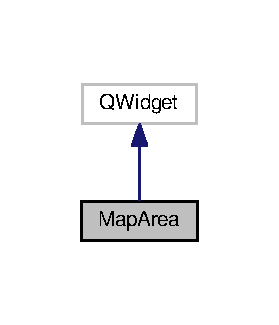
\includegraphics[width=134pt]{classMapArea__inherit__graph}
\end{center}
\end{figure}


Collaboration diagram for Map\-Area\-:
\nopagebreak
\begin{figure}[H]
\begin{center}
\leavevmode
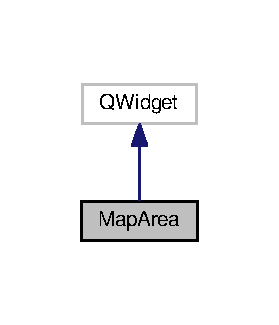
\includegraphics[width=134pt]{classMapArea__coll__graph}
\end{center}
\end{figure}
\subsection*{Public Slots}
\begin{DoxyCompactItemize}
\item 
\hypertarget{classMapArea_a1b2849d172c0941b3af68920dfd368de}{void \hyperlink{classMapArea_a1b2849d172c0941b3af68920dfd368de}{toggle\-Grid} ()}\label{classMapArea_a1b2849d172c0941b3af68920dfd368de}

\begin{DoxyCompactList}\small\item\em \hyperlink{classMapArea_a1b2849d172c0941b3af68920dfd368de}{Map\-Area\-::toggle\-Grid}. Toggles flag, whether grid is supposed to be drawn. After that map area is being redrawn. \end{DoxyCompactList}\item 
void \hyperlink{classMapArea_a71861f7055ae8107b8d69373c2629c5d}{register\-Road} (\hyperlink{classRoadGUI}{Road\-G\-U\-I} $\ast$)
\begin{DoxyCompactList}\small\item\em \hyperlink{classMapArea_a71861f7055ae8107b8d69373c2629c5d}{Map\-Area\-::register\-Road}. \end{DoxyCompactList}\item 
void \hyperlink{classMapArea_ace67fcedbc4d657eff057f0e67a22623}{register\-Drawable} (\hyperlink{classDrawable}{Drawable} $\ast$)
\begin{DoxyCompactList}\small\item\em \hyperlink{classMapArea_ace67fcedbc4d657eff057f0e67a22623}{Map\-Area\-::register\-Drawable}. \end{DoxyCompactList}\item 
void \hyperlink{classMapArea_ae50597953aea6204e9ab271dcf5b6154}{register\-Camera} (\hyperlink{classCameraGUI}{Camera\-G\-U\-I} $\ast$)
\begin{DoxyCompactList}\small\item\em \hyperlink{classMapArea_ae50597953aea6204e9ab271dcf5b6154}{Map\-Area\-::register\-Camera}. \end{DoxyCompactList}\end{DoxyCompactItemize}
\subsection*{Public Member Functions}
\begin{DoxyCompactItemize}
\item 
\hyperlink{classMapArea_aa1d27adefb4286cbb63b095e45fd0da1}{Map\-Area} (Q\-Widget $\ast$parent=0)
\begin{DoxyCompactList}\small\item\em \hyperlink{classMapArea_aa1d27adefb4286cbb63b095e45fd0da1}{Map\-Area\-::\-Map\-Area}. Constructor. Sets all variables. \end{DoxyCompactList}\item 
\hyperlink{classMapArea_a152c1aef862f93dd421b9026adf31e55}{$\sim$\-Map\-Area} ()
\begin{DoxyCompactList}\small\item\em \hyperlink{classMapArea_a152c1aef862f93dd421b9026adf31e55}{Map\-Area\-::$\sim$\-Map\-Area}. \end{DoxyCompactList}\item 
void \hyperlink{classMapArea_a00e8f999f6b70df9ef14c008b53847a4}{set\-Car} (const unsigned int id, const unsigned int x, const unsigned int y, const bool fast)
\begin{DoxyCompactList}\small\item\em \hyperlink{classMapArea_a00e8f999f6b70df9ef14c008b53847a4}{Map\-Area\-::set\-Car}. \end{DoxyCompactList}\item 
void \hyperlink{classMapArea_aa8d4d168a443d9e209aa4c689f87b877}{set\-Ppl} (const unsigned int id, const unsigned int x, const unsigned int y)
\begin{DoxyCompactList}\small\item\em \hyperlink{classMapArea_aa8d4d168a443d9e209aa4c689f87b877}{Map\-Area\-::set\-Ppl}. \end{DoxyCompactList}\item 
void \hyperlink{classMapArea_a801312b76510e621be21e1afdf4c7941}{remove\-Object} (const unsigned int id)
\begin{DoxyCompactList}\small\item\em \hyperlink{classMapArea_a801312b76510e621be21e1afdf4c7941}{Map\-Area\-::remove\-Object}. \end{DoxyCompactList}\item 
\hypertarget{classMapArea_a1904534216c0232380154ff88772cfe1}{void {\bfseries create\-Road} (\hyperlink{classPoint}{Point} end1, \hyperlink{classPoint}{Point} end2)}\label{classMapArea_a1904534216c0232380154ff88772cfe1}

\item 
\hypertarget{classMapArea_a1f1fdfea7ebfa23044ce5a1de1f59103}{void {\bfseries snap\-To\-Grid} (\hyperlink{classPoint}{Point} \&point)}\label{classMapArea_a1f1fdfea7ebfa23044ce5a1de1f59103}

\item 
void \hyperlink{classMapArea_aa4606f2ca69c765208a00eb60631c2c6}{set\-Current\-Option} (\hyperlink{classEventInterpreter_a1b63d40701a33e256a8cbbf44c6be8d2}{Event\-Interpreter\-::\-Option} option)
\begin{DoxyCompactList}\small\item\em \hyperlink{classMapArea_aa4606f2ca69c765208a00eb60631c2c6}{Map\-Area\-::set\-Current\-Option}. \end{DoxyCompactList}\item 
void \hyperlink{classMapArea_a09a8e74bb39226421fb8ce2673e33949}{set\-Map} (std\-::shared\-\_\-ptr$<$ \hyperlink{classMap}{Map} $>$ map)
\begin{DoxyCompactList}\small\item\em \hyperlink{classMapArea_a09a8e74bb39226421fb8ce2673e33949}{Map\-Area\-::set\-Map}. \end{DoxyCompactList}\item 
void \hyperlink{classMapArea_a48f8eeda7ca7922cfa1b4d443d086c22}{mouse\-Release\-Event} (Q\-Mouse\-Event $\ast$event) override
\begin{DoxyCompactList}\small\item\em \hyperlink{classMapArea_a48f8eeda7ca7922cfa1b4d443d086c22}{Map\-Area\-::mouse\-Release\-Event}. \end{DoxyCompactList}\item 
void \hyperlink{classMapArea_a8f69f04bde503830f393505d9249d75d}{mouse\-Move\-Event} (Q\-Mouse\-Event $\ast$event) override
\begin{DoxyCompactList}\small\item\em \hyperlink{classMapArea_a8f69f04bde503830f393505d9249d75d}{Map\-Area\-::mouse\-Move\-Event}. \end{DoxyCompactList}\item 
void \hyperlink{classMapArea_aa8cf9ced7e4c3a4a7336eb8c8e43086e}{paint\-Event} (Q\-Paint\-Event $\ast$event) override
\begin{DoxyCompactList}\small\item\em \hyperlink{classMapArea_aa8cf9ced7e4c3a4a7336eb8c8e43086e}{Map\-Area\-::paint\-Event}. \end{DoxyCompactList}\item 
void \hyperlink{classMapArea_ac3eab2d89eb976b0c4b06e8c032a54bd}{key\-Press\-Event} (Q\-Key\-Event $\ast$event) override
\begin{DoxyCompactList}\small\item\em \hyperlink{classMapArea_ac3eab2d89eb976b0c4b06e8c032a54bd}{Map\-Area\-::key\-Press\-Event}. \end{DoxyCompactList}\end{DoxyCompactItemize}


\subsection{Detailed Description}
The \hyperlink{classMapArea}{Map\-Area} class. Object responsible for drawing objects on screen. 

Object represents main widget in application. It is sandbox that intercepts user actions and draw everything that has graphical representation. It is mainly operated with mouse. Due to that all mouse movements and clicks are intercepted by object. Apart from that also keys 'escape', and arrows left and right are intercepted. Rest of keyboard events are sent to base class Q\-Widget. 

\subsection{Constructor \& Destructor Documentation}
\hypertarget{classMapArea_aa1d27adefb4286cbb63b095e45fd0da1}{\index{Map\-Area@{Map\-Area}!Map\-Area@{Map\-Area}}
\index{Map\-Area@{Map\-Area}!MapArea@{Map\-Area}}
\subsubsection[{Map\-Area}]{\setlength{\rightskip}{0pt plus 5cm}Map\-Area\-::\-Map\-Area (
\begin{DoxyParamCaption}
\item[{Q\-Widget $\ast$}]{parent = {\ttfamily 0}}
\end{DoxyParamCaption}
)\hspace{0.3cm}{\ttfamily [explicit]}}}\label{classMapArea_aa1d27adefb4286cbb63b095e45fd0da1}


\hyperlink{classMapArea_aa1d27adefb4286cbb63b095e45fd0da1}{Map\-Area\-::\-Map\-Area}. Constructor. Sets all variables. 


\begin{DoxyParams}{Parameters}
{\em parent} & -\/ pointer to parent object.\\
\hline
\end{DoxyParams}
Constructor initiates variables and connects signals from \hyperlink{classEventInterpreter}{Event\-Interpreter} to slots. Its parameter is pointer to parent object which is connected with Qt's way of coordinating objects life span. This object will be deleted by parent's destructor. \hypertarget{classMapArea_a152c1aef862f93dd421b9026adf31e55}{\index{Map\-Area@{Map\-Area}!$\sim$\-Map\-Area@{$\sim$\-Map\-Area}}
\index{$\sim$\-Map\-Area@{$\sim$\-Map\-Area}!MapArea@{Map\-Area}}
\subsubsection[{$\sim$\-Map\-Area}]{\setlength{\rightskip}{0pt plus 5cm}Map\-Area\-::$\sim$\-Map\-Area (
\begin{DoxyParamCaption}
{}
\end{DoxyParamCaption}
)}}\label{classMapArea_a152c1aef862f93dd421b9026adf31e55}


\hyperlink{classMapArea_a152c1aef862f93dd421b9026adf31e55}{Map\-Area\-::$\sim$\-Map\-Area}. 

Destructor clears vectors of objects that are graphic representation of objects in app. 

\subsection{Member Function Documentation}
\hypertarget{classMapArea_ac3eab2d89eb976b0c4b06e8c032a54bd}{\index{Map\-Area@{Map\-Area}!key\-Press\-Event@{key\-Press\-Event}}
\index{key\-Press\-Event@{key\-Press\-Event}!MapArea@{Map\-Area}}
\subsubsection[{key\-Press\-Event}]{\setlength{\rightskip}{0pt plus 5cm}void Map\-Area\-::key\-Press\-Event (
\begin{DoxyParamCaption}
\item[{Q\-Key\-Event $\ast$}]{event}
\end{DoxyParamCaption}
)\hspace{0.3cm}{\ttfamily [override]}}}\label{classMapArea_ac3eab2d89eb976b0c4b06e8c032a54bd}


\hyperlink{classMapArea_ac3eab2d89eb976b0c4b06e8c032a54bd}{Map\-Area\-::key\-Press\-Event}. 


\begin{DoxyParams}{Parameters}
{\em event} & -\/ pointer to object with info about event that called method.\\
\hline
\end{DoxyParams}
Method inherited from base class. It intercepts key press events. If pressed key is left/right arrow or escape appropriate interpeter oprions are called. Otherwise event is passed to base object. Before exit map area is being redrawn. \hypertarget{classMapArea_a8f69f04bde503830f393505d9249d75d}{\index{Map\-Area@{Map\-Area}!mouse\-Move\-Event@{mouse\-Move\-Event}}
\index{mouse\-Move\-Event@{mouse\-Move\-Event}!MapArea@{Map\-Area}}
\subsubsection[{mouse\-Move\-Event}]{\setlength{\rightskip}{0pt plus 5cm}void Map\-Area\-::mouse\-Move\-Event (
\begin{DoxyParamCaption}
\item[{Q\-Mouse\-Event $\ast$}]{event}
\end{DoxyParamCaption}
)\hspace{0.3cm}{\ttfamily [override]}}}\label{classMapArea_a8f69f04bde503830f393505d9249d75d}


\hyperlink{classMapArea_a8f69f04bde503830f393505d9249d75d}{Map\-Area\-::mouse\-Move\-Event}. 


\begin{DoxyParams}{Parameters}
{\em event} & -\/ pointer to object with info about event that called method.\\
\hline
\end{DoxyParams}
Method inherited from base class. It intercepts all events of moving mouse and send that info to appropriate class to interpret that. Before exit map area is being redrawn. \hypertarget{classMapArea_a48f8eeda7ca7922cfa1b4d443d086c22}{\index{Map\-Area@{Map\-Area}!mouse\-Release\-Event@{mouse\-Release\-Event}}
\index{mouse\-Release\-Event@{mouse\-Release\-Event}!MapArea@{Map\-Area}}
\subsubsection[{mouse\-Release\-Event}]{\setlength{\rightskip}{0pt plus 5cm}void Map\-Area\-::mouse\-Release\-Event (
\begin{DoxyParamCaption}
\item[{Q\-Mouse\-Event $\ast$}]{event}
\end{DoxyParamCaption}
)\hspace{0.3cm}{\ttfamily [override]}}}\label{classMapArea_a48f8eeda7ca7922cfa1b4d443d086c22}


\hyperlink{classMapArea_a48f8eeda7ca7922cfa1b4d443d086c22}{Map\-Area\-::mouse\-Release\-Event}. 


\begin{DoxyParams}{Parameters}
{\em event} & -\/ pointer to object with info about event that called method.\\
\hline
\end{DoxyParams}
Method inherited from base class. It intercepts all events of releasing left mouse button and send that info to appropriate class to interpret that. If clicked button isn't R\-M\-B then event is sent up to base class to be interpreted. \hypertarget{classMapArea_aa8cf9ced7e4c3a4a7336eb8c8e43086e}{\index{Map\-Area@{Map\-Area}!paint\-Event@{paint\-Event}}
\index{paint\-Event@{paint\-Event}!MapArea@{Map\-Area}}
\subsubsection[{paint\-Event}]{\setlength{\rightskip}{0pt plus 5cm}void Map\-Area\-::paint\-Event (
\begin{DoxyParamCaption}
\item[{Q\-Paint\-Event $\ast$}]{event}
\end{DoxyParamCaption}
)\hspace{0.3cm}{\ttfamily [override]}}}\label{classMapArea_aa8cf9ced7e4c3a4a7336eb8c8e43086e}


\hyperlink{classMapArea_aa8cf9ced7e4c3a4a7336eb8c8e43086e}{Map\-Area\-::paint\-Event}. 


\begin{DoxyParams}{Parameters}
{\em event} & -\/ pointer to object with info about event that called method.\\
\hline
\end{DoxyParams}
Method inherited from base class. It creates painter and iterates through object's lists of drawable objects and calls theirs draw method. \hypertarget{classMapArea_ae50597953aea6204e9ab271dcf5b6154}{\index{Map\-Area@{Map\-Area}!register\-Camera@{register\-Camera}}
\index{register\-Camera@{register\-Camera}!MapArea@{Map\-Area}}
\subsubsection[{register\-Camera}]{\setlength{\rightskip}{0pt plus 5cm}void Map\-Area\-::register\-Camera (
\begin{DoxyParamCaption}
\item[{{\bf Camera\-G\-U\-I} $\ast$}]{cam}
\end{DoxyParamCaption}
)\hspace{0.3cm}{\ttfamily [slot]}}}\label{classMapArea_ae50597953aea6204e9ab271dcf5b6154}


\hyperlink{classMapArea_ae50597953aea6204e9ab271dcf5b6154}{Map\-Area\-::register\-Camera}. 


\begin{DoxyParams}{Parameters}
{\em cam} & -\/ pointer to \hyperlink{classCameraGUI}{Camera\-G\-U\-I} object.\\
\hline
\end{DoxyParams}
Function adds new camera to the list of cameras to be drawn. Pointer to camera is passed as argument. Before exit map area is redrawn. Function is a slot, so it is called by signal in \hyperlink{classEventInterpreter}{Event\-Interpreter} object. \hypertarget{classMapArea_ace67fcedbc4d657eff057f0e67a22623}{\index{Map\-Area@{Map\-Area}!register\-Drawable@{register\-Drawable}}
\index{register\-Drawable@{register\-Drawable}!MapArea@{Map\-Area}}
\subsubsection[{register\-Drawable}]{\setlength{\rightskip}{0pt plus 5cm}void Map\-Area\-::register\-Drawable (
\begin{DoxyParamCaption}
\item[{{\bf Drawable} $\ast$}]{drawable}
\end{DoxyParamCaption}
)\hspace{0.3cm}{\ttfamily [slot]}}}\label{classMapArea_ace67fcedbc4d657eff057f0e67a22623}


\hyperlink{classMapArea_ace67fcedbc4d657eff057f0e67a22623}{Map\-Area\-::register\-Drawable}. 


\begin{DoxyParams}{Parameters}
{\em drawable} & -\/ pointer to \hyperlink{classDrawable}{Drawable} object.\\
\hline
\end{DoxyParams}
Function adds new drawable object to list of objects to be drawn. Pointer to \hyperlink{classDrawable}{Drawable} object is being passed as argument. Before exiting map area is being redrawn. Function is a slot, so it is called by signal in \hyperlink{classEventInterpreter}{Event\-Interpreter} object. \hypertarget{classMapArea_a71861f7055ae8107b8d69373c2629c5d}{\index{Map\-Area@{Map\-Area}!register\-Road@{register\-Road}}
\index{register\-Road@{register\-Road}!MapArea@{Map\-Area}}
\subsubsection[{register\-Road}]{\setlength{\rightskip}{0pt plus 5cm}void Map\-Area\-::register\-Road (
\begin{DoxyParamCaption}
\item[{{\bf Road\-G\-U\-I} $\ast$}]{road}
\end{DoxyParamCaption}
)\hspace{0.3cm}{\ttfamily [slot]}}}\label{classMapArea_a71861f7055ae8107b8d69373c2629c5d}


\hyperlink{classMapArea_a71861f7055ae8107b8d69373c2629c5d}{Map\-Area\-::register\-Road}. 


\begin{DoxyParams}{Parameters}
{\em road} & -\/ pointer to \hyperlink{classRoadGUI}{Road\-G\-U\-I} object.\\
\hline
\end{DoxyParams}
Function adds new road to the list of roads to be drawn. Pointer to \hyperlink{classRoadGUI}{Road\-G\-U\-I} object is passed as argument. Before exiting map area is redrawn. Function is a slot, so it is called by signal in \hyperlink{classEventInterpreter}{Event\-Interpreter} object. \hypertarget{classMapArea_a801312b76510e621be21e1afdf4c7941}{\index{Map\-Area@{Map\-Area}!remove\-Object@{remove\-Object}}
\index{remove\-Object@{remove\-Object}!MapArea@{Map\-Area}}
\subsubsection[{remove\-Object}]{\setlength{\rightskip}{0pt plus 5cm}void Map\-Area\-::remove\-Object (
\begin{DoxyParamCaption}
\item[{const unsigned int}]{id}
\end{DoxyParamCaption}
)}}\label{classMapArea_a801312b76510e621be21e1afdf4c7941}


\hyperlink{classMapArea_a801312b76510e621be21e1afdf4c7941}{Map\-Area\-::remove\-Object}. 


\begin{DoxyParams}{Parameters}
{\em id} & -\/ object I\-D.\\
\hline
\end{DoxyParams}
Method removes movable object with given I\-D from list of redrawn objects. \hyperlink{classMovable}{Movable} object is either \hyperlink{classHuman}{Human} or \hyperlink{classCar}{Car}. If object with given I\-D does not exist, function does nothing. \hypertarget{classMapArea_a00e8f999f6b70df9ef14c008b53847a4}{\index{Map\-Area@{Map\-Area}!set\-Car@{set\-Car}}
\index{set\-Car@{set\-Car}!MapArea@{Map\-Area}}
\subsubsection[{set\-Car}]{\setlength{\rightskip}{0pt plus 5cm}void Map\-Area\-::set\-Car (
\begin{DoxyParamCaption}
\item[{const unsigned int}]{id, }
\item[{const unsigned int}]{x, }
\item[{const unsigned int}]{y, }
\item[{const bool}]{fast}
\end{DoxyParamCaption}
)}}\label{classMapArea_a00e8f999f6b70df9ef14c008b53847a4}


\hyperlink{classMapArea_a00e8f999f6b70df9ef14c008b53847a4}{Map\-Area\-::set\-Car}. 


\begin{DoxyParams}{Parameters}
{\em id} & -\/ car I\-D. \\
\hline
{\em x} & -\/ position X. \\
\hline
{\em y} & -\/ position Y. \\
\hline
{\em fast} & -\/ flag tells if car is fast car or not.\\
\hline
\end{DoxyParams}
Method used to set graphic representation of car object to position corresponding with app's model state. If car with given I\-D doesn't exist it creates such. \hypertarget{classMapArea_aa4606f2ca69c765208a00eb60631c2c6}{\index{Map\-Area@{Map\-Area}!set\-Current\-Option@{set\-Current\-Option}}
\index{set\-Current\-Option@{set\-Current\-Option}!MapArea@{Map\-Area}}
\subsubsection[{set\-Current\-Option}]{\setlength{\rightskip}{0pt plus 5cm}void Map\-Area\-::set\-Current\-Option (
\begin{DoxyParamCaption}
\item[{{\bf Event\-Interpreter\-::\-Option}}]{option}
\end{DoxyParamCaption}
)}}\label{classMapArea_aa4606f2ca69c765208a00eb60631c2c6}


\hyperlink{classMapArea_aa4606f2ca69c765208a00eb60631c2c6}{Map\-Area\-::set\-Current\-Option}. 


\begin{DoxyParams}{Parameters}
{\em option} & -\/ Option to be set.\\
\hline
\end{DoxyParams}
Passes current tool that user want to use to \hyperlink{classEventInterpreter}{Event\-Interpreter} object, and sets appropriate ghost object that will be drawn. \hypertarget{classMapArea_a09a8e74bb39226421fb8ce2673e33949}{\index{Map\-Area@{Map\-Area}!set\-Map@{set\-Map}}
\index{set\-Map@{set\-Map}!MapArea@{Map\-Area}}
\subsubsection[{set\-Map}]{\setlength{\rightskip}{0pt plus 5cm}void Map\-Area\-::set\-Map (
\begin{DoxyParamCaption}
\item[{std\-::shared\-\_\-ptr$<$ {\bf Map} $>$}]{map}
\end{DoxyParamCaption}
)}}\label{classMapArea_a09a8e74bb39226421fb8ce2673e33949}


\hyperlink{classMapArea_a09a8e74bb39226421fb8ce2673e33949}{Map\-Area\-::set\-Map}. 


\begin{DoxyParams}{Parameters}
{\em map} & -\/ Shared pointer to map object.\\
\hline
\end{DoxyParams}
Function sets map object in \hyperlink{classEventInterpreter}{Event\-Interpreter} object \begin{DoxySeeAlso}{See Also}
\hyperlink{classEventInterpreter_a6ca1d621b8ef0297675be928b996ae8b}{Event\-Interpreter\-::set\-Map}. 
\end{DoxySeeAlso}
\hypertarget{classMapArea_aa8d4d168a443d9e209aa4c689f87b877}{\index{Map\-Area@{Map\-Area}!set\-Ppl@{set\-Ppl}}
\index{set\-Ppl@{set\-Ppl}!MapArea@{Map\-Area}}
\subsubsection[{set\-Ppl}]{\setlength{\rightskip}{0pt plus 5cm}void Map\-Area\-::set\-Ppl (
\begin{DoxyParamCaption}
\item[{const unsigned int}]{id, }
\item[{const unsigned int}]{x, }
\item[{const unsigned int}]{y}
\end{DoxyParamCaption}
)}}\label{classMapArea_aa8d4d168a443d9e209aa4c689f87b877}


\hyperlink{classMapArea_aa8d4d168a443d9e209aa4c689f87b877}{Map\-Area\-::set\-Ppl}. 


\begin{DoxyParams}{Parameters}
{\em id} & -\/ person I\-D. \\
\hline
{\em x} & -\/ position X. \\
\hline
{\em y} & -\/ position Y.\\
\hline
\end{DoxyParams}
Method used to set graphic representation of human object to position corresponding with app's model state. If car with given I\-D doesn't exist it creates such. 

The documentation for this class was generated from the following files\-:\begin{DoxyCompactItemize}
\item 
/home/aleksander/\-C\-Lion\-Projects/\-Zpr/src/\-G\-U\-I/maparea.\-h\item 
/home/aleksander/\-C\-Lion\-Projects/\-Zpr/src/\-G\-U\-I/maparea.\-cpp\end{DoxyCompactItemize}

\hypertarget{classMapTest}{\section{Map\-Test Class Reference}
\label{classMapTest}\index{Map\-Test@{Map\-Test}}
}


Inheritance diagram for Map\-Test\-:
\nopagebreak
\begin{figure}[H]
\begin{center}
\leavevmode
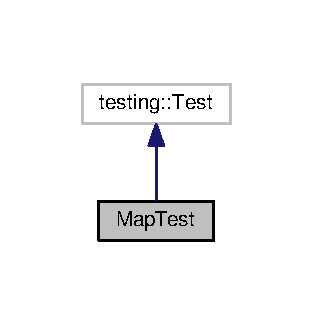
\includegraphics[width=150pt]{classMapTest__inherit__graph}
\end{center}
\end{figure}


Collaboration diagram for Map\-Test\-:
\nopagebreak
\begin{figure}[H]
\begin{center}
\leavevmode
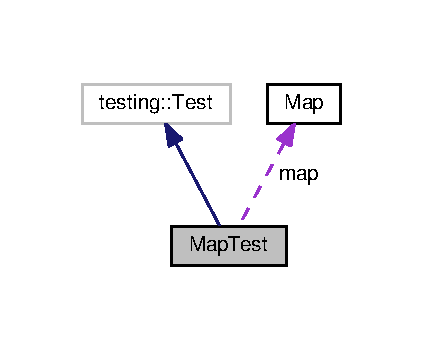
\includegraphics[width=203pt]{classMapTest__coll__graph}
\end{center}
\end{figure}
\subsection*{Public Member Functions}
\begin{DoxyCompactItemize}
\item 
\hypertarget{classMapTest_a494357a00f24b125e3b44bfebf0d4f9f}{void {\bfseries create\-Road} ()}\label{classMapTest_a494357a00f24b125e3b44bfebf0d4f9f}

\item 
\hypertarget{classMapTest_a6d77b0e6e116ddeff2813cea0a65600e}{void {\bfseries create\-Car} ()}\label{classMapTest_a6d77b0e6e116ddeff2813cea0a65600e}

\end{DoxyCompactItemize}
\subsection*{Public Attributes}
\begin{DoxyCompactItemize}
\item 
\hypertarget{classMapTest_afce2195037e3d9053a96b17ccc0cd6f8}{\hyperlink{classMap}{Map} {\bfseries map}}\label{classMapTest_afce2195037e3d9053a96b17ccc0cd6f8}

\end{DoxyCompactItemize}


The documentation for this class was generated from the following file\-:\begin{DoxyCompactItemize}
\item 
/home/aleksander/\-C\-Lion\-Projects/\-Zpr/test/Map\-Test.\-cpp\end{DoxyCompactItemize}

\hypertarget{classMovable}{\section{Movable Class Reference}
\label{classMovable}\index{Movable@{Movable}}
}


{\ttfamily \#include $<$Movable.\-h$>$}



Inheritance diagram for Movable\-:
\nopagebreak
\begin{figure}[H]
\begin{center}
\leavevmode
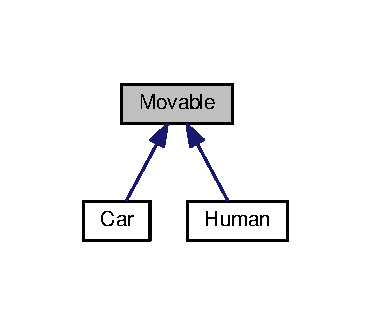
\includegraphics[width=178pt]{classMovable__inherit__graph}
\end{center}
\end{figure}
\subsection*{Public Member Functions}
\begin{DoxyCompactItemize}
\item 
bool \hyperlink{classMovable_afa3a7396ff6f8c5f5e51a0aeedfa332c}{move} ()
\item 
\hypertarget{classMovable_a03706cb151f6980ff79009749e26afe2}{\hyperlink{classPoint}{Point} {\bfseries get\-Actual\-Point} () const }\label{classMovable_a03706cb151f6980ff79009749e26afe2}

\item 
\hypertarget{classMovable_a5dbdb0881b07bff3faf68260bdb0b807}{unsigned int {\bfseries get\-Id} () const }\label{classMovable_a5dbdb0881b07bff3faf68260bdb0b807}

\item 
\hypertarget{classMovable_a1387ca11bd61513eb6e99d6ecd0b2de1}{bool {\bfseries is\-Fast} () const }\label{classMovable_a1387ca11bd61513eb6e99d6ecd0b2de1}

\end{DoxyCompactItemize}
\subsection*{Protected Member Functions}
\begin{DoxyCompactItemize}
\item 
\hypertarget{classMovable_a61c1152cca500d1f509afef590765ac7}{{\bfseries Movable} (\hyperlink{classRoute}{Route} $\ast$route, const \hyperlink{classPoint}{Point} \&actual\-Point, const int speed, const unsigned int id)}\label{classMovable_a61c1152cca500d1f509afef590765ac7}

\end{DoxyCompactItemize}


\subsection{Detailed Description}
Represents object that can move. \begin{DoxyAuthor}{Author}
Aleksander Brzozowski 
\end{DoxyAuthor}


\subsection{Member Function Documentation}
\hypertarget{classMovable_afa3a7396ff6f8c5f5e51a0aeedfa332c}{\index{Movable@{Movable}!move@{move}}
\index{move@{move}!Movable@{Movable}}
\subsubsection[{move}]{\setlength{\rightskip}{0pt plus 5cm}bool Movable\-::move (
\begin{DoxyParamCaption}
{}
\end{DoxyParamCaption}
)}}\label{classMovable_afa3a7396ff6f8c5f5e51a0aeedfa332c}
Moves movable. \begin{DoxyReturn}{Returns}
whether movable was moved 
\end{DoxyReturn}


The documentation for this class was generated from the following files\-:\begin{DoxyCompactItemize}
\item 
/home/aleksander/\-C\-Lion\-Projects/\-Zpr/src/Movable.\-h\item 
/home/aleksander/\-C\-Lion\-Projects/\-Zpr/src/Movable.\-cpp\end{DoxyCompactItemize}

\hypertarget{classMovableFactory}{\section{Movable\-Factory Class Reference}
\label{classMovableFactory}\index{Movable\-Factory@{Movable\-Factory}}
}


Factory of movables (cars and humans) with algorithms to finding routes.  




{\ttfamily \#include $<$Movable\-Factory.\-h$>$}

\subsection*{Public Member Functions}
\begin{DoxyCompactItemize}
\item 
void \hyperlink{classMovableFactory_a38bfc032a4e526e24b6dc186cda1382e}{find\-Route} (Ptr\-To\-Const\-Point, Ptr\-To\-Const\-Point, std\-::vector$<$ Ptr\-To\-Const\-Point $>$ \&, std\-::vector$<$ Ptr\-Cross $>$ \&)
\begin{DoxyCompactList}\small\item\em Finds route between two points on the map. \end{DoxyCompactList}\item 
void \hyperlink{classMovableFactory_addc3e4721ec280bafebd41332ef16a54}{prepare\-Route\-Finding} (std\-::vector$<$ Ptr\-Cross $>$ \&)
\begin{DoxyCompactList}\small\item\em Prepare crosses for running finding route algorithm. \end{DoxyCompactList}\item 
bool \hyperlink{classMovableFactory_a9f12c7d5c0cc67b8ad9a58a574b8427c}{point\-Meets\-Cross} (Ptr\-To\-Const\-Point, Ptr\-Cross) const 
\begin{DoxyCompactList}\small\item\em Checking if given point directly \char`\"{}sees\char`\"{} the given cross. \end{DoxyCompactList}\item 
Ptr\-Cross \hyperlink{classMovableFactory_a510b583ce682dec2d4e2988029b0c9ac}{find\-Nearest\-Cross} (Ptr\-To\-Const\-Point, const std\-::vector$<$ Ptr\-Cross $>$ \&) const 
\begin{DoxyCompactList}\small\item\em Looking for a cross that directly \char`\"{}sees\char`\"{} the given point. \end{DoxyCompactList}\item 
unsigned int \hyperlink{classMovableFactory_a3e6a2b041b143eee4b139001c0efb233}{get\-Movable\-Id} ()
\begin{DoxyCompactList}\small\item\em Get unique id for new movable. \end{DoxyCompactList}\item 
bool \hyperlink{classMovableFactory_a7947ef24e338a9c06145eb1665666ea3}{create\-Car} (Ptr\-To\-Const\-Point, Ptr\-To\-Const\-Point, int, std\-::vector$<$ Ptr\-Cross $>$ \&)
\begin{DoxyCompactList}\small\item\em Creating new car running from point to point at set speed. \end{DoxyCompactList}\item 
bool \hyperlink{classMovableFactory_a218fc6471b2d6d17c7d00697160f9d02}{create\-Human} (Ptr\-To\-Const\-Point, Ptr\-To\-Const\-Point, int, std\-::vector$<$ Ptr\-Cross $>$ \&)
\begin{DoxyCompactList}\small\item\em Creating new human running from point to point at set speed. \end{DoxyCompactList}\item 
void \hyperlink{classMovableFactory_a56b1d3085a535d40cfe4e6ef1f3ecf6e}{move\-Humans\-On\-Sidewalks} (std\-::vector$<$ Ptr\-To\-Const\-Point $>$ \&)
\begin{DoxyCompactList}\small\item\em Transforming found route for humans to be set on sidewalks. \end{DoxyCompactList}\item 
\hypertarget{classMovableFactory_a792ef3b707099931bfab7dddbd0b776b}{std\-::list$<$ Ptr\-Car $>$ \& {\bfseries get\-Cars} ()}\label{classMovableFactory_a792ef3b707099931bfab7dddbd0b776b}

\item 
\hypertarget{classMovableFactory_ae8c900bfd2548d7fd0e8f96f81fa7412}{std\-::list$<$ Ptr\-Human $>$ \& {\bfseries get\-Humans} ()}\label{classMovableFactory_ae8c900bfd2548d7fd0e8f96f81fa7412}

\end{DoxyCompactItemize}


\subsection{Detailed Description}
Factory of movables (cars and humans) with algorithms to finding routes. 

The factory prepares proper routes between given points for cars and humans. Cars have to run on streets. Humans have to walk on sidewalks. 

\subsection{Member Function Documentation}
\hypertarget{classMovableFactory_a7947ef24e338a9c06145eb1665666ea3}{\index{Movable\-Factory@{Movable\-Factory}!create\-Car@{create\-Car}}
\index{create\-Car@{create\-Car}!MovableFactory@{Movable\-Factory}}
\subsubsection[{create\-Car}]{\setlength{\rightskip}{0pt plus 5cm}bool Movable\-Factory\-::create\-Car (
\begin{DoxyParamCaption}
\item[{Ptr\-To\-Const\-Point}]{src, }
\item[{Ptr\-To\-Const\-Point}]{dst, }
\item[{int}]{speed, }
\item[{std\-::vector$<$ Ptr\-Cross $>$ \&}]{crosses}
\end{DoxyParamCaption}
)}}\label{classMovableFactory_a7947ef24e338a9c06145eb1665666ea3}


Creating new car running from point to point at set speed. 

Method at first looks for a route between starting and ending points. If route was found, creates car and includes it to the simulation. 
\begin{DoxyParams}{Parameters}
{\em src} & as shared\-\_\-ptr to const \hyperlink{classPoint}{Point} type object, starting point of the car's route. \\
\hline
{\em dst} & as shared\-\_\-ptr to const \hyperlink{classPoint}{Point} type object, ending point of the car's route. \\
\hline
{\em speed} & integer argument, speed of car. \\
\hline
{\em crosses} & vector of shared\-\_\-ptr to Crosses type objects, needed to make routes for cars. \\
\hline
\end{DoxyParams}
\begin{DoxyReturn}{Returns}
true if route between starting and ending points was found and car was created. 
\end{DoxyReturn}
\hypertarget{classMovableFactory_a218fc6471b2d6d17c7d00697160f9d02}{\index{Movable\-Factory@{Movable\-Factory}!create\-Human@{create\-Human}}
\index{create\-Human@{create\-Human}!MovableFactory@{Movable\-Factory}}
\subsubsection[{create\-Human}]{\setlength{\rightskip}{0pt plus 5cm}bool Movable\-Factory\-::create\-Human (
\begin{DoxyParamCaption}
\item[{Ptr\-To\-Const\-Point}]{src, }
\item[{Ptr\-To\-Const\-Point}]{dst, }
\item[{int}]{speed, }
\item[{std\-::vector$<$ Ptr\-Cross $>$ \&}]{crosses}
\end{DoxyParamCaption}
)}}\label{classMovableFactory_a218fc6471b2d6d17c7d00697160f9d02}


Creating new human running from point to point at set speed. 

Method at first looks for a route between starting and ending points. If route was found, creates human and includes it to the simulation. 
\begin{DoxyParams}{Parameters}
{\em src} & as shared\-\_\-ptr to const \hyperlink{classPoint}{Point} type object, starting point of the human's route. \\
\hline
{\em dst} & as shared\-\_\-ptr to const \hyperlink{classPoint}{Point} type object, ending point of the human's route. \\
\hline
{\em speed} & integer argument, speed of human. \\
\hline
{\em crosses} & vector of shared\-\_\-ptr to Crosses type objects, needed to make routes for humans. \\
\hline
\end{DoxyParams}
\begin{DoxyReturn}{Returns}
true if route between starting and ending points was found and human was created. 
\end{DoxyReturn}
\hypertarget{classMovableFactory_a510b583ce682dec2d4e2988029b0c9ac}{\index{Movable\-Factory@{Movable\-Factory}!find\-Nearest\-Cross@{find\-Nearest\-Cross}}
\index{find\-Nearest\-Cross@{find\-Nearest\-Cross}!MovableFactory@{Movable\-Factory}}
\subsubsection[{find\-Nearest\-Cross}]{\setlength{\rightskip}{0pt plus 5cm}Ptr\-Cross Movable\-Factory\-::find\-Nearest\-Cross (
\begin{DoxyParamCaption}
\item[{Ptr\-To\-Const\-Point}]{point, }
\item[{const std\-::vector$<$ Ptr\-Cross $>$ \&}]{crosses}
\end{DoxyParamCaption}
) const}}\label{classMovableFactory_a510b583ce682dec2d4e2988029b0c9ac}


Looking for a cross that directly \char`\"{}sees\char`\"{} the given point. 

Finds the cross that has direct route to the given point. 
\begin{DoxyParams}{Parameters}
{\em point} & as shared\-\_\-ptr$<$\-Point$>$, given point. \\
\hline
{\em crosses} & as vector of shared\-\_\-ptr$<$\-Cross$>$ consisting of every existing crosses. \\
\hline
\end{DoxyParams}
\begin{DoxyReturn}{Returns}
shared\-\_\-ptr$<$\-Cross$>$ of the cross that directly \char`\"{}sees\char`\"{} the given point. 
\end{DoxyReturn}
\hypertarget{classMovableFactory_a38bfc032a4e526e24b6dc186cda1382e}{\index{Movable\-Factory@{Movable\-Factory}!find\-Route@{find\-Route}}
\index{find\-Route@{find\-Route}!MovableFactory@{Movable\-Factory}}
\subsubsection[{find\-Route}]{\setlength{\rightskip}{0pt plus 5cm}void Movable\-Factory\-::find\-Route (
\begin{DoxyParamCaption}
\item[{Ptr\-To\-Const\-Point}]{src, }
\item[{Ptr\-To\-Const\-Point}]{dst, }
\item[{std\-::vector$<$ Ptr\-To\-Const\-Point $>$ \&}]{ready\-Route, }
\item[{std\-::vector$<$ Ptr\-Cross $>$ \&}]{crosses}
\end{DoxyParamCaption}
)}}\label{classMovableFactory_a38bfc032a4e526e24b6dc186cda1382e}


Finds route between two points on the map. 

Finding route between starting point and ending point. Finding route algorithm runs similar to the D\-F\-S algorithm in graph (map). 
\begin{DoxyParams}{Parameters}
{\em src} & starting point as shared\-\_\-ptr$<$\-Point$>$. \\
\hline
{\em dst} & endign point as shared\-\_\-ptr$<$\-Point$>$. \\
\hline
{\em ready\-Route} & vector to which new points will be written. \\
\hline
{\em crosses} & vector of crosses to find route. \\
\hline
\end{DoxyParams}
\hypertarget{classMovableFactory_a3e6a2b041b143eee4b139001c0efb233}{\index{Movable\-Factory@{Movable\-Factory}!get\-Movable\-Id@{get\-Movable\-Id}}
\index{get\-Movable\-Id@{get\-Movable\-Id}!MovableFactory@{Movable\-Factory}}
\subsubsection[{get\-Movable\-Id}]{\setlength{\rightskip}{0pt plus 5cm}unsigned int Movable\-Factory\-::get\-Movable\-Id (
\begin{DoxyParamCaption}
{}
\end{DoxyParamCaption}
)}}\label{classMovableFactory_a3e6a2b041b143eee4b139001c0efb233}


Get unique id for new movable. 

\begin{DoxyReturn}{Returns}
new Id for movables. 
\end{DoxyReturn}
\hypertarget{classMovableFactory_a56b1d3085a535d40cfe4e6ef1f3ecf6e}{\index{Movable\-Factory@{Movable\-Factory}!move\-Humans\-On\-Sidewalks@{move\-Humans\-On\-Sidewalks}}
\index{move\-Humans\-On\-Sidewalks@{move\-Humans\-On\-Sidewalks}!MovableFactory@{Movable\-Factory}}
\subsubsection[{move\-Humans\-On\-Sidewalks}]{\setlength{\rightskip}{0pt plus 5cm}void Movable\-Factory\-::move\-Humans\-On\-Sidewalks (
\begin{DoxyParamCaption}
\item[{std\-::vector$<$ Ptr\-To\-Const\-Point $>$ \&}]{route}
\end{DoxyParamCaption}
)}}\label{classMovableFactory_a56b1d3085a535d40cfe4e6ef1f3ecf6e}


Transforming found route for humans to be set on sidewalks. 

Adding offset between the street and sidewalk to every point in the found route to make humans walking on the sidewalks. 
\begin{DoxyParams}{Parameters}
{\em route} & as vector of shared\-\_\-ptr to const \hyperlink{classPoint}{Point} type objects to add to each point offset between street and sidewalk. \\
\hline
\end{DoxyParams}
\hypertarget{classMovableFactory_a9f12c7d5c0cc67b8ad9a58a574b8427c}{\index{Movable\-Factory@{Movable\-Factory}!point\-Meets\-Cross@{point\-Meets\-Cross}}
\index{point\-Meets\-Cross@{point\-Meets\-Cross}!MovableFactory@{Movable\-Factory}}
\subsubsection[{point\-Meets\-Cross}]{\setlength{\rightskip}{0pt plus 5cm}bool Movable\-Factory\-::point\-Meets\-Cross (
\begin{DoxyParamCaption}
\item[{Ptr\-To\-Const\-Point}]{point, }
\item[{Ptr\-Cross}]{cross}
\end{DoxyParamCaption}
) const}}\label{classMovableFactory_a9f12c7d5c0cc67b8ad9a58a574b8427c}


Checking if given point directly \char`\"{}sees\char`\"{} the given cross. 

Checking if point has direct route to the given cross (without any crosses (on the way). 
\begin{DoxyParams}{Parameters}
{\em point} & as shared\-\_\-ptr$<$\-Point$>$, which point we want to check. \\
\hline
{\em cross} & as shared\-\_\-ptr$<$\-Cross$>$, which cross we want to check. \\
\hline
\end{DoxyParams}
\begin{DoxyReturn}{Returns}
true if given point has direct route to given cross. 
\end{DoxyReturn}
\hypertarget{classMovableFactory_addc3e4721ec280bafebd41332ef16a54}{\index{Movable\-Factory@{Movable\-Factory}!prepare\-Route\-Finding@{prepare\-Route\-Finding}}
\index{prepare\-Route\-Finding@{prepare\-Route\-Finding}!MovableFactory@{Movable\-Factory}}
\subsubsection[{prepare\-Route\-Finding}]{\setlength{\rightskip}{0pt plus 5cm}void Movable\-Factory\-::prepare\-Route\-Finding (
\begin{DoxyParamCaption}
\item[{std\-::vector$<$ Ptr\-Cross $>$ \&}]{crosses}
\end{DoxyParamCaption}
)}}\label{classMovableFactory_addc3e4721ec280bafebd41332ef16a54}


Prepare crosses for running finding route algorithm. 

Preparing crosses to be used by the finding route algorithm. 
\begin{DoxyParams}{Parameters}
{\em crosses} & to change crosses parameter. \\
\hline
\end{DoxyParams}


The documentation for this class was generated from the following files\-:\begin{DoxyCompactItemize}
\item 
/home/aleksander/\-C\-Lion\-Projects/\-Zpr/src/\hyperlink{MovableFactory_8h}{Movable\-Factory.\-h}\item 
/home/aleksander/\-C\-Lion\-Projects/\-Zpr/src/\hyperlink{MovableFactory_8cpp}{Movable\-Factory.\-cpp}\end{DoxyCompactItemize}

\hypertarget{classMovableFactoryTest}{\section{Movable\-Factory\-Test Class Reference}
\label{classMovableFactoryTest}\index{Movable\-Factory\-Test@{Movable\-Factory\-Test}}
}


Inheritance diagram for Movable\-Factory\-Test\-:
\nopagebreak
\begin{figure}[H]
\begin{center}
\leavevmode
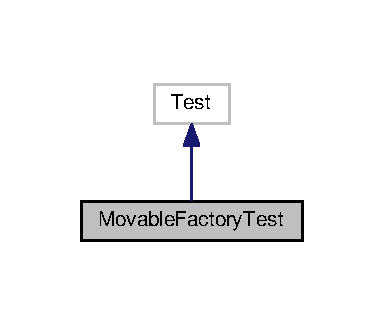
\includegraphics[width=184pt]{classMovableFactoryTest__inherit__graph}
\end{center}
\end{figure}


Collaboration diagram for Movable\-Factory\-Test\-:
\nopagebreak
\begin{figure}[H]
\begin{center}
\leavevmode
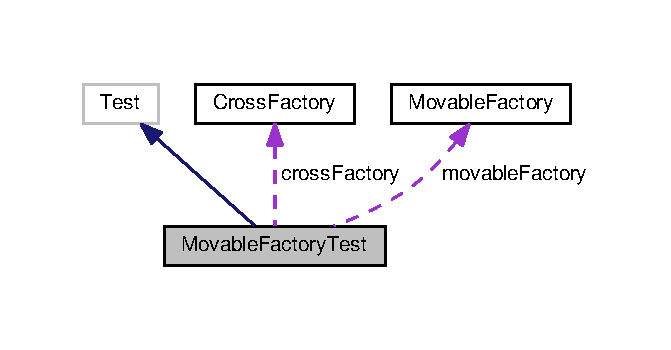
\includegraphics[width=322pt]{classMovableFactoryTest__coll__graph}
\end{center}
\end{figure}
\subsection*{Public Member Functions}
\begin{DoxyCompactItemize}
\item 
\hypertarget{classMovableFactoryTest_ac204d112e5b47b9de00e0a349fef3c90}{void {\bfseries create\-Crosses} ()}\label{classMovableFactoryTest_ac204d112e5b47b9de00e0a349fef3c90}

\end{DoxyCompactItemize}
\subsection*{Public Attributes}
\begin{DoxyCompactItemize}
\item 
\hypertarget{classMovableFactoryTest_a7258af44f525ddbf48ec2e6b3276a2db}{\hyperlink{classMovableFactory}{Movable\-Factory} {\bfseries movable\-Factory}}\label{classMovableFactoryTest_a7258af44f525ddbf48ec2e6b3276a2db}

\item 
\hypertarget{classMovableFactoryTest_abc919e5227b34cfb45bfd20c7be038b0}{\hyperlink{classCrossFactory}{Cross\-Factory} {\bfseries cross\-Factory}}\label{classMovableFactoryTest_abc919e5227b34cfb45bfd20c7be038b0}

\end{DoxyCompactItemize}


The documentation for this class was generated from the following file\-:\begin{DoxyCompactItemize}
\item 
/home/aleksander/\-C\-Lion\-Projects/\-Zpr/test/Movable\-Factory\-Test.\-cpp\end{DoxyCompactItemize}

\hypertarget{classPoint}{\section{Point Class Reference}
\label{classPoint}\index{Point@{Point}}
}


{\ttfamily \#include $<$Point.\-h$>$}

\subsection*{Public Member Functions}
\begin{DoxyCompactItemize}
\item 
\hyperlink{classPoint_a001c4958c310b248f5c26037aea38a9c}{Point} (int x, int y)
\item 
\hyperlink{classPoint_ad92f2337b839a94ce97dcdb439b4325a}{Point} ()
\item 
\hyperlink{classPoint_a53534941e7bcb3c6d3af84d58a542899}{Point} (const \hyperlink{classPoint}{Point} \&point)
\item 
\hypertarget{classPoint_abe622fffc8785b0c2e06cdac681b9837}{int {\bfseries get\-X} () const }\label{classPoint_abe622fffc8785b0c2e06cdac681b9837}

\item 
\hypertarget{classPoint_acdc86ab607b2ae8415152883e2629015}{void {\bfseries set\-X} (int x)}\label{classPoint_acdc86ab607b2ae8415152883e2629015}

\item 
\hypertarget{classPoint_a10f31e48e2dbc22e3660ca769b8d5d65}{int {\bfseries get\-Y} () const }\label{classPoint_a10f31e48e2dbc22e3660ca769b8d5d65}

\item 
\hypertarget{classPoint_afccad787a359f062efc1af5e935a99ba}{void {\bfseries set\-Y} (int y)}\label{classPoint_afccad787a359f062efc1af5e935a99ba}

\item 
\hypertarget{classPoint_a381c5b2ac13d8a3966f5225f94fff6fa}{bool {\bfseries operator==} (const \hyperlink{classPoint}{Point} \&rhs) const }\label{classPoint_a381c5b2ac13d8a3966f5225f94fff6fa}

\item 
\hypertarget{classPoint_aa85f211e55420f0f622a77920581732a}{bool {\bfseries operator!=} (const \hyperlink{classPoint}{Point} \&rhs) const }\label{classPoint_aa85f211e55420f0f622a77920581732a}

\item 
\hypertarget{classPoint_aaea5d476866984dc521991e606040b52}{\hyperlink{classPoint}{Point} \& {\bfseries operator-\/=} (const \hyperlink{classPoint}{Point} \&rhs)}\label{classPoint_aaea5d476866984dc521991e606040b52}

\item 
\hypertarget{classPoint_a7421422b4e45c5569b9a0e981a7ab735}{\hyperlink{classPoint}{Point} \& {\bfseries operator+=} (const \hyperlink{classPoint}{Point} \&rhs)}\label{classPoint_a7421422b4e45c5569b9a0e981a7ab735}

\item 
\hypertarget{classPoint_a15d86ccf688d17948f2d16634151bd24}{const \hyperlink{classPoint}{Point} {\bfseries operator-\/} (const \hyperlink{classPoint}{Point} \&rhs) const }\label{classPoint_a15d86ccf688d17948f2d16634151bd24}

\item 
\hypertarget{classPoint_afad60ddeb82566a93079071e5802147c}{const \hyperlink{classPoint}{Point} {\bfseries operator+} (const \hyperlink{classPoint}{Point} \&rhs) const }\label{classPoint_afad60ddeb82566a93079071e5802147c}

\end{DoxyCompactItemize}
\subsection*{Friends}
\begin{DoxyCompactItemize}
\item 
\hypertarget{classPoint_a97713abf198b35c58044f2c4d04a19ea}{std\-::ostream \& {\bfseries operator$<$$<$} (std\-::ostream \&os, const \hyperlink{classPoint}{Point} \&point)}\label{classPoint_a97713abf198b35c58044f2c4d04a19ea}

\end{DoxyCompactItemize}


\subsection{Detailed Description}
Represents 2-\/\-D point. \begin{DoxyAuthor}{Author}
Aleksander Brzozowski 
\end{DoxyAuthor}


\subsection{Constructor \& Destructor Documentation}
\hypertarget{classPoint_a001c4958c310b248f5c26037aea38a9c}{\index{Point@{Point}!Point@{Point}}
\index{Point@{Point}!Point@{Point}}
\subsubsection[{Point}]{\setlength{\rightskip}{0pt plus 5cm}Point\-::\-Point (
\begin{DoxyParamCaption}
\item[{int}]{x, }
\item[{int}]{y}
\end{DoxyParamCaption}
)}}\label{classPoint_a001c4958c310b248f5c26037aea38a9c}
Constructs point using passed x and y (x, y). 
\begin{DoxyParams}{Parameters}
{\em x} & \hyperlink{classPoint}{Point}'s x \\
\hline
{\em y} & \hyperlink{classPoint}{Point}'s y \\
\hline
\end{DoxyParams}
\hypertarget{classPoint_ad92f2337b839a94ce97dcdb439b4325a}{\index{Point@{Point}!Point@{Point}}
\index{Point@{Point}!Point@{Point}}
\subsubsection[{Point}]{\setlength{\rightskip}{0pt plus 5cm}Point\-::\-Point (
\begin{DoxyParamCaption}
{}
\end{DoxyParamCaption}
)}}\label{classPoint_ad92f2337b839a94ce97dcdb439b4325a}
Constructs point (0, 0) \hypertarget{classPoint_a53534941e7bcb3c6d3af84d58a542899}{\index{Point@{Point}!Point@{Point}}
\index{Point@{Point}!Point@{Point}}
\subsubsection[{Point}]{\setlength{\rightskip}{0pt plus 5cm}Point\-::\-Point (
\begin{DoxyParamCaption}
\item[{const {\bf Point} \&}]{point}
\end{DoxyParamCaption}
)}}\label{classPoint_a53534941e7bcb3c6d3af84d58a542899}
Constructs shallow copy of passed point. 
\begin{DoxyParams}{Parameters}
{\em point} & Used point to create copy \\
\hline
\end{DoxyParams}


The documentation for this class was generated from the following files\-:\begin{DoxyCompactItemize}
\item 
/home/aleksander/\-C\-Lion\-Projects/\-Zpr/src/Point.\-h\item 
/home/aleksander/\-C\-Lion\-Projects/\-Zpr/src/Point.\-cpp\end{DoxyCompactItemize}

\hypertarget{classPplGUI}{\section{Ppl\-G\-U\-I Class Reference}
\label{classPplGUI}\index{Ppl\-G\-U\-I@{Ppl\-G\-U\-I}}
}


The \hyperlink{classPplGUI}{Ppl\-G\-U\-I} class.  




{\ttfamily \#include $<$pplgui.\-h$>$}



Inheritance diagram for Ppl\-G\-U\-I\-:
\nopagebreak
\begin{figure}[H]
\begin{center}
\leavevmode
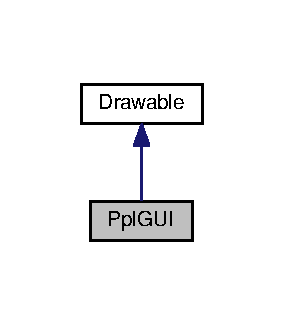
\includegraphics[width=136pt]{classPplGUI__inherit__graph}
\end{center}
\end{figure}


Collaboration diagram for Ppl\-G\-U\-I\-:
\nopagebreak
\begin{figure}[H]
\begin{center}
\leavevmode
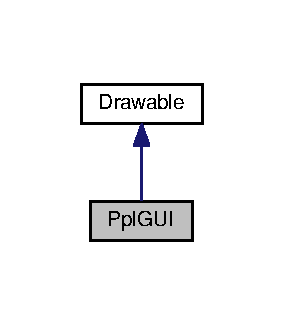
\includegraphics[width=136pt]{classPplGUI__coll__graph}
\end{center}
\end{figure}
\subsection*{Public Member Functions}
\begin{DoxyCompactItemize}
\item 
\hyperlink{classPplGUI_a575f17881dcc07898b3f61f5a1a48ac3}{Ppl\-G\-U\-I} (Q\-Rect ppl\-Rect, bool ghost=false)
\begin{DoxyCompactList}\small\item\em \hyperlink{classPplGUI_a575f17881dcc07898b3f61f5a1a48ac3}{Ppl\-G\-U\-I\-::\-Ppl\-G\-U\-I}. Constructor. \end{DoxyCompactList}\item 
\hyperlink{classPplGUI_ad03566a9fb76c98e1490372292fea344}{Ppl\-G\-U\-I} (unsigned int x, unsigned int y, bool ghost=false)
\begin{DoxyCompactList}\small\item\em \hyperlink{classPplGUI_a575f17881dcc07898b3f61f5a1a48ac3}{Ppl\-G\-U\-I\-::\-Ppl\-G\-U\-I}. Constructor. \end{DoxyCompactList}\item 
void \hyperlink{classPplGUI_a454ea7b7efa82f9bdd383cb70021c23b}{draw} (Q\-Painter \&painter) const override
\begin{DoxyCompactList}\small\item\em \hyperlink{classPplGUI_a454ea7b7efa82f9bdd383cb70021c23b}{Ppl\-G\-U\-I\-::draw}. \end{DoxyCompactList}\item 
void \hyperlink{classPplGUI_a9239f31269b63e32540c588736520e3c}{set\-To} (unsigned int x, unsigned int y) override
\begin{DoxyCompactList}\small\item\em \hyperlink{classPplGUI_a9239f31269b63e32540c588736520e3c}{Ppl\-G\-U\-I\-::set\-To}. \end{DoxyCompactList}\item 
bool \hyperlink{classPplGUI_aad8337d505325dcb8d16aa1ce31b76f9}{intersects} (Q\-Rect \&rectangle) const override
\begin{DoxyCompactList}\small\item\em \hyperlink{classPplGUI_aad8337d505325dcb8d16aa1ce31b76f9}{Ppl\-G\-U\-I\-::intersects}. \end{DoxyCompactList}\end{DoxyCompactItemize}
\subsection*{Static Public Attributes}
\begin{DoxyCompactItemize}
\item 
static const int \hyperlink{classPplGUI_aa86753ab1d23b8aaa73f9fc20ca75449}{R\-A\-D\-I\-U\-S} = 5
\item 
\hypertarget{classPplGUI_a472efdfe83788f4b6e51f82b6d4fea1d}{static const int {\bfseries P\-E\-N\-\_\-\-W\-I\-D\-T\-H} = 2}\label{classPplGUI_a472efdfe83788f4b6e51f82b6d4fea1d}

\item 
\hypertarget{classPplGUI_a84984104fb0e25bfd7e15e7e55b6bae7}{static const Qt\-::\-Pen\-Style {\bfseries P\-E\-N\-\_\-\-S\-T\-Y\-L\-E} = Qt\-::\-Solid\-Line}\label{classPplGUI_a84984104fb0e25bfd7e15e7e55b6bae7}

\item 
\hypertarget{classPplGUI_aa62278888ec92a1c333eae538f4f6f3f}{static const Qt\-::\-Pen\-Cap\-Style {\bfseries P\-E\-N\-\_\-\-C\-A\-P} = Qt\-::\-Square\-Cap}\label{classPplGUI_aa62278888ec92a1c333eae538f4f6f3f}

\item 
\hypertarget{classPplGUI_a4d60f70be938573fa65312c1809dea4b}{static const Qt\-::\-Pen\-Join\-Style {\bfseries P\-E\-N\-\_\-\-J\-O\-I\-N} = Qt\-::\-Round\-Join}\label{classPplGUI_a4d60f70be938573fa65312c1809dea4b}

\item 
\hypertarget{classPplGUI_aacdfeb01d44ed21ad38850114ecfd351}{static const Q\-Color {\bfseries P\-E\-N\-\_\-\-C\-O\-L\-O\-R} = Qt\-::black}\label{classPplGUI_aacdfeb01d44ed21ad38850114ecfd351}

\item 
\hypertarget{classPplGUI_a582ad86f1d58b82abcd0c668ed851100}{static const Q\-Color {\bfseries G\-H\-O\-S\-T\-\_\-\-P\-E\-N\-\_\-\-C\-O\-L\-O\-R} = Q\-Color(0, 0, 0, 127)}\label{classPplGUI_a582ad86f1d58b82abcd0c668ed851100}

\item 
\hypertarget{classPplGUI_a349527436240716995da703c6bf6f40f}{static const Q\-Pen {\bfseries P\-E\-N}}\label{classPplGUI_a349527436240716995da703c6bf6f40f}

\item 
\hypertarget{classPplGUI_a66c4ea9d3d59218dca5d7b6679ddb2e6}{static const Q\-Pen {\bfseries G\-H\-O\-S\-T\-\_\-\-P\-E\-N}}\label{classPplGUI_a66c4ea9d3d59218dca5d7b6679ddb2e6}

\item 
\hypertarget{classPplGUI_a182d5e147d9dab40810270b6eee13e29}{static const Qt\-::\-Brush\-Style {\bfseries B\-R\-U\-S\-H\-\_\-\-S\-T\-Y\-L\-E} = Qt\-::\-Solid\-Pattern}\label{classPplGUI_a182d5e147d9dab40810270b6eee13e29}

\item 
\hypertarget{classPplGUI_a9a5acb61b9f5b566250ba23145e12eb8}{static const Q\-Color {\bfseries B\-R\-U\-S\-H\-\_\-\-C\-O\-L\-O\-R} = Q\-Color(255, 105, 97)}\label{classPplGUI_a9a5acb61b9f5b566250ba23145e12eb8}

\item 
\hypertarget{classPplGUI_a79c19c75f04e710dfe287988fd687d64}{static const Q\-Color {\bfseries G\-H\-O\-S\-T\-\_\-\-B\-R\-U\-S\-H\-\_\-\-C\-O\-L\-O\-R} = Q\-Color(255, 105, 97, 127)}\label{classPplGUI_a79c19c75f04e710dfe287988fd687d64}

\item 
\hypertarget{classPplGUI_a478a2211e66aedeb3dba7c8ed4f1d16f}{static const Q\-Brush {\bfseries B\-R\-U\-S\-H}}\label{classPplGUI_a478a2211e66aedeb3dba7c8ed4f1d16f}

\item 
\hypertarget{classPplGUI_a28b6b84e45eecb95a57fd6ccbb83dd32}{static const Q\-Brush {\bfseries G\-H\-O\-S\-T\-\_\-\-B\-R\-U\-S\-H}}\label{classPplGUI_a28b6b84e45eecb95a57fd6ccbb83dd32}

\item 
\hypertarget{classPplGUI_a9bea7d41fbb3a003d6b8e7350f3e3508}{static const int {\bfseries S\-P\-E\-E\-D} = 1}\label{classPplGUI_a9bea7d41fbb3a003d6b8e7350f3e3508}

\item 
\hypertarget{classPplGUI_aef4e28993788ca773cecd5aa091d2248}{static const int {\bfseries O\-F\-F\-S\-E\-T} = Grid\-G\-U\-I\-::\-S\-I\-Z\-E/2 -\/ Road\-G\-U\-I\-::\-S\-I\-D\-E\-W\-A\-L\-K\-\_\-\-W\-I\-D\-T\-H/2}\label{classPplGUI_aef4e28993788ca773cecd5aa091d2248}

\end{DoxyCompactItemize}


\subsection{Detailed Description}
The \hyperlink{classPplGUI}{Ppl\-G\-U\-I} class. 

Class holds all necessary information to draw \hyperlink{classHuman}{Human} object on screen. It implements functions from base class thar defines how \hyperlink{classHuman}{Human} will look. It also holds all variables that define look of the \hyperlink{classHuman}{Human} object on screen. \begin{DoxyAuthor}{Author}
Pawel Rybak 
\end{DoxyAuthor}


\subsection{Constructor \& Destructor Documentation}
\hypertarget{classPplGUI_a575f17881dcc07898b3f61f5a1a48ac3}{\index{Ppl\-G\-U\-I@{Ppl\-G\-U\-I}!Ppl\-G\-U\-I@{Ppl\-G\-U\-I}}
\index{Ppl\-G\-U\-I@{Ppl\-G\-U\-I}!PplGUI@{Ppl\-G\-U\-I}}
\subsubsection[{Ppl\-G\-U\-I}]{\setlength{\rightskip}{0pt plus 5cm}Ppl\-G\-U\-I\-::\-Ppl\-G\-U\-I (
\begin{DoxyParamCaption}
\item[{Q\-Rect}]{ppl\-Rect, }
\item[{bool}]{ghost = {\ttfamily false}}
\end{DoxyParamCaption}
)}}\label{classPplGUI_a575f17881dcc07898b3f61f5a1a48ac3}


\hyperlink{classPplGUI_a575f17881dcc07898b3f61f5a1a48ac3}{Ppl\-G\-U\-I\-::\-Ppl\-G\-U\-I}. Constructor. 


\begin{DoxyParams}{Parameters}
{\em ppl\-Rect} & -\/ Rectangle in which human object will be drawn. \\
\hline
{\em ghost} & -\/ Bool flag tells whether object is ghost object.\\
\hline
\end{DoxyParams}
Constructs human visualization object based on Q\-Rect object given as argument. \hypertarget{classPplGUI_ad03566a9fb76c98e1490372292fea344}{\index{Ppl\-G\-U\-I@{Ppl\-G\-U\-I}!Ppl\-G\-U\-I@{Ppl\-G\-U\-I}}
\index{Ppl\-G\-U\-I@{Ppl\-G\-U\-I}!PplGUI@{Ppl\-G\-U\-I}}
\subsubsection[{Ppl\-G\-U\-I}]{\setlength{\rightskip}{0pt plus 5cm}Ppl\-G\-U\-I\-::\-Ppl\-G\-U\-I (
\begin{DoxyParamCaption}
\item[{unsigned int}]{x, }
\item[{unsigned int}]{y, }
\item[{bool}]{ghost = {\ttfamily false}}
\end{DoxyParamCaption}
)}}\label{classPplGUI_ad03566a9fb76c98e1490372292fea344}


\hyperlink{classPplGUI_a575f17881dcc07898b3f61f5a1a48ac3}{Ppl\-G\-U\-I\-::\-Ppl\-G\-U\-I}. Constructor. 


\begin{DoxyParams}{Parameters}
{\em x} & -\/ Position X of human. \\
\hline
{\em y} & -\/ Position Y of human. \\
\hline
{\em ghost} & -\/ Bool flag tells whether object is ghost object.\\
\hline
\end{DoxyParams}
Constructs human visualization based on X and Y position given as arguments. 

\subsection{Member Function Documentation}
\hypertarget{classPplGUI_a454ea7b7efa82f9bdd383cb70021c23b}{\index{Ppl\-G\-U\-I@{Ppl\-G\-U\-I}!draw@{draw}}
\index{draw@{draw}!PplGUI@{Ppl\-G\-U\-I}}
\subsubsection[{draw}]{\setlength{\rightskip}{0pt plus 5cm}void Ppl\-G\-U\-I\-::draw (
\begin{DoxyParamCaption}
\item[{Q\-Painter \&}]{painter}
\end{DoxyParamCaption}
) const\hspace{0.3cm}{\ttfamily [override]}, {\ttfamily [virtual]}}}\label{classPplGUI_a454ea7b7efa82f9bdd383cb70021c23b}


\hyperlink{classPplGUI_a454ea7b7efa82f9bdd383cb70021c23b}{Ppl\-G\-U\-I\-::draw}. 


\begin{DoxyParams}{Parameters}
{\em painter} & -\/ Reference to painter object.\\
\hline
\end{DoxyParams}
Function draws object using painter given as an arrgument. It uses brushes and pens defined in object, and base its choice on whether object is ghost object or not. 

Implements \hyperlink{classDrawable}{Drawable}.

\hypertarget{classPplGUI_aad8337d505325dcb8d16aa1ce31b76f9}{\index{Ppl\-G\-U\-I@{Ppl\-G\-U\-I}!intersects@{intersects}}
\index{intersects@{intersects}!PplGUI@{Ppl\-G\-U\-I}}
\subsubsection[{intersects}]{\setlength{\rightskip}{0pt plus 5cm}bool Ppl\-G\-U\-I\-::intersects (
\begin{DoxyParamCaption}
\item[{Q\-Rect \&}]{rectangle}
\end{DoxyParamCaption}
) const\hspace{0.3cm}{\ttfamily [override]}, {\ttfamily [virtual]}}}\label{classPplGUI_aad8337d505325dcb8d16aa1ce31b76f9}


\hyperlink{classPplGUI_aad8337d505325dcb8d16aa1ce31b76f9}{Ppl\-G\-U\-I\-::intersects}. 


\begin{DoxyParams}{Parameters}
{\em rectangle} & -\/ Q\-Rect object that is being checked for intersection. \\
\hline
\end{DoxyParams}
\begin{DoxyReturn}{Returns}
Bool value whether rectangles intersects.
\end{DoxyReturn}
Function checks whether current object's rectangle and rectangle given as argument intersects and returns bool value. 

Implements \hyperlink{classDrawable}{Drawable}.

\hypertarget{classPplGUI_a9239f31269b63e32540c588736520e3c}{\index{Ppl\-G\-U\-I@{Ppl\-G\-U\-I}!set\-To@{set\-To}}
\index{set\-To@{set\-To}!PplGUI@{Ppl\-G\-U\-I}}
\subsubsection[{set\-To}]{\setlength{\rightskip}{0pt plus 5cm}void Ppl\-G\-U\-I\-::set\-To (
\begin{DoxyParamCaption}
\item[{unsigned int}]{x, }
\item[{unsigned int}]{y}
\end{DoxyParamCaption}
)\hspace{0.3cm}{\ttfamily [override]}, {\ttfamily [virtual]}}}\label{classPplGUI_a9239f31269b63e32540c588736520e3c}


\hyperlink{classPplGUI_a9239f31269b63e32540c588736520e3c}{Ppl\-G\-U\-I\-::set\-To}. 


\begin{DoxyParams}{Parameters}
{\em x} & -\/ New X position. \\
\hline
{\em y} & -\/ New Y positoin.\\
\hline
\end{DoxyParams}
Method moves human to position given with x and y arguments. Position given as arguments is center of object. 

Implements \hyperlink{classDrawable}{Drawable}.



\subsection{Member Data Documentation}
\hypertarget{classPplGUI_aa86753ab1d23b8aaa73f9fc20ca75449}{\index{Ppl\-G\-U\-I@{Ppl\-G\-U\-I}!R\-A\-D\-I\-U\-S@{R\-A\-D\-I\-U\-S}}
\index{R\-A\-D\-I\-U\-S@{R\-A\-D\-I\-U\-S}!PplGUI@{Ppl\-G\-U\-I}}
\subsubsection[{R\-A\-D\-I\-U\-S}]{\setlength{\rightskip}{0pt plus 5cm}const int Ppl\-G\-U\-I\-::\-R\-A\-D\-I\-U\-S = 5\hspace{0.3cm}{\ttfamily [static]}}}\label{classPplGUI_aa86753ab1d23b8aaa73f9fc20ca75449}
P\-R\-O\-P\-E\-R\-T\-I\-E\-S

P\-R\-O\-P\-E\-R\-T\-I\-E\-S I\-N\-I\-T\-I\-A\-L\-I\-Z\-A\-T\-I\-O\-N 

The documentation for this class was generated from the following files\-:\begin{DoxyCompactItemize}
\item 
/home/aleksander/\-C\-Lion\-Projects/\-Zpr/src/\-G\-U\-I/pplgui.\-h\item 
/home/aleksander/\-C\-Lion\-Projects/\-Zpr/src/\-G\-U\-I/pplgui.\-cpp\end{DoxyCompactItemize}

\hypertarget{classRoadGUI}{\section{Road\-G\-U\-I Class Reference}
\label{classRoadGUI}\index{Road\-G\-U\-I@{Road\-G\-U\-I}}
}


The \hyperlink{classRoadGUI}{Road\-G\-U\-I} class. Class holds info about look of roads in G\-U\-I.  




{\ttfamily \#include $<$roadgui.\-h$>$}



Inheritance diagram for Road\-G\-U\-I\-:
\nopagebreak
\begin{figure}[H]
\begin{center}
\leavevmode
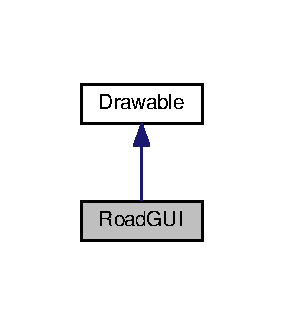
\includegraphics[width=136pt]{classRoadGUI__inherit__graph}
\end{center}
\end{figure}


Collaboration diagram for Road\-G\-U\-I\-:
\nopagebreak
\begin{figure}[H]
\begin{center}
\leavevmode
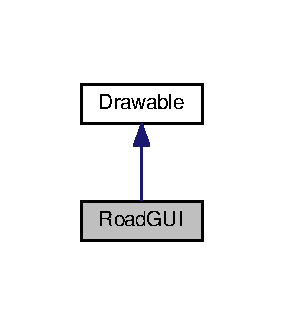
\includegraphics[width=136pt]{classRoadGUI__coll__graph}
\end{center}
\end{figure}
\subsection*{Public Member Functions}
\begin{DoxyCompactItemize}
\item 
\hyperlink{classRoadGUI_acfdd2c56d642c80612b54f6a0fa05cc5}{Road\-G\-U\-I} (\hyperlink{classPoint}{Point} begin, \hyperlink{classPoint}{Point} end, bool ghost=false)
\begin{DoxyCompactList}\small\item\em \hyperlink{classRoadGUI_acfdd2c56d642c80612b54f6a0fa05cc5}{Road\-G\-U\-I\-::\-Road\-G\-U\-I}. Constructor. \end{DoxyCompactList}\item 
\hyperlink{classRoadGUI_af093d97dcb41ce7d13d6ca37245ab5ac}{Road\-G\-U\-I} (\hyperlink{classPoint}{Point} point)
\begin{DoxyCompactList}\small\item\em \hyperlink{classRoadGUI_acfdd2c56d642c80612b54f6a0fa05cc5}{Road\-G\-U\-I\-::\-Road\-G\-U\-I}. Constructor. \end{DoxyCompactList}\item 
void \hyperlink{classRoadGUI_a7cff0e8608cff8223f41b4a266fcb4b2}{draw} (Q\-Painter \&) const override
\begin{DoxyCompactList}\small\item\em \hyperlink{classRoadGUI_a7cff0e8608cff8223f41b4a266fcb4b2}{Road\-G\-U\-I\-::draw}. \end{DoxyCompactList}\item 
\hypertarget{classRoadGUI_aa1e823a3c4afcc07fb64b9c984eddb50}{void {\bfseries set\-To} (unsigned int x, unsigned int y) override}\label{classRoadGUI_aa1e823a3c4afcc07fb64b9c984eddb50}

\item 
bool \hyperlink{classRoadGUI_a32b9692ed94d6efe1d194f7ba35af7c5}{intersects} (Q\-Rect \&rectangle) const override
\begin{DoxyCompactList}\small\item\em \hyperlink{classRoadGUI_a32b9692ed94d6efe1d194f7ba35af7c5}{Road\-G\-U\-I\-::intersects}. \end{DoxyCompactList}\item 
void \hyperlink{classRoadGUI_aad20fd36c29dedd57ed07cce3c391677}{set\-Rectangle} (\hyperlink{classPoint}{Point} first, \hyperlink{classPoint}{Point} second)
\begin{DoxyCompactList}\small\item\em \hyperlink{classRoadGUI_aad20fd36c29dedd57ed07cce3c391677}{Road\-G\-U\-I\-::set\-Rectangle}. \end{DoxyCompactList}\item 
void \hyperlink{classRoadGUI_a9ba81129f297df4ea1f0cc47e68a21f5}{set\-Rectangle} (\hyperlink{classPoint}{Point} point)
\begin{DoxyCompactList}\small\item\em \hyperlink{classRoadGUI_aad20fd36c29dedd57ed07cce3c391677}{Road\-G\-U\-I\-::set\-Rectangle}. \end{DoxyCompactList}\item 
void \hyperlink{classRoadGUI_a4c9c5617846bdcf4033bc36cdab72ea2}{draw\-Sidewalk} (Q\-Painter \&) const 
\begin{DoxyCompactList}\small\item\em \hyperlink{classRoadGUI_a4c9c5617846bdcf4033bc36cdab72ea2}{Road\-G\-U\-I\-::draw\-Sidewalk}. \end{DoxyCompactList}\item 
bool \hyperlink{classRoadGUI_a6d2d17128a1aa200bc312778761be70a}{is\-Vertical} () const 
\begin{DoxyCompactList}\small\item\em \hyperlink{classRoadGUI_a6d2d17128a1aa200bc312778761be70a}{Road\-G\-U\-I\-::is\-Vertical}. \end{DoxyCompactList}\item 
std\-::tuple$<$ \hyperlink{classPoint}{Point}, \hyperlink{classPoint}{Point} $>$ \hyperlink{classRoadGUI_a8fc09e0061ce1e02be7a17e27861abd3}{get\-Ends} () const 
\begin{DoxyCompactList}\small\item\em \hyperlink{classRoadGUI_a8fc09e0061ce1e02be7a17e27861abd3}{Road\-G\-U\-I\-::get\-Ends}. \end{DoxyCompactList}\end{DoxyCompactItemize}
\subsection*{Static Public Member Functions}
\begin{DoxyCompactItemize}
\item 
static void \hyperlink{classRoadGUI_ab990a1e8cba81b3da4dc4154239dcab4}{adjust\-Points} (\hyperlink{classPoint}{Point} \&first, \hyperlink{classPoint}{Point} \&second)
\begin{DoxyCompactList}\small\item\em \hyperlink{classRoadGUI_ab990a1e8cba81b3da4dc4154239dcab4}{Road\-G\-U\-I\-::adjust\-Points}. \end{DoxyCompactList}\end{DoxyCompactItemize}
\subsection*{Static Public Attributes}
\begin{DoxyCompactItemize}
\item 
static const int \hyperlink{classRoadGUI_a998dae57fd63610094da9e39f13c61c1}{P\-E\-N\-\_\-\-W\-I\-D\-T\-H} = 0
\item 
\hypertarget{classRoadGUI_ab9a0928afa237bd89691076633cf2991}{static const Qt\-::\-Pen\-Style {\bfseries P\-E\-N\-\_\-\-S\-T\-Y\-L\-E} = Qt\-::\-Solid\-Line}\label{classRoadGUI_ab9a0928afa237bd89691076633cf2991}

\item 
\hypertarget{classRoadGUI_a9ebf1722a441634ecb875611ac4a67f1}{static const Qt\-::\-Pen\-Cap\-Style {\bfseries P\-E\-N\-\_\-\-C\-A\-P} = Qt\-::\-Square\-Cap}\label{classRoadGUI_a9ebf1722a441634ecb875611ac4a67f1}

\item 
\hypertarget{classRoadGUI_aaa2a0fb2b5e6a0222428eb2fab48ea20}{static const Qt\-::\-Pen\-Join\-Style {\bfseries P\-E\-N\-\_\-\-J\-O\-I\-N} = Qt\-::\-Round\-Join}\label{classRoadGUI_aaa2a0fb2b5e6a0222428eb2fab48ea20}

\item 
\hypertarget{classRoadGUI_a2d69709533ad02ce74400b7354bc7b20}{static const Q\-Color {\bfseries P\-E\-N\-\_\-\-C\-O\-L\-O\-R} = Q\-Color(100, 100, 100, 0)}\label{classRoadGUI_a2d69709533ad02ce74400b7354bc7b20}

\item 
\hypertarget{classRoadGUI_afcae87f471384ff5ed4b9539b3e42e0d}{static const Q\-Color {\bfseries G\-H\-O\-S\-T\-\_\-\-P\-E\-N\-\_\-\-C\-O\-L\-O\-R} = Q\-Color(100, 100, 100, 0)}\label{classRoadGUI_afcae87f471384ff5ed4b9539b3e42e0d}

\item 
\hypertarget{classRoadGUI_aaad4b7b5899c833fe78c60a7583ccbfc}{static const Q\-Pen {\bfseries P\-E\-N}}\label{classRoadGUI_aaad4b7b5899c833fe78c60a7583ccbfc}

\item 
\hypertarget{classRoadGUI_a967cb8f74565726887990dc748fca996}{static const Q\-Pen {\bfseries G\-H\-O\-S\-T\-\_\-\-P\-E\-N}}\label{classRoadGUI_a967cb8f74565726887990dc748fca996}

\item 
\hypertarget{classRoadGUI_a53dc510ed73ce2310670ba56a60387d9}{static const Qt\-::\-Brush\-Style {\bfseries B\-R\-U\-S\-H\-\_\-\-S\-T\-Y\-L\-E} = Qt\-::\-Solid\-Pattern}\label{classRoadGUI_a53dc510ed73ce2310670ba56a60387d9}

\item 
\hypertarget{classRoadGUI_aab9d1e45204227a7deb5be52f8f2a698}{static const Q\-Color {\bfseries B\-R\-U\-S\-H\-\_\-\-C\-O\-L\-O\-R} = Q\-Color(72, 72, 59)}\label{classRoadGUI_aab9d1e45204227a7deb5be52f8f2a698}

\item 
\hypertarget{classRoadGUI_af38f8106a9e1b0f7dc60fe6719b79034}{static const Q\-Color {\bfseries G\-H\-O\-S\-T\-\_\-\-B\-R\-U\-S\-H\-\_\-\-C\-O\-L\-O\-R} = Q\-Color(72, 72, 59, 127)}\label{classRoadGUI_af38f8106a9e1b0f7dc60fe6719b79034}

\item 
\hypertarget{classRoadGUI_a1bac52c458cdf4ea063345186bd59a88}{static const Q\-Brush {\bfseries B\-R\-U\-S\-H}}\label{classRoadGUI_a1bac52c458cdf4ea063345186bd59a88}

\item 
\hypertarget{classRoadGUI_a0c717e32cd1bea3c52a840f3915c7785}{static const Q\-Brush {\bfseries G\-H\-O\-S\-T\-\_\-\-B\-R\-U\-S\-H}}\label{classRoadGUI_a0c717e32cd1bea3c52a840f3915c7785}

\item 
\hypertarget{classRoadGUI_aaea72d54185d2dd5226f71ffe12b17a8}{static const Q\-Color {\bfseries S\-I\-D\-E\-W\-A\-L\-K\-\_\-\-B\-R\-U\-S\-H\-\_\-\-C\-O\-L\-O\-R} = Q\-Color(155, 155, 132)}\label{classRoadGUI_aaea72d54185d2dd5226f71ffe12b17a8}

\item 
\hypertarget{classRoadGUI_a1a0d50da26147c147851f0ce7e4becde}{static const Q\-Brush {\bfseries S\-I\-D\-E\-W\-A\-L\-K\-\_\-\-B\-R\-U\-S\-H}}\label{classRoadGUI_a1a0d50da26147c147851f0ce7e4becde}

\item 
\hypertarget{classRoadGUI_a2ebb95704c366ffb0bd8d2dcd0380b27}{static const unsigned int {\bfseries S\-I\-D\-E\-W\-A\-L\-K\-\_\-\-W\-I\-D\-T\-H} = 8}\label{classRoadGUI_a2ebb95704c366ffb0bd8d2dcd0380b27}

\end{DoxyCompactItemize}


\subsection{Detailed Description}
The \hyperlink{classRoadGUI}{Road\-G\-U\-I} class. Class holds info about look of roads in G\-U\-I. 

Class holds information necessary to draw road object on screen. It implements virtual function draw. It additionally has function draw\-Sidewalk, so sidewalks can be drawn below all roads. Without caling this function, sidewalks won't appear. It also holds all information about how roads and sidewalks are supposed to look. \begin{DoxyAuthor}{Author}
Pawel Rybak 
\end{DoxyAuthor}


\subsection{Constructor \& Destructor Documentation}
\hypertarget{classRoadGUI_acfdd2c56d642c80612b54f6a0fa05cc5}{\index{Road\-G\-U\-I@{Road\-G\-U\-I}!Road\-G\-U\-I@{Road\-G\-U\-I}}
\index{Road\-G\-U\-I@{Road\-G\-U\-I}!RoadGUI@{Road\-G\-U\-I}}
\subsubsection[{Road\-G\-U\-I}]{\setlength{\rightskip}{0pt plus 5cm}Road\-G\-U\-I\-::\-Road\-G\-U\-I (
\begin{DoxyParamCaption}
\item[{{\bf Point}}]{first\-Point, }
\item[{{\bf Point}}]{second\-Point, }
\item[{bool}]{ghost = {\ttfamily false}}
\end{DoxyParamCaption}
)}}\label{classRoadGUI_acfdd2c56d642c80612b54f6a0fa05cc5}


\hyperlink{classRoadGUI_acfdd2c56d642c80612b54f6a0fa05cc5}{Road\-G\-U\-I\-::\-Road\-G\-U\-I}. Constructor. 


\begin{DoxyParams}{Parameters}
{\em first\-Point} & -\/ One end of the road. \\
\hline
{\em second\-Point} & -\/ Other end of the road. \\
\hline
{\em ghost} & -\/ Bool flag tells whether object is ghost object.\\
\hline
\end{DoxyParams}
Constructs object based on two points given as arguments. Line created by points doesn't have to be horizontal or vertical. Road is going to be made horizontal or vertical based on difference between points (dx $>$ dy). \hypertarget{classRoadGUI_af093d97dcb41ce7d13d6ca37245ab5ac}{\index{Road\-G\-U\-I@{Road\-G\-U\-I}!Road\-G\-U\-I@{Road\-G\-U\-I}}
\index{Road\-G\-U\-I@{Road\-G\-U\-I}!RoadGUI@{Road\-G\-U\-I}}
\subsubsection[{Road\-G\-U\-I}]{\setlength{\rightskip}{0pt plus 5cm}Road\-G\-U\-I\-::\-Road\-G\-U\-I (
\begin{DoxyParamCaption}
\item[{{\bf Point}}]{point}
\end{DoxyParamCaption}
)}}\label{classRoadGUI_af093d97dcb41ce7d13d6ca37245ab5ac}


\hyperlink{classRoadGUI_acfdd2c56d642c80612b54f6a0fa05cc5}{Road\-G\-U\-I\-::\-Road\-G\-U\-I}. Constructor. 


\begin{DoxyParams}{Parameters}
{\em point} & -\/ \hyperlink{classPoint}{Point}.\\
\hline
\end{DoxyParams}
Creates temporary ghost road being just a square. 

\subsection{Member Function Documentation}
\hypertarget{classRoadGUI_ab990a1e8cba81b3da4dc4154239dcab4}{\index{Road\-G\-U\-I@{Road\-G\-U\-I}!adjust\-Points@{adjust\-Points}}
\index{adjust\-Points@{adjust\-Points}!RoadGUI@{Road\-G\-U\-I}}
\subsubsection[{adjust\-Points}]{\setlength{\rightskip}{0pt plus 5cm}void Road\-G\-U\-I\-::adjust\-Points (
\begin{DoxyParamCaption}
\item[{{\bf Point} \&}]{first, }
\item[{{\bf Point} \&}]{second}
\end{DoxyParamCaption}
)\hspace{0.3cm}{\ttfamily [static]}}}\label{classRoadGUI_ab990a1e8cba81b3da4dc4154239dcab4}


\hyperlink{classRoadGUI_ab990a1e8cba81b3da4dc4154239dcab4}{Road\-G\-U\-I\-::adjust\-Points}. 


\begin{DoxyParams}{Parameters}
{\em first} & -\/ Reference to first point. \\
\hline
{\em second} & -\/ Reference to second point.\\
\hline
\end{DoxyParams}
Function takes reference to two points and sets them in line parallel to horizontal or vertical, based on difference between these points (dx $>$ dy). \hypertarget{classRoadGUI_a7cff0e8608cff8223f41b4a266fcb4b2}{\index{Road\-G\-U\-I@{Road\-G\-U\-I}!draw@{draw}}
\index{draw@{draw}!RoadGUI@{Road\-G\-U\-I}}
\subsubsection[{draw}]{\setlength{\rightskip}{0pt plus 5cm}void Road\-G\-U\-I\-::draw (
\begin{DoxyParamCaption}
\item[{Q\-Painter \&}]{painter}
\end{DoxyParamCaption}
) const\hspace{0.3cm}{\ttfamily [override]}, {\ttfamily [virtual]}}}\label{classRoadGUI_a7cff0e8608cff8223f41b4a266fcb4b2}


\hyperlink{classRoadGUI_a7cff0e8608cff8223f41b4a266fcb4b2}{Road\-G\-U\-I\-::draw}. 


\begin{DoxyParams}{Parameters}
{\em painter} & -\/ Reference to painter object.\\
\hline
\end{DoxyParams}
Function draws object using painter given as an argument. It uses brushes, and pens defined in object, and base its choice on whether it is ghost object or not. 

Implements \hyperlink{classDrawable}{Drawable}.

\hypertarget{classRoadGUI_a4c9c5617846bdcf4033bc36cdab72ea2}{\index{Road\-G\-U\-I@{Road\-G\-U\-I}!draw\-Sidewalk@{draw\-Sidewalk}}
\index{draw\-Sidewalk@{draw\-Sidewalk}!RoadGUI@{Road\-G\-U\-I}}
\subsubsection[{draw\-Sidewalk}]{\setlength{\rightskip}{0pt plus 5cm}void Road\-G\-U\-I\-::draw\-Sidewalk (
\begin{DoxyParamCaption}
\item[{Q\-Painter \&}]{painter}
\end{DoxyParamCaption}
) const}}\label{classRoadGUI_a4c9c5617846bdcf4033bc36cdab72ea2}


\hyperlink{classRoadGUI_a4c9c5617846bdcf4033bc36cdab72ea2}{Road\-G\-U\-I\-::draw\-Sidewalk}. 


\begin{DoxyParams}{Parameters}
{\em painter} & -\/ Reference to painter object.\\
\hline
\end{DoxyParams}
Function draws sidewalk using painter given as an argument. It uses brushes, and pens defined in object. Ghost roads doesnt have sidewalks. \hypertarget{classRoadGUI_a8fc09e0061ce1e02be7a17e27861abd3}{\index{Road\-G\-U\-I@{Road\-G\-U\-I}!get\-Ends@{get\-Ends}}
\index{get\-Ends@{get\-Ends}!RoadGUI@{Road\-G\-U\-I}}
\subsubsection[{get\-Ends}]{\setlength{\rightskip}{0pt plus 5cm}std\-::tuple$<$ {\bf Point}, {\bf Point} $>$ Road\-G\-U\-I\-::get\-Ends (
\begin{DoxyParamCaption}
{}
\end{DoxyParamCaption}
) const}}\label{classRoadGUI_a8fc09e0061ce1e02be7a17e27861abd3}


\hyperlink{classRoadGUI_a8fc09e0061ce1e02be7a17e27861abd3}{Road\-G\-U\-I\-::get\-Ends}. 

\begin{DoxyReturn}{Returns}
Returns tuple with two ends of road. 
\end{DoxyReturn}
\hypertarget{classRoadGUI_a32b9692ed94d6efe1d194f7ba35af7c5}{\index{Road\-G\-U\-I@{Road\-G\-U\-I}!intersects@{intersects}}
\index{intersects@{intersects}!RoadGUI@{Road\-G\-U\-I}}
\subsubsection[{intersects}]{\setlength{\rightskip}{0pt plus 5cm}bool Road\-G\-U\-I\-::intersects (
\begin{DoxyParamCaption}
\item[{Q\-Rect \&}]{rectangle}
\end{DoxyParamCaption}
) const\hspace{0.3cm}{\ttfamily [override]}, {\ttfamily [virtual]}}}\label{classRoadGUI_a32b9692ed94d6efe1d194f7ba35af7c5}


\hyperlink{classRoadGUI_a32b9692ed94d6efe1d194f7ba35af7c5}{Road\-G\-U\-I\-::intersects}. 


\begin{DoxyParams}{Parameters}
{\em rectangle} & -\/ Q\-Rect object that is being checked for intersection. \\
\hline
\end{DoxyParams}
\begin{DoxyReturn}{Returns}
Bool value whether rectangles intersects.
\end{DoxyReturn}
Function checks whether current road's (not including sight range) rectangle intersects rectangle given as argument and returns bool value. 

Implements \hyperlink{classDrawable}{Drawable}.

\hypertarget{classRoadGUI_a6d2d17128a1aa200bc312778761be70a}{\index{Road\-G\-U\-I@{Road\-G\-U\-I}!is\-Vertical@{is\-Vertical}}
\index{is\-Vertical@{is\-Vertical}!RoadGUI@{Road\-G\-U\-I}}
\subsubsection[{is\-Vertical}]{\setlength{\rightskip}{0pt plus 5cm}bool Road\-G\-U\-I\-::is\-Vertical (
\begin{DoxyParamCaption}
{}
\end{DoxyParamCaption}
) const}}\label{classRoadGUI_a6d2d17128a1aa200bc312778761be70a}


\hyperlink{classRoadGUI_a6d2d17128a1aa200bc312778761be70a}{Road\-G\-U\-I\-::is\-Vertical}. 

\begin{DoxyReturn}{Returns}
Returns flag whether function is vertical or not 
\end{DoxyReturn}
\hypertarget{classRoadGUI_aad20fd36c29dedd57ed07cce3c391677}{\index{Road\-G\-U\-I@{Road\-G\-U\-I}!set\-Rectangle@{set\-Rectangle}}
\index{set\-Rectangle@{set\-Rectangle}!RoadGUI@{Road\-G\-U\-I}}
\subsubsection[{set\-Rectangle}]{\setlength{\rightskip}{0pt plus 5cm}void Road\-G\-U\-I\-::set\-Rectangle (
\begin{DoxyParamCaption}
\item[{{\bf Point}}]{first, }
\item[{{\bf Point}}]{second}
\end{DoxyParamCaption}
)}}\label{classRoadGUI_aad20fd36c29dedd57ed07cce3c391677}


\hyperlink{classRoadGUI_aad20fd36c29dedd57ed07cce3c391677}{Road\-G\-U\-I\-::set\-Rectangle}. 


\begin{DoxyParams}{Parameters}
{\em first} & -\/ One end of the road. \\
\hline
{\em second} & -\/ Other end of the road.\\
\hline
\end{DoxyParams}
Function sets road to be between two given points. Line created by points doesn't have to be horizontal or vertical. Road is going to be made horizontal or vertical based on difference between points (dx $>$ dy). \hypertarget{classRoadGUI_a9ba81129f297df4ea1f0cc47e68a21f5}{\index{Road\-G\-U\-I@{Road\-G\-U\-I}!set\-Rectangle@{set\-Rectangle}}
\index{set\-Rectangle@{set\-Rectangle}!RoadGUI@{Road\-G\-U\-I}}
\subsubsection[{set\-Rectangle}]{\setlength{\rightskip}{0pt plus 5cm}void Road\-G\-U\-I\-::set\-Rectangle (
\begin{DoxyParamCaption}
\item[{{\bf Point}}]{point}
\end{DoxyParamCaption}
)}}\label{classRoadGUI_a9ba81129f297df4ea1f0cc47e68a21f5}


\hyperlink{classRoadGUI_aad20fd36c29dedd57ed07cce3c391677}{Road\-G\-U\-I\-::set\-Rectangle}. 


\begin{DoxyParams}{Parameters}
{\em point} & -\/ \hyperlink{classPoint}{Point} of new road.\\
\hline
\end{DoxyParams}
Function sets temporary ghost road in point given as argument. 

\subsection{Member Data Documentation}
\hypertarget{classRoadGUI_a998dae57fd63610094da9e39f13c61c1}{\index{Road\-G\-U\-I@{Road\-G\-U\-I}!P\-E\-N\-\_\-\-W\-I\-D\-T\-H@{P\-E\-N\-\_\-\-W\-I\-D\-T\-H}}
\index{P\-E\-N\-\_\-\-W\-I\-D\-T\-H@{P\-E\-N\-\_\-\-W\-I\-D\-T\-H}!RoadGUI@{Road\-G\-U\-I}}
\subsubsection[{P\-E\-N\-\_\-\-W\-I\-D\-T\-H}]{\setlength{\rightskip}{0pt plus 5cm}const int Road\-G\-U\-I\-::\-P\-E\-N\-\_\-\-W\-I\-D\-T\-H = 0\hspace{0.3cm}{\ttfamily [static]}}}\label{classRoadGUI_a998dae57fd63610094da9e39f13c61c1}
P\-R\-O\-P\-E\-R\-T\-I\-E\-S

P\-R\-O\-P\-E\-R\-T\-I\-E\-S I\-N\-I\-T\-I\-A\-L\-I\-Z\-E 

The documentation for this class was generated from the following files\-:\begin{DoxyCompactItemize}
\item 
/home/aleksander/\-C\-Lion\-Projects/\-Zpr/src/\-G\-U\-I/roadgui.\-h\item 
/home/aleksander/\-C\-Lion\-Projects/\-Zpr/src/\-G\-U\-I/roadgui.\-cpp\end{DoxyCompactItemize}

\hypertarget{classRoute}{\section{Route Class Reference}
\label{classRoute}\index{Route@{Route}}
}


{\ttfamily \#include $<$Route.\-h$>$}



Inheritance diagram for Route\-:
\nopagebreak
\begin{figure}[H]
\begin{center}
\leavevmode
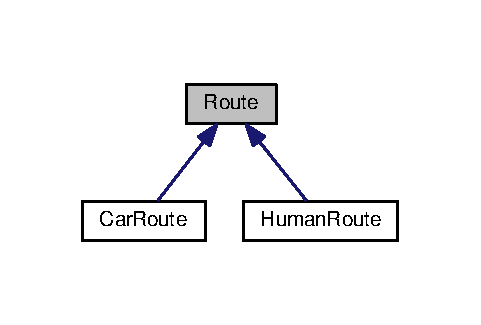
\includegraphics[width=231pt]{classRoute__inherit__graph}
\end{center}
\end{figure}
\subsection*{Public Member Functions}
\begin{DoxyCompactItemize}
\item 
\hyperlink{classRouteVector}{Route\-Vector} \hyperlink{classRoute_aade7196ddcba6bc6191495992a3abbbe}{get\-Route\-Vector} (const \hyperlink{classPoint}{Point} \&point) const 
\item 
int \hyperlink{classRoute_a637b4390cd5b98be93d7481232bf173d}{get\-Distance} (const \hyperlink{classPoint}{Point} \&point) const 
\item 
virtual bool \hyperlink{classRoute_a27bb16170420801b5c191e9aea0134f1}{next\-Point} ()=0
\item 
virtual bool \hyperlink{classRoute_a0e1d104b56c768549f1b4fe4b575a6f5}{is\-End} ()=0
\end{DoxyCompactItemize}


\subsection{Detailed Description}
This class represents route(\-G\-P\-S). \begin{DoxyAuthor}{Author}
Aleksander Brzozowski 
\end{DoxyAuthor}


\subsection{Member Function Documentation}
\hypertarget{classRoute_a637b4390cd5b98be93d7481232bf173d}{\index{Route@{Route}!get\-Distance@{get\-Distance}}
\index{get\-Distance@{get\-Distance}!Route@{Route}}
\subsubsection[{get\-Distance}]{\setlength{\rightskip}{0pt plus 5cm}int Route\-::get\-Distance (
\begin{DoxyParamCaption}
\item[{const {\bf Point} \&}]{point}
\end{DoxyParamCaption}
) const}}\label{classRoute_a637b4390cd5b98be93d7481232bf173d}
Computes distance between point and actual point of \hyperlink{classRoute}{Route}. 
\begin{DoxyParams}{Parameters}
{\em point} & \hyperlink{classPoint}{Point} to which distance will be computed \\
\hline
\end{DoxyParams}
\begin{DoxyReturn}{Returns}
Distance between point and actual point of \hyperlink{classRoute}{Route} 
\end{DoxyReturn}
\hypertarget{classRoute_aade7196ddcba6bc6191495992a3abbbe}{\index{Route@{Route}!get\-Route\-Vector@{get\-Route\-Vector}}
\index{get\-Route\-Vector@{get\-Route\-Vector}!Route@{Route}}
\subsubsection[{get\-Route\-Vector}]{\setlength{\rightskip}{0pt plus 5cm}{\bf Route\-Vector} Route\-::get\-Route\-Vector (
\begin{DoxyParamCaption}
\item[{const {\bf Point} \&}]{point}
\end{DoxyParamCaption}
) const}}\label{classRoute_aade7196ddcba6bc6191495992a3abbbe}
Computes vector between actual point of \hyperlink{classRoute}{Route} and passed point. 
\begin{DoxyParams}{Parameters}
{\em point} & \hyperlink{classPoint}{Point} to which vector will be computed \\
\hline
\end{DoxyParams}
\begin{DoxyReturn}{Returns}
Vector to fallow 
\end{DoxyReturn}
\hypertarget{classRoute_a0e1d104b56c768549f1b4fe4b575a6f5}{\index{Route@{Route}!is\-End@{is\-End}}
\index{is\-End@{is\-End}!Route@{Route}}
\subsubsection[{is\-End}]{\setlength{\rightskip}{0pt plus 5cm}virtual bool Route\-::is\-End (
\begin{DoxyParamCaption}
{}
\end{DoxyParamCaption}
)\hspace{0.3cm}{\ttfamily [pure virtual]}}}\label{classRoute_a0e1d104b56c768549f1b4fe4b575a6f5}
Checks is it end of \hyperlink{classRoute}{Route}. \begin{DoxyReturn}{Returns}
is end of \hyperlink{classRoute}{Route} 
\end{DoxyReturn}


Implemented in \hyperlink{classCarRoute_a4d8589aeb5b9accd189756dda8b618c6}{Car\-Route}, and \hyperlink{classHumanRoute_aee549e955710a5217ba763d2320fb0ea}{Human\-Route}.

\hypertarget{classRoute_a27bb16170420801b5c191e9aea0134f1}{\index{Route@{Route}!next\-Point@{next\-Point}}
\index{next\-Point@{next\-Point}!Route@{Route}}
\subsubsection[{next\-Point}]{\setlength{\rightskip}{0pt plus 5cm}virtual bool Route\-::next\-Point (
\begin{DoxyParamCaption}
{}
\end{DoxyParamCaption}
)\hspace{0.3cm}{\ttfamily [pure virtual]}}}\label{classRoute_a27bb16170420801b5c191e9aea0134f1}
Switches to the next point of route. \begin{DoxyReturn}{Returns}
Is next point of route 
\end{DoxyReturn}


Implemented in \hyperlink{classCarRoute_a48a60e9054bcb3b775f4a56b50c0d79d}{Car\-Route}, and \hyperlink{classHumanRoute_a89c5021044b130a2928eb933111bf390}{Human\-Route}.



The documentation for this class was generated from the following files\-:\begin{DoxyCompactItemize}
\item 
/home/aleksander/\-C\-Lion\-Projects/\-Zpr/src/Route.\-h\item 
/home/aleksander/\-C\-Lion\-Projects/\-Zpr/src/Route.\-cpp\end{DoxyCompactItemize}

\hypertarget{classRouteVector}{\section{Route\-Vector Class Reference}
\label{classRouteVector}\index{Route\-Vector@{Route\-Vector}}
}


{\ttfamily \#include $<$Route\-Vector.\-h$>$}

\subsection*{Public Member Functions}
\begin{DoxyCompactItemize}
\item 
\hyperlink{classRouteVector_a08a0cdeb28a7f4de7d4be94da30debd7}{Route\-Vector} (const \hyperlink{classPoint}{Point} \&begin, const \hyperlink{classPoint}{Point} \&end)
\item 
\hyperlink{classRouteVector_ac3796e8702b7dba67eac66bfc1cb6b3b}{Route\-Vector} ()
\item 
\hyperlink{classRouteVector_a9dc4fc2b73469b6a9261036877262722}{Route\-Vector} (int x, int y)
\item 
\hypertarget{classRouteVector_a8971cddddcfa0be5fd1430ac516a69f3}{bool {\bfseries operator==} (const \hyperlink{classRouteVector}{Route\-Vector} \&rhs) const }\label{classRouteVector_a8971cddddcfa0be5fd1430ac516a69f3}

\item 
\hypertarget{classRouteVector_acc459698bbd65ed871c4b5a13466f11f}{bool {\bfseries operator!=} (const \hyperlink{classRouteVector}{Route\-Vector} \&rhs) const }\label{classRouteVector_acc459698bbd65ed871c4b5a13466f11f}

\item 
\hypertarget{classRouteVector_adf1ea492130b9f73ee1f45f4dc80b092}{int {\bfseries get\-X} () const }\label{classRouteVector_adf1ea492130b9f73ee1f45f4dc80b092}

\item 
\hypertarget{classRouteVector_a077707d02a8a63d9cdd9783e16dc8097}{int {\bfseries get\-Y} () const }\label{classRouteVector_a077707d02a8a63d9cdd9783e16dc8097}

\end{DoxyCompactItemize}


\subsection{Detailed Description}
Represents vector. \begin{DoxyAuthor}{Author}
Aleksander Brzozowski 
\end{DoxyAuthor}


\subsection{Constructor \& Destructor Documentation}
\hypertarget{classRouteVector_a08a0cdeb28a7f4de7d4be94da30debd7}{\index{Route\-Vector@{Route\-Vector}!Route\-Vector@{Route\-Vector}}
\index{Route\-Vector@{Route\-Vector}!RouteVector@{Route\-Vector}}
\subsubsection[{Route\-Vector}]{\setlength{\rightskip}{0pt plus 5cm}Route\-Vector\-::\-Route\-Vector (
\begin{DoxyParamCaption}
\item[{const {\bf Point} \&}]{begin, }
\item[{const {\bf Point} \&}]{end}
\end{DoxyParamCaption}
)}}\label{classRouteVector_a08a0cdeb28a7f4de7d4be94da30debd7}
Constructs vector between two points that have same x or y. Normalizes vector to 1. Possible vectors are\-: \mbox{[}-\/1, 0\mbox{]}, \mbox{[}1, 0\mbox{]}, \mbox{[}0, -\/1\mbox{]}, \mbox{[}0, 1\mbox{]}, \mbox{[}0, 0\mbox{]}. 
\begin{DoxyExceptions}{Exceptions}
{\em std\-::invalid\-\_\-argument} & When points don't have same x or y \\
\hline
\end{DoxyExceptions}

\begin{DoxyParams}{Parameters}
{\em begin} & First point \\
\hline
{\em end} & Second point \\
\hline
\end{DoxyParams}
\hypertarget{classRouteVector_ac3796e8702b7dba67eac66bfc1cb6b3b}{\index{Route\-Vector@{Route\-Vector}!Route\-Vector@{Route\-Vector}}
\index{Route\-Vector@{Route\-Vector}!RouteVector@{Route\-Vector}}
\subsubsection[{Route\-Vector}]{\setlength{\rightskip}{0pt plus 5cm}Route\-Vector\-::\-Route\-Vector (
\begin{DoxyParamCaption}
{}
\end{DoxyParamCaption}
)}}\label{classRouteVector_ac3796e8702b7dba67eac66bfc1cb6b3b}
Constructs \mbox{[}0, 0\mbox{]} vector. \hypertarget{classRouteVector_a9dc4fc2b73469b6a9261036877262722}{\index{Route\-Vector@{Route\-Vector}!Route\-Vector@{Route\-Vector}}
\index{Route\-Vector@{Route\-Vector}!RouteVector@{Route\-Vector}}
\subsubsection[{Route\-Vector}]{\setlength{\rightskip}{0pt plus 5cm}Route\-Vector\-::\-Route\-Vector (
\begin{DoxyParamCaption}
\item[{int}]{x, }
\item[{int}]{y}
\end{DoxyParamCaption}
)}}\label{classRouteVector_a9dc4fc2b73469b6a9261036877262722}
Constructs vector using passed x and y \mbox{[}x, y\mbox{]}. 
\begin{DoxyParams}{Parameters}
{\em x} & Vector's x \\
\hline
{\em y} & Vector's y \\
\hline
\end{DoxyParams}


The documentation for this class was generated from the following files\-:\begin{DoxyCompactItemize}
\item 
/home/aleksander/\-C\-Lion\-Projects/\-Zpr/src/Route\-Vector.\-h\item 
/home/aleksander/\-C\-Lion\-Projects/\-Zpr/src/Route\-Vector.\-cpp\end{DoxyCompactItemize}

\hypertarget{classUi__MainWindow}{\section{Ui\-\_\-\-Main\-Window Class Reference}
\label{classUi__MainWindow}\index{Ui\-\_\-\-Main\-Window@{Ui\-\_\-\-Main\-Window}}
}


Inheritance diagram for Ui\-\_\-\-Main\-Window\-:
\nopagebreak
\begin{figure}[H]
\begin{center}
\leavevmode
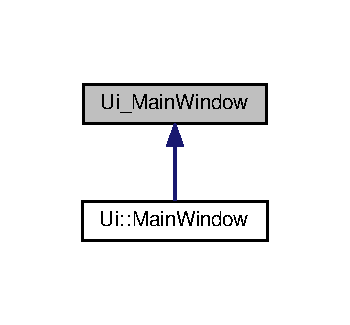
\includegraphics[width=168pt]{classUi__MainWindow__inherit__graph}
\end{center}
\end{figure}
\subsection*{Public Member Functions}
\begin{DoxyCompactItemize}
\item 
\hypertarget{classUi__MainWindow_acf4a0872c4c77d8f43a2ec66ed849b58}{void {\bfseries setup\-Ui} (Q\-Main\-Window $\ast$\hyperlink{classMainWindow}{Main\-Window})}\label{classUi__MainWindow_acf4a0872c4c77d8f43a2ec66ed849b58}

\item 
\hypertarget{classUi__MainWindow_a097dd160c3534a204904cb374412c618}{void {\bfseries retranslate\-Ui} (Q\-Main\-Window $\ast$\hyperlink{classMainWindow}{Main\-Window})}\label{classUi__MainWindow_a097dd160c3534a204904cb374412c618}

\end{DoxyCompactItemize}
\subsection*{Public Attributes}
\begin{DoxyCompactItemize}
\item 
\hypertarget{classUi__MainWindow_a30075506c2116c3ed4ff25e07ae75f81}{Q\-Widget $\ast$ {\bfseries central\-Widget}}\label{classUi__MainWindow_a30075506c2116c3ed4ff25e07ae75f81}

\item 
\hypertarget{classUi__MainWindow_a2be1c24ec9adfca18e1dcc951931457f}{Q\-Menu\-Bar $\ast$ {\bfseries menu\-Bar}}\label{classUi__MainWindow_a2be1c24ec9adfca18e1dcc951931457f}

\item 
\hypertarget{classUi__MainWindow_a50fa481337604bcc8bf68de18ab16ecd}{Q\-Status\-Bar $\ast$ {\bfseries status\-Bar}}\label{classUi__MainWindow_a50fa481337604bcc8bf68de18ab16ecd}

\end{DoxyCompactItemize}


The documentation for this class was generated from the following file\-:\begin{DoxyCompactItemize}
\item 
/home/aleksander/\-C\-Lion\-Projects/\-Zpr/src/\-G\-U\-I/ui\-\_\-mainwindow.\-h\end{DoxyCompactItemize}

\chapter{File Documentation}
\hypertarget{Cross_8cpp}{\section{/home/aleksander/\-C\-Lion\-Projects/\-Zpr/src/\-Cross.cpp File Reference}
\label{Cross_8cpp}\index{/home/aleksander/\-C\-Lion\-Projects/\-Zpr/src/\-Cross.\-cpp@{/home/aleksander/\-C\-Lion\-Projects/\-Zpr/src/\-Cross.\-cpp}}
}


\hyperlink{classCross}{Cross} class methods implementation.  


{\ttfamily \#include $<$stdexcept$>$}\\*
{\ttfamily \#include \char`\"{}Cross.\-h\char`\"{}}\\*
Include dependency graph for Cross.\-cpp\-:
\nopagebreak
\begin{figure}[H]
\begin{center}
\leavevmode
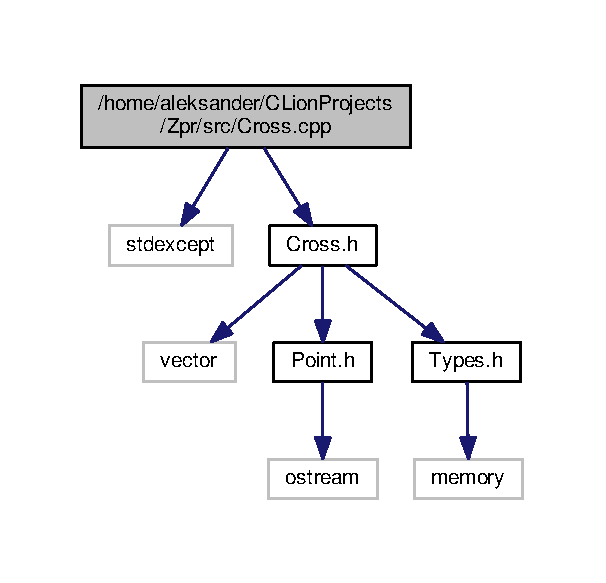
\includegraphics[width=291pt]{Cross_8cpp__incl}
\end{center}
\end{figure}


\subsection{Detailed Description}
\hyperlink{classCross}{Cross} class methods implementation. Piotr\-Kuc (\href{mailto:piotr.kuc29@gmail.com}{\tt piotr.\-kuc29@gmail.\-com}) \begin{DoxyDate}{Date}
November, 2017 
\end{DoxyDate}

\hypertarget{Cross_8h}{\section{/home/aleksander/\-C\-Lion\-Projects/\-Zpr/src/\-Cross.h File Reference}
\label{Cross_8h}\index{/home/aleksander/\-C\-Lion\-Projects/\-Zpr/src/\-Cross.\-h@{/home/aleksander/\-C\-Lion\-Projects/\-Zpr/src/\-Cross.\-h}}
}


\hyperlink{classCross}{Cross} class methods declaration.  


{\ttfamily \#include $<$vector$>$}\\*
{\ttfamily \#include \char`\"{}Point.\-h\char`\"{}}\\*
{\ttfamily \#include \char`\"{}Types.\-h\char`\"{}}\\*
Include dependency graph for Cross.\-h\-:
\nopagebreak
\begin{figure}[H]
\begin{center}
\leavevmode
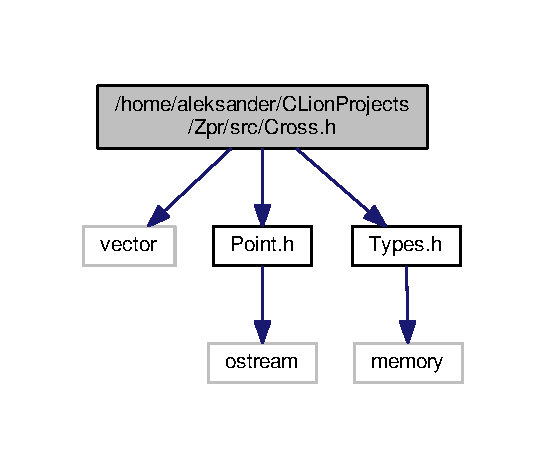
\includegraphics[width=262pt]{Cross_8h__incl}
\end{center}
\end{figure}
This graph shows which files directly or indirectly include this file\-:
\nopagebreak
\begin{figure}[H]
\begin{center}
\leavevmode
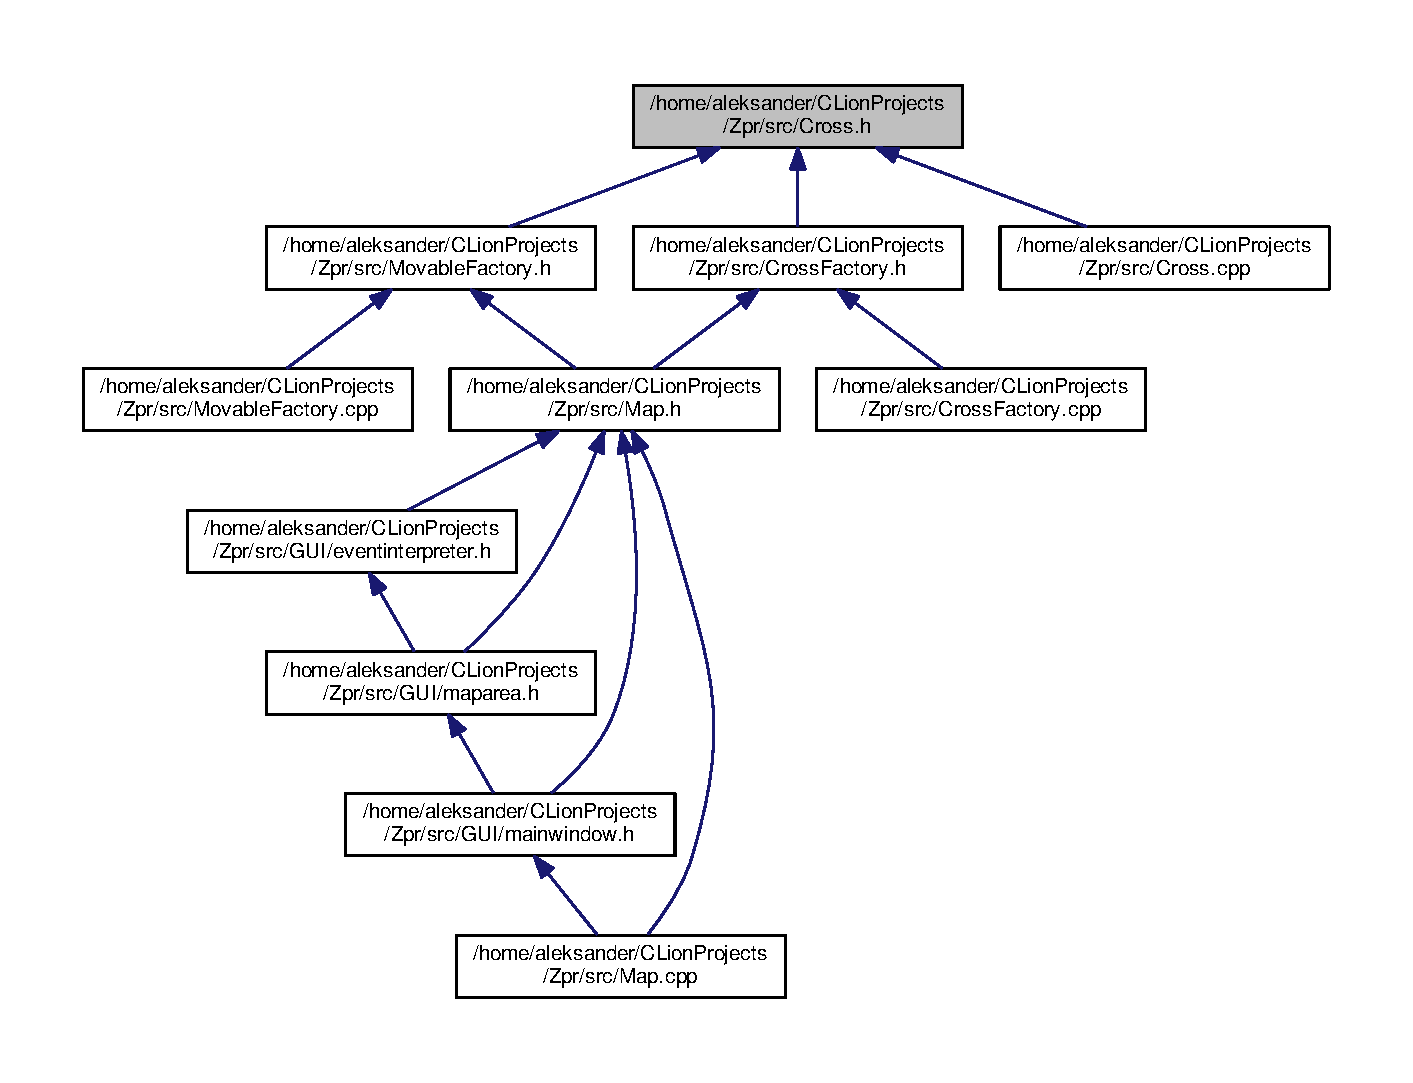
\includegraphics[width=350pt]{Cross_8h__dep__incl}
\end{center}
\end{figure}
\subsection*{Classes}
\begin{DoxyCompactItemize}
\item 
class \hyperlink{classCross}{Cross}
\begin{DoxyCompactList}\small\item\em \hyperlink{classCross}{Cross} represents vertices in the graph that describes map. \end{DoxyCompactList}\end{DoxyCompactItemize}


\subsection{Detailed Description}
\hyperlink{classCross}{Cross} class methods declaration. Piotr\-Kuc (\href{mailto:piotr.kuc29@gmail.com}{\tt piotr.\-kuc29@gmail.\-com}) \begin{DoxyDate}{Date}
November, 2017 
\end{DoxyDate}

\hypertarget{CrossFactory_8cpp}{\section{/home/aleksander/\-C\-Lion\-Projects/\-Zpr/src/\-Cross\-Factory.cpp File Reference}
\label{CrossFactory_8cpp}\index{/home/aleksander/\-C\-Lion\-Projects/\-Zpr/src/\-Cross\-Factory.\-cpp@{/home/aleksander/\-C\-Lion\-Projects/\-Zpr/src/\-Cross\-Factory.\-cpp}}
}


\hyperlink{classCrossFactory}{Cross\-Factory} class methods implementation.  


{\ttfamily \#include \char`\"{}Cross\-Factory.\-h\char`\"{}}\\*
Include dependency graph for Cross\-Factory.\-cpp\-:
\nopagebreak
\begin{figure}[H]
\begin{center}
\leavevmode
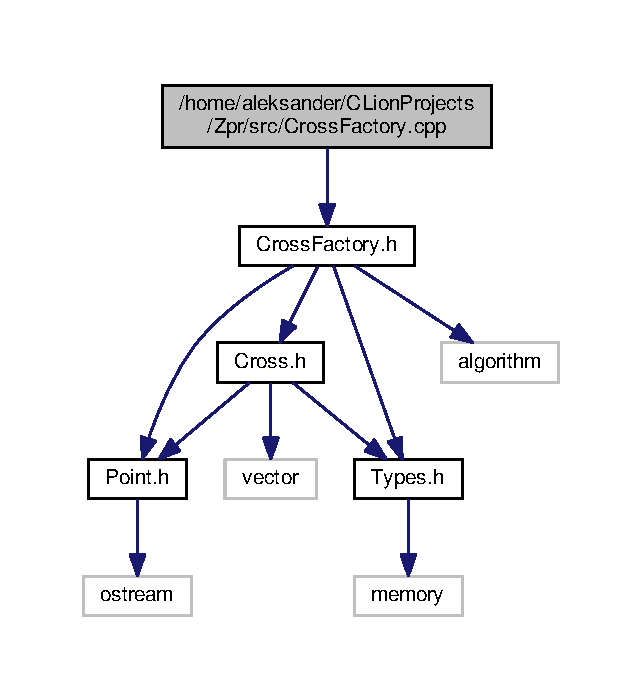
\includegraphics[width=308pt]{CrossFactory_8cpp__incl}
\end{center}
\end{figure}


\subsection{Detailed Description}
\hyperlink{classCrossFactory}{Cross\-Factory} class methods implementation. Piotr\-Kuc (\href{mailto:piotr.kuc29@gmail.com}{\tt piotr.\-kuc29@gmail.\-com}) \begin{DoxyDate}{Date}
December, 2017 
\end{DoxyDate}

\hypertarget{CrossFactory_8h}{\section{/home/aleksander/\-C\-Lion\-Projects/\-Zpr/src/\-Cross\-Factory.h File Reference}
\label{CrossFactory_8h}\index{/home/aleksander/\-C\-Lion\-Projects/\-Zpr/src/\-Cross\-Factory.\-h@{/home/aleksander/\-C\-Lion\-Projects/\-Zpr/src/\-Cross\-Factory.\-h}}
}


\hyperlink{classCrossFactory}{Cross\-Factory} class methods declaration.  


{\ttfamily \#include \char`\"{}Point.\-h\char`\"{}}\\*
{\ttfamily \#include \char`\"{}Cross.\-h\char`\"{}}\\*
{\ttfamily \#include \char`\"{}Types.\-h\char`\"{}}\\*
{\ttfamily \#include $<$algorithm$>$}\\*
Include dependency graph for Cross\-Factory.\-h\-:
\nopagebreak
\begin{figure}[H]
\begin{center}
\leavevmode
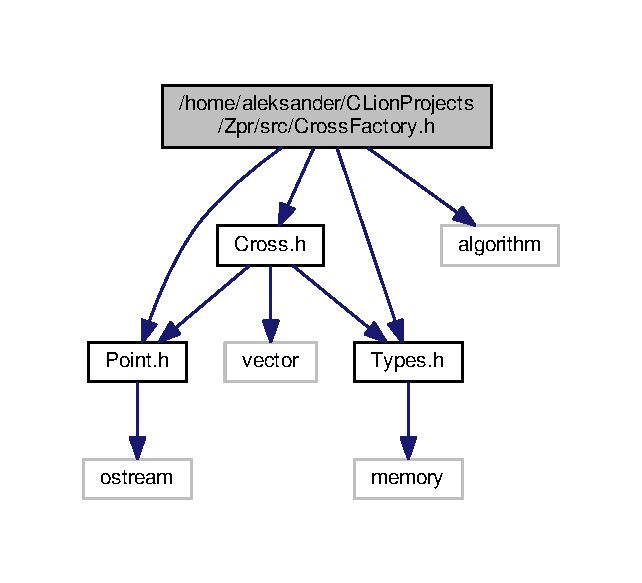
\includegraphics[width=308pt]{CrossFactory_8h__incl}
\end{center}
\end{figure}
This graph shows which files directly or indirectly include this file\-:
\nopagebreak
\begin{figure}[H]
\begin{center}
\leavevmode
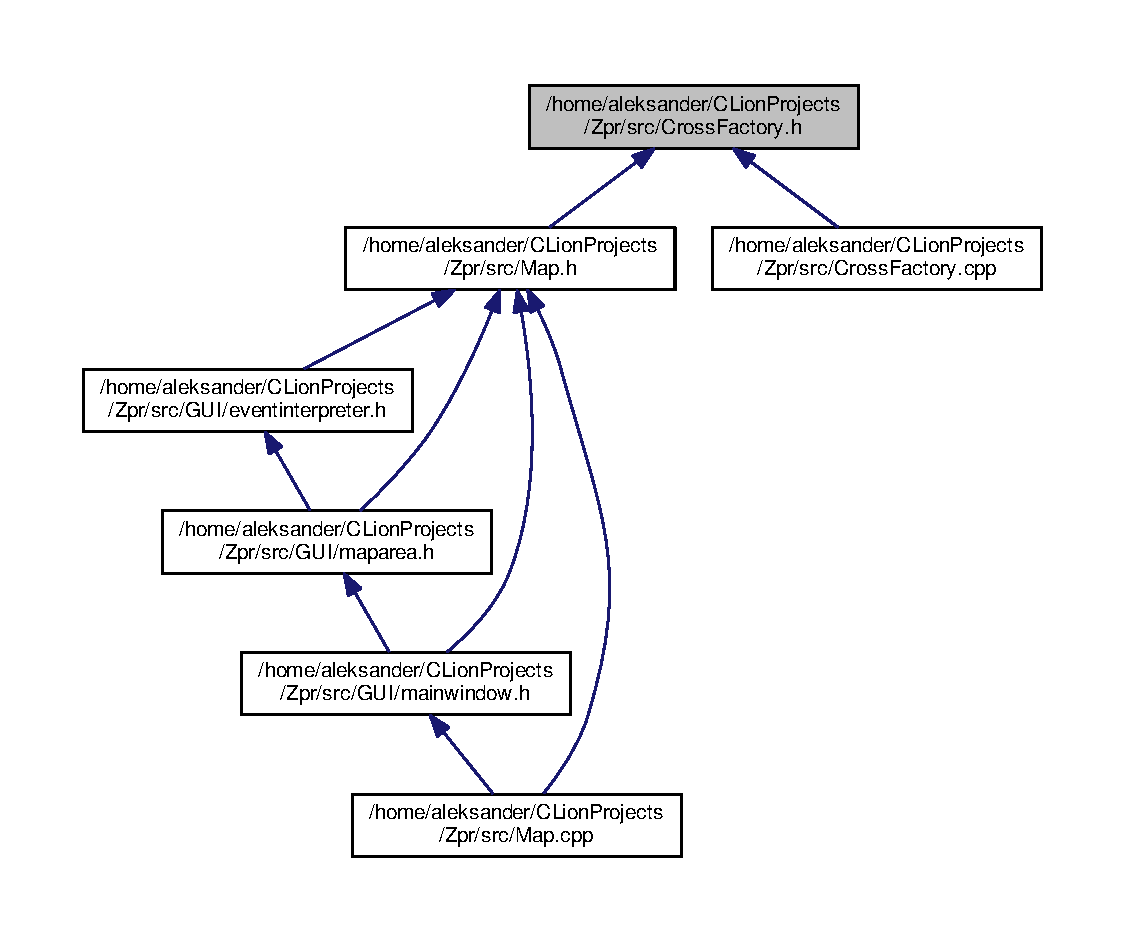
\includegraphics[width=350pt]{CrossFactory_8h__dep__incl}
\end{center}
\end{figure}
\subsection*{Classes}
\begin{DoxyCompactItemize}
\item 
class \hyperlink{classCrossFactory}{Cross\-Factory}
\begin{DoxyCompactList}\small\item\em Factory creating crosses from given roads. \end{DoxyCompactList}\end{DoxyCompactItemize}


\subsection{Detailed Description}
\hyperlink{classCrossFactory}{Cross\-Factory} class methods declaration. Piotr\-Kuc (\href{mailto:piotr.kuc29@gmail.com}{\tt piotr.\-kuc29@gmail.\-com}) \begin{DoxyDate}{Date}
December, 2017 
\end{DoxyDate}

\hypertarget{Map_8cpp}{\section{/home/aleksander/\-C\-Lion\-Projects/\-Zpr/src/\-Map.cpp File Reference}
\label{Map_8cpp}\index{/home/aleksander/\-C\-Lion\-Projects/\-Zpr/src/\-Map.\-cpp@{/home/aleksander/\-C\-Lion\-Projects/\-Zpr/src/\-Map.\-cpp}}
}


\hyperlink{classMap}{Map} class methods implementation.  


{\ttfamily \#include \char`\"{}Map.\-h\char`\"{}}\\*
{\ttfamily \#include $<$G\-U\-I/mainwindow.\-h$>$}\\*
Include dependency graph for Map.\-cpp\-:
\nopagebreak
\begin{figure}[H]
\begin{center}
\leavevmode
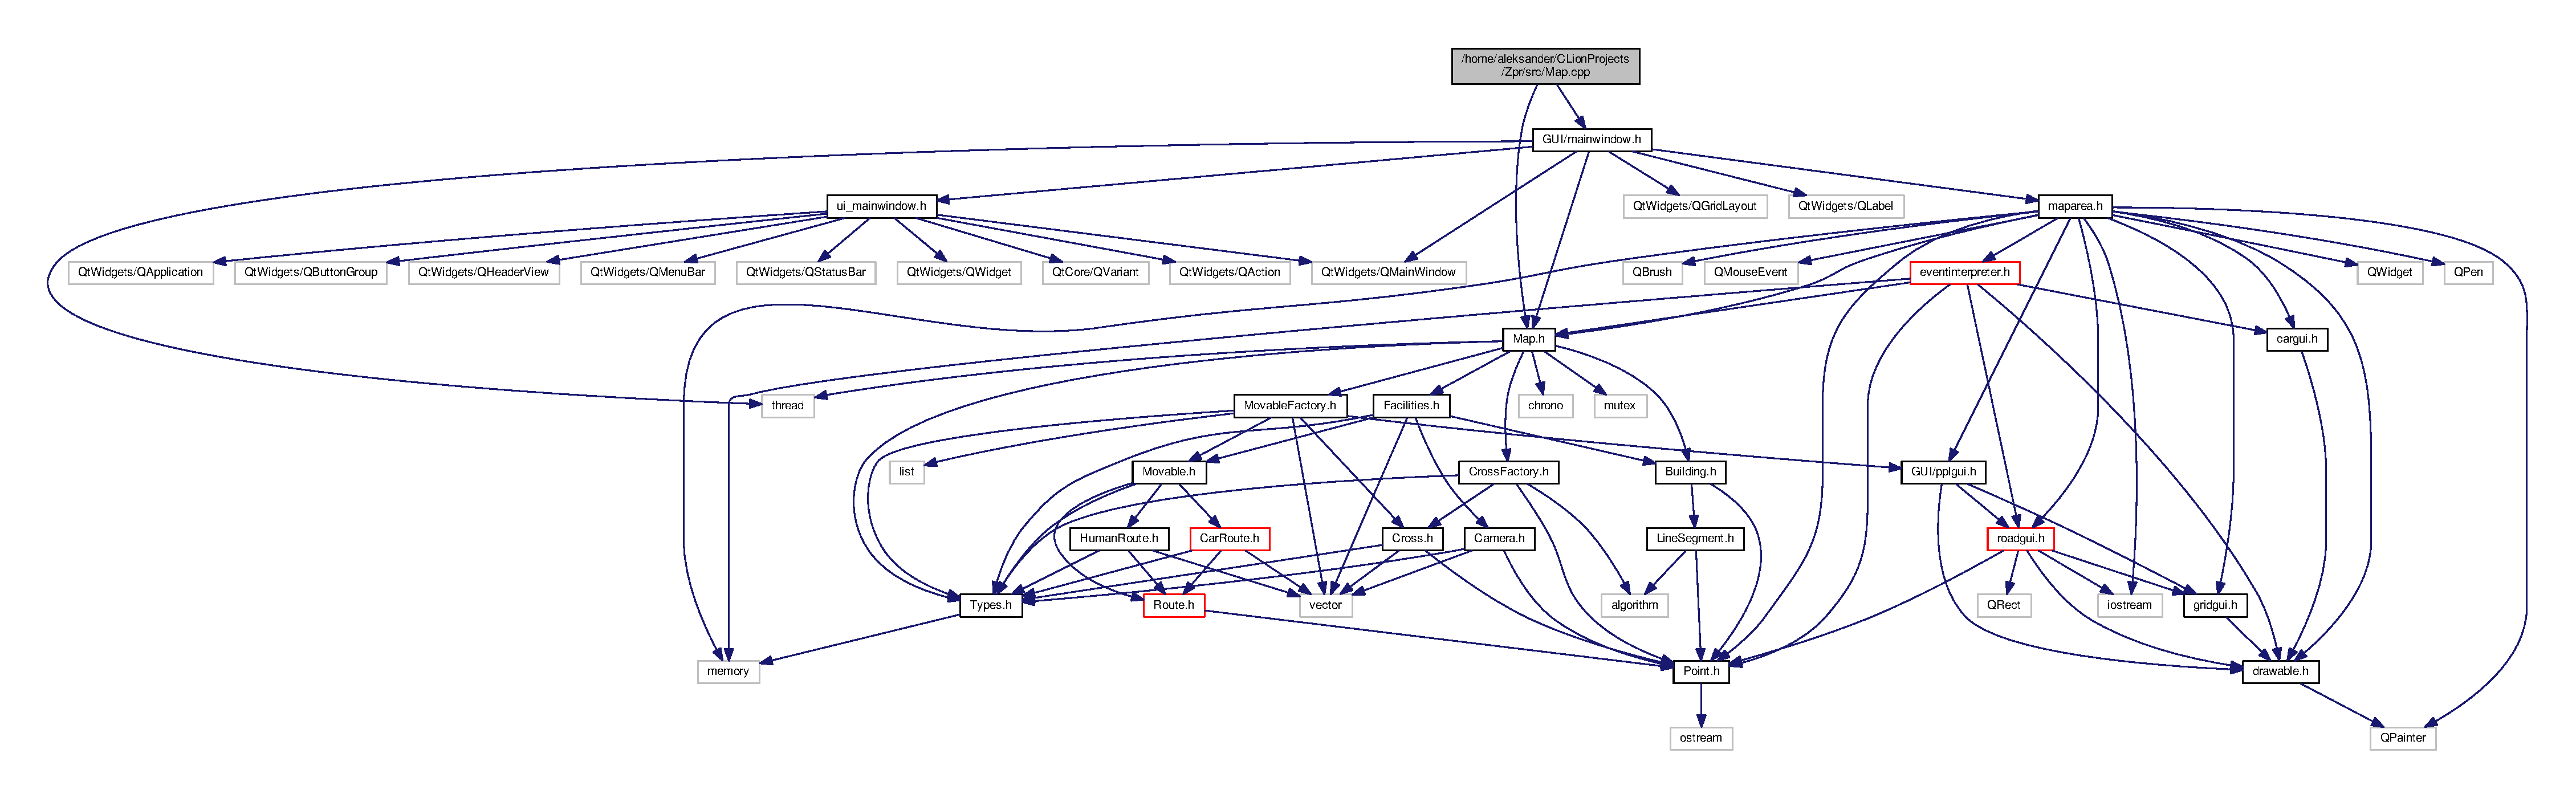
\includegraphics[width=350pt]{Map_8cpp__incl}
\end{center}
\end{figure}


\subsection{Detailed Description}
\hyperlink{classMap}{Map} class methods implementation. Piotr\-Kuc (\href{mailto:piotr.kuc29@gmail.com}{\tt piotr.\-kuc29@gmail.\-com}) \begin{DoxyDate}{Date}
January, 2017 
\end{DoxyDate}

\hypertarget{Map_8h}{\section{/home/aleksander/\-C\-Lion\-Projects/\-Zpr/src/\-Map.h File Reference}
\label{Map_8h}\index{/home/aleksander/\-C\-Lion\-Projects/\-Zpr/src/\-Map.\-h@{/home/aleksander/\-C\-Lion\-Projects/\-Zpr/src/\-Map.\-h}}
}


\hyperlink{classMap}{Map} class declaration.  


{\ttfamily \#include \char`\"{}Movable\-Factory.\-h\char`\"{}}\\*
{\ttfamily \#include \char`\"{}Cross\-Factory.\-h\char`\"{}}\\*
{\ttfamily \#include $<$thread$>$}\\*
{\ttfamily \#include $<$chrono$>$}\\*
{\ttfamily \#include $<$mutex$>$}\\*
{\ttfamily \#include \char`\"{}Types.\-h\char`\"{}}\\*
{\ttfamily \#include \char`\"{}Building.\-h\char`\"{}}\\*
{\ttfamily \#include \char`\"{}Facilities.\-h\char`\"{}}\\*
Include dependency graph for Map.\-h\-:
\nopagebreak
\begin{figure}[H]
\begin{center}
\leavevmode
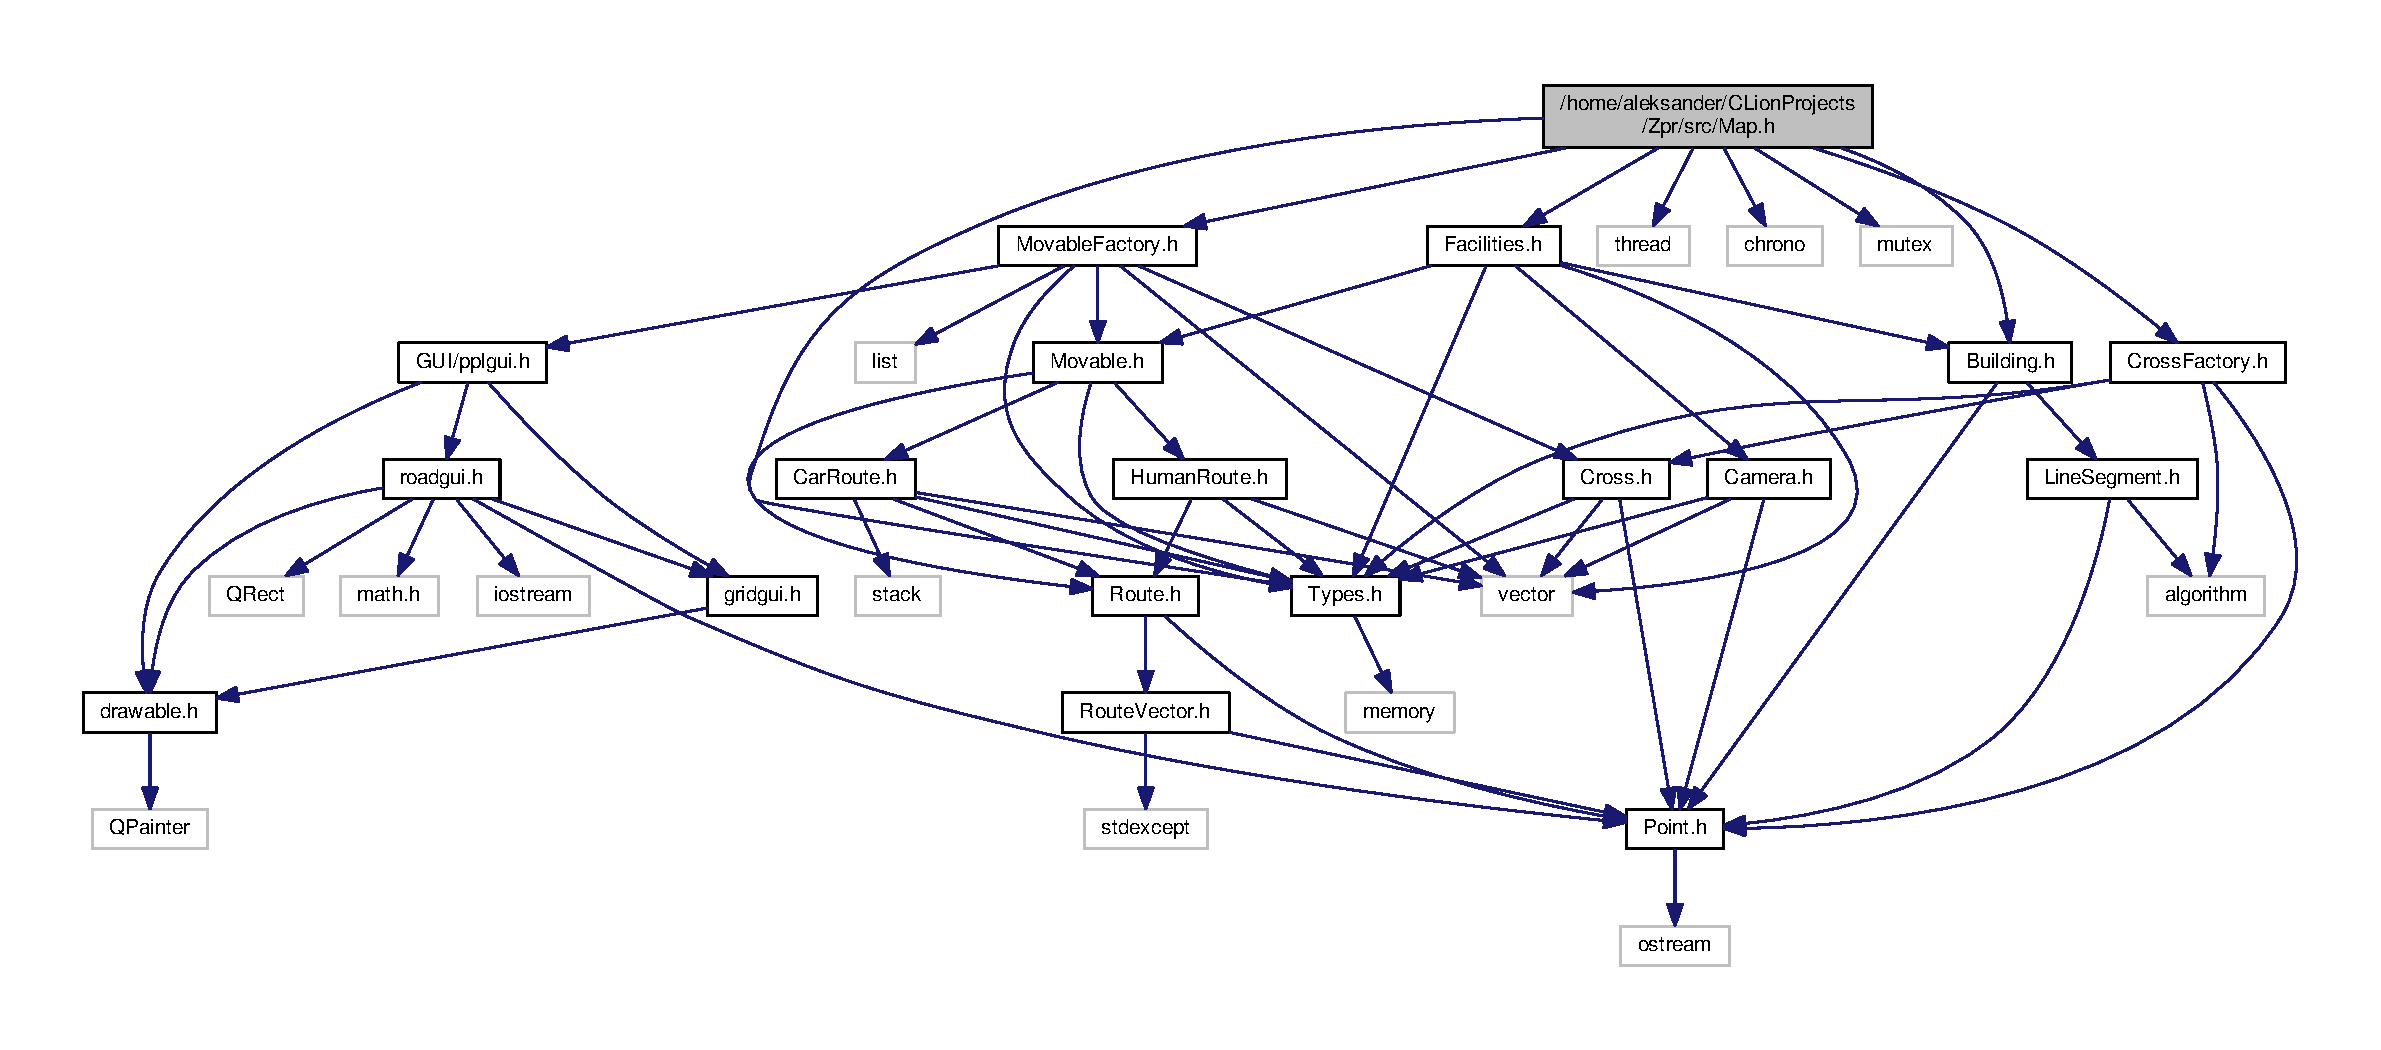
\includegraphics[width=350pt]{Map_8h__incl}
\end{center}
\end{figure}
This graph shows which files directly or indirectly include this file\-:
\nopagebreak
\begin{figure}[H]
\begin{center}
\leavevmode
\includegraphics[width=350pt]{Map_8h__dep__incl}
\end{center}
\end{figure}
\subsection*{Classes}
\begin{DoxyCompactItemize}
\item 
class \hyperlink{classMap}{Map}
\begin{DoxyCompactList}\small\item\em Class allowing to create map and simulate traffics. \end{DoxyCompactList}\end{DoxyCompactItemize}


\subsection{Detailed Description}
\hyperlink{classMap}{Map} class declaration. Piotr\-Kuc (\href{mailto:piotr.kuc29@gmail.com}{\tt piotr.\-kuc29@gmail.\-com}) \begin{DoxyDate}{Date}
January, 2017 
\end{DoxyDate}

\hypertarget{MovableFactory_8cpp}{\section{/home/aleksander/\-C\-Lion\-Projects/\-Zpr/src/\-Movable\-Factory.cpp File Reference}
\label{MovableFactory_8cpp}\index{/home/aleksander/\-C\-Lion\-Projects/\-Zpr/src/\-Movable\-Factory.\-cpp@{/home/aleksander/\-C\-Lion\-Projects/\-Zpr/src/\-Movable\-Factory.\-cpp}}
}


\hyperlink{classMovableFactory}{Movable\-Factory} class methods implementation.  


{\ttfamily \#include $<$algorithm$>$}\\*
{\ttfamily \#include \char`\"{}Movable\-Factory.\-h\char`\"{}}\\*
Include dependency graph for Movable\-Factory.\-cpp\-:
\nopagebreak
\begin{figure}[H]
\begin{center}
\leavevmode
\includegraphics[width=350pt]{MovableFactory_8cpp__incl}
\end{center}
\end{figure}


\subsection{Detailed Description}
\hyperlink{classMovableFactory}{Movable\-Factory} class methods implementation. Piotr\-Kuc (\href{mailto:piotr.kuc29@gmail.com}{\tt piotr.\-kuc29@gmail.\-com}) \begin{DoxyDate}{Date}
January, 2017 
\end{DoxyDate}

\hypertarget{MovableFactory_8h}{\section{/home/aleksander/\-C\-Lion\-Projects/\-Zpr/src/\-Movable\-Factory.h File Reference}
\label{MovableFactory_8h}\index{/home/aleksander/\-C\-Lion\-Projects/\-Zpr/src/\-Movable\-Factory.\-h@{/home/aleksander/\-C\-Lion\-Projects/\-Zpr/src/\-Movable\-Factory.\-h}}
}


\hyperlink{classMovableFactory}{Movable\-Factory} class declaration.  


{\ttfamily \#include \char`\"{}Types.\-h\char`\"{}}\\*
{\ttfamily \#include $<$list$>$}\\*
{\ttfamily \#include $<$vector$>$}\\*
{\ttfamily \#include \char`\"{}Movable.\-h\char`\"{}}\\*
{\ttfamily \#include \char`\"{}Cross.\-h\char`\"{}}\\*
{\ttfamily \#include \char`\"{}G\-U\-I/pplgui.\-h\char`\"{}}\\*
Include dependency graph for Movable\-Factory.\-h\-:
\nopagebreak
\begin{figure}[H]
\begin{center}
\leavevmode
\includegraphics[width=350pt]{MovableFactory_8h__incl}
\end{center}
\end{figure}
This graph shows which files directly or indirectly include this file\-:
\nopagebreak
\begin{figure}[H]
\begin{center}
\leavevmode
\includegraphics[width=350pt]{MovableFactory_8h__dep__incl}
\end{center}
\end{figure}
\subsection*{Classes}
\begin{DoxyCompactItemize}
\item 
class \hyperlink{classMovableFactory}{Movable\-Factory}
\begin{DoxyCompactList}\small\item\em Factory of movables (cars and humans) with algorithms to finding routes. \end{DoxyCompactList}\end{DoxyCompactItemize}


\subsection{Detailed Description}
\hyperlink{classMovableFactory}{Movable\-Factory} class declaration. Piotr\-Kuc (\href{mailto:piotr.kuc29@gmail.com}{\tt piotr.\-kuc29@gmail.\-com}) \begin{DoxyDate}{Date}
January, 2017 
\end{DoxyDate}

%--- End generated contents ---

% Index
\newpage
\phantomsection
\addcontentsline{toc}{chapter}{Index}
\printindex

\end{document}
